\documentclass[semifinal]{cpecmu}

\projectNo{P001-2}
\acadyear{2020}

\titleTH{ระบบจัดตารางสอบปลายภาค}
\titleEN{Final exam scheduling system}

\author{นายกฤษฏิ์ อุปนันท์}{Krit Upanun}{600610717}
\author{นายธนวงศ์ เสนีวงศ์ ณ อยุธยา}{Thanawong Saneewong Na Ayutthaya}{600610738}

\cpeadvisor{chinawat}
\cpecommittee{pruet}
\cpecommittee{sanpawat}%

%% Some possible packages to include:
\usepackage[final]{graphicx} % for including graphics

%% Add bookmarks and hyperlinks in the document.
\PassOptionsToPackage{hyphens}{url}
\usepackage[colorlinks=true,allcolors=Blue4,citecolor=red,linktoc=all]{hyperref}

%% Set up commenting
\iffinal
  \usepackage[disabled]{authcomments}
\else
  \usepackage{authcomments}
\fi
\newcommenter{CI}{0.0,0.5625,0.0}  % green
\newcommenter{TSNA}{0.0,0.0,0.7}
\usepackage{enumitem}

%% Needed just by this example, but maybe not by most reports
\usepackage{afterpage} % for outputting
\usepackage{pdflscape} % for landscape figures and tables. 

\usepackage{forest}
\definecolor{folderbg}{RGB}{124,166,198}
\definecolor{folderborder}{RGB}{110,144,169}
\def\Size{4pt}
\tikzset{
      folder/.pic={
        \filldraw[draw=folderborder,top color=folderbg!50,bottom color=folderbg]
          (-1.05*\Size,0.2\Size+5pt) rectangle ++(.75*\Size,-0.2\Size-5pt);  
        \filldraw[draw=folderborder,top color=folderbg!50,bottom color=folderbg]
          (-1.15*\Size,-\Size) rectangle (1.15*\Size,\Size);
      }
}

\usepackage{multicol}
\usepackage{multirow}
\usepackage{booktabs}
\usepackage{graphicx}

\usepackage{tikz}
\usetikzlibrary{positioning}
\usetikzlibrary{arrows.meta}
\tikzset{>/.tip={Latex[length=2mm]}}
\tikzset{arrow/.style={->}}
\tikzset{double distance=2pt}
\tikzset{flowchart/.style = {node distance=0.75cm and 1cm,
     base/.style = {draw=black,
                    inner sep=1mm, outer sep=0mm,
                    minimum height=1cm,
                    align=flush center},
startstop/.style = {base, rounded corners=5mm, minimum width=1in},
  process/.style = {base, inner xsep=0.5cm},
 decision/.style = {base, diamond, aspect=3},
connector/.style = {draw, circle, minimum size=0pt},
       io/.style = {base, trapezium,
                    trapezium left angle=60, trapezium right angle=-60,
                    trapezium stretches=true},
        io2/.style = {base, trapezium,
                    trapezium left angle=75, trapezium right angle=-75,
                    trapezium stretches=true}
                    }}
%% Some other useful packages. Look these up to find out how to use
%% them.
% \usepackage{natbib}    % for author-year citation styles
% \usepackage{txfonts}
% \usepackage{appendix}  % for appendices on a per-chapter basis
% \usepackage{xtab}      % for tables that go over multiple pages
% \usepackage{subfigure} % for subfigures within a figure
% \usepackage{pstricks,pdftricks} % for access to special PostScript and PDF commands
% \usepackage{nomencl}   % if you have a list of abbreviations

%% if you're having problems with overfull boxes, you may need to increase
%% the tolerance to 9999
% \tolerance=9999

\bibliographystyle{plain}
% \bibliographystyle{IEEEbib}

% \renewcommand{\topfraction}{0.85}
% \renewcommand{\textfraction}{0.1}
% \renewcommand{\floatpagefraction}{0.75}

%% Example for glossary entry
%% Need to use glossary option
%% See glossaries package for complete documentation.
\ifglossary
  \newglossaryentry{lorem ipsum}{
    name=lorem ipsum,
    description={derived from Latin dolorem ipsum, translated as ``pain itself''}
  }
\fi

%% Uncomment this command to preview only specified LaTeX file(s)
%% imported with \include command below.
%% Any other file imported via \include but not specified here will not
%% be previewed.
%% Useful if your report is large, as you might not want to build
%% the entire file when editing a certain part of your report.
% \includeonly{chapters/intro,chapters/background}

\begin{document}
\maketitle
\makesignature

\ifproject
\begin{abstractTH}
เป้าหมายหลักของการจัดการสอบปลายภาคนั้นก็เพื่อที่จะวัดความรู้ความสามารถของนักศึกษา หลังจากจบภาคการศึกษาแล้ว
หากทางมหาวิทยาลัยทำการจัดตารางสอบไม่ดีอาจจะทำให้นักศึกษาบางคนจะต้องสอบสองหรือสามวิชาติดกันในวันเดียว
หรือนักศึกษาบางคนมีวันเว้นว่างระหว่างแต่ละวิชาที่สอบมากเกินไป ซึ่งความไม่สมดุลของตารางสอบนี้อาจจะทำให้นักศึกษาเกิดความเครียดหรือลดทอนกำลังใจในการสอบของนักศึกษาได้
ระบบจัดตารางสอบปลายภาคนี้ เป็นโปรแกรมที่นำวิธีการแก้ปัญหาการระบายสีกราฟมาประยุกต์ใช้ในการจัดตารางสอบปลายภาคจากข้อมูลการลงทะเบียนของนักศึกษาหลังจากการลงทะเบียนเสร็จสิ้นแล้ว เพื่อให้ได้ตารางสอบที่มีการกระจายตัวของวิชาที่สอบอย่างมีความสมดุล
ลดจำนวนนักศึกษาที่ต้องสอบสองวิชาติดกันในหนึ่งวันให้น้อยที่สุด โดยตารางสอบของนักศึกษาคนใด ๆ ต้องไม่มีวิชาที่สอบตรงกัน ช่วยลดช่วงวันเว้นว่างของนักศึกษาในการสอบ 
และยังช่วยให้นักศึกษาสามารถเลือกลงทะเบียนวิชาเรียนที่สนใจได้อย่างอิสระโดยไม่ต้องกังวลว่าตารางสอบของวิชาที่ต้องการลงทะเบียนจะทับซ้อนกัน
\CIreply{เขียนผลลัพธ์จากการ implement เช่น เวลาที่ใช้ และผลการสำรวจความพึงพอใจเพิ่มโดยสังเขป}
\end{abstractTH}

\begin{abstract}
The main goal of scheduling final exams is to have every student take an exam for every course they registered for that semester to assess their knowledge and learning ability.
Without careful planning, the final exam schedule for a particular student might require that the student take two or three final exams consecutively or create a gap too long between two exams make an imbalance that affects the stress level of the student.
"Final exam scheduling system" is a program that applies a graph-coloring algorithm to solve the final exam scheduling problem. The system uses data from student registration to create a balanced final exam schedule. The goal of this system is to reduce the number of students who need to take exams consecutively,
to reduce the gap between each exam, and—importantly—to enable students to enroll in any course they want to without worrying about the final exam schedule. The final exam schedule for every student produced from this system must not have overlapping courses.
\CIreply{CI TODO: check after rewriting Thai abstract}
\end{abstract}

\iffalse
\begin{dedication}
This document is dedicated to all Chiang Mai University students.

Dedication page is optional.
\end{dedication}
\fi % \iffalse

\begin{acknowledgments}
โครงงานนี้ได้รับความกรุณาจาก อ.ดร.ชินวัตร อิศราดิสัยกุล อาจารย์ที่ปรึกษา ที่ได้สละเวลาให้ความช่วยเหลือทั้งให้คำแนะนำ ให้ความรู้และแนวคิดต่าง ๆ รวมถึง อ.ดร.พฤษภ์ บุญมา และ รศ.ดร.สรรพวรรธน์ กันตะบุตร ที่ให้คำปรึกษาจนทำให้โครงงานเล่มนี้เสร็จสมบูรณ์ไปได้
    
ขอขอบคุณงานบริการการศึกษาและพัฒนาคุณภาพนักศึกษา คณะต่าง ๆ ใน มหาวิทยาลัยเชียงใหม่ ที่ได้ให้ความร่วมมือเป็นอย่างดีในการให้ข้อมูลอันเป็นประโยชน์ต่อการพัฒนาโครงงานนี้

ขอขอบคุณเพื่อน ๆ ที่ช่วยให้ข้อมูลอันเป็นประโยชน์ต่อการทำโครงงาน และช่วยให้กำลังใจ รวมถึงคำแนะนำที่ดีตลอดการทำโครงงานที่ผ่านมา

ขอขอบคุณนักศึกษาทุกคนที่ช่วยให้ความร่วมมือในการตอบแบบสอบถาม ช่วยแสดงความคิดเห็นพร้อมทั้งข้อเสนอแนะเกี่ยวกับช่วงเวลาที่ต้องการจะสอบ ซึ่งเป็นข้อมูลที่สำคัญที่ใช่ในการออกแบบและพัฒนาโครงงานให้สำเร็จลุล่วง

ขอขอบคุณร้านอาหารต่าง ๆ ที่ให้สถานที่ในการประชุมแต่ละครั้ง พร้อมทั้งยังทำให้อิ่มท้องทำให้สามารถใช้ความคิดได้ดีมากยิ่งขึ้น

นอกจากนี้ผู้จัดทำขอขอบพระคุณ บิดา มารดา และครอบครัวที่ได้คอยให้คำแนะนำและ ให้กำลังใจ ตลอดมา รวมทั้งขอขอบพระคุณอีกหลาย ๆ ท่านที่ไม่ได้เอ่ยนามมา ณ ที่นี้ ที่ได้ให้ความช่วยเหลือจนทำให้โครงงานนี้สำเร็จลงได้ 


\acksign{2021}{4}{2}
\end{acknowledgments}%
\fi % \ifproject

\contentspage

\ifproject
\figurelistpage

\tablelistpage
\fi % \ifproject

% \abbrlist % this page is optional

% \symlist % this page is optional

% \preface % this section is optional


\pagestyle{empty}\cleardoublepage
\normalspacing \setcounter{page}{1} \pagenumbering{arabic} \pagestyle{cpecmu}

\chapter{\ifcpe บทนำ\else Introduction\fi}

\section{\ifcpe ที่มาของโครงงาน\else Project rationale\fi}
\label{sec:project_rationale}


การสอบปลายภาคหรือการทดสอบความรู้ในช่วงท้ายของการเรียนเป็นส่วนหนึ่งในการวัดระดับความรู้ที่นักศึกษาได้เรียนรู้ไปในวิชานั้น ๆ 
ซึ่งสามารถบ่งบอกถึงความเข้าใจ เอาใจใส่ของนักศึกษาคนนั้น ๆ ซึ่งปัจจัยที่มีผลต่อการสอบนั้นมีอยู่หลายปัจจัย 
ตัวอย่างเช่น ความตั้งใจ ความพยายาม ความเอาใจใส่กับรายวิชาของนักศึกษา แต่ก็ยังมีปัจจัยอีกหนึ่งปัจจัยที่มีผลต่อการสอบปลายภาคด้วย 
คือตารางสอบปลายภาคของนักศึกษา โดยตารางสอบนั้นอาจจะส่งผลกระทบต่อนักศึกษาหากทางมหาวิทยาลัยมีการจัดตารางสอบไม่ดีพอ 
ซึ่งในที่นี้จะกล่าวถึงการจัดตารางสอบของมหาวิทยาลัยเชียงใหม่ ซึ่งในแต่ละภาคการศึกษานั้นมีนักศึกษาที่เรียนมากกว่า 30,000 คน 
มีวิชาที่เปิดให้ลงทะเบียนมากกว่า 3000 วิชา มีคู่วิชาที่มีนักศึกษาลงทะเบียนพร้อมกันอย่างน้อย 1 คน มากกว่า 30000 คู่วิชา 
โดยตารางสอบนั้นจะเป็นตารางที่ถูกจัดไว้ก่อนการลงทะเบียนเรียนของนักศึกษา และการลงทะเบียนเรียนนักศึกษาจะต้องเลือกลงทะเบียนไม่ให้มีวิชาที่สอบตรงกัน 
ไม่อย่างนั้นหากนักศึกษาไม่ได้พิจารณาเวลาสอบให้ดีก่อนการลงทะเบียน นักศึกษาจะต้องถอนวิชาใดวิชาหนึ่งที่เวลาสอบตรงกันออก หรือจะได้รับผลการประเมินขั้น “F” ในวิชาที่ไม่สามารถเข้าสอบปลายภาคได้


ทางมหาวิทยาลัยเชียงใหม่คาดหวังว่านักศึกษาจะเลือกลงทะเบียนเรียนวิชาต่าง ๆ โดยเลือกลงวิชาที่เวลาเรียนไม่ตรงกัน 
ดังนั้นทางมหาวิทยาลัยจึงจัดตารางสอบของนักศึกษาโดยจัดตารางให้กับวิชาที่มีตอนเดียวก่อน โดยจะอ้างอิงตามช่วงเวลาที่เรียน 
วิชาที่เรียนในวันและเวลาเดียวกันจะถูกจัดให้สอบในช่วงเวลาเดียวกัน (เรียกการจัดสอบแบบนี้ว่า Regular Exam ดังแสดงในรูปที่ \ref{fig:regular_exam}) 
ส่วนวิชาที่มีหลายตอนจะถูกจัดให้สอบในช่วงเวลาที่ไม่ตรงกับเวลาสอบของวิชาที่มีตอนเดียว  (เรียกการจัดสอบแบบนี้ว่า Special Exam ดังแสดงในรูปที่ \ref{fig:special_exam}) 
เพื่อให้นักศึกษาที่ลงทะเบียนวิชาเดียวกันในเวลาที่ต่างกัน  (ลงทะเบียนวิชาเดียวกันแต่คนละตอน) สามารถสอบในเวลาเดียวกันได้ เพื่อเป็นการป้องกันข้อสอบรั่วไหล 
ซึ่งการจัดตารางสอบในลักษณะดังกล่าวนั้นทําให้นักศึกษาไม่สามารถลงทะเบียนวิชาที่สนใจได้อย่างอิสระเนื่องจากตารางสอบตรงกันหรือเวลาสอบของสองวิชาที่ต้องการลงทะเบียนนั้นติดกันมากเกินไป นอกจากนี้ การจัดตารางสอบด้วยวิธีนี้ ทำให้บางวิชานั้นสามารถกําหนดวันสอบให้อยู่ในช่วงท้าย ๆ ของฤดูกาลสอบได้ 
ทําให้นักศึกษาบางคนมีวันเว้นว่างระหว่างการสอบหลายวันเพราะจําเป็นต้องอยู่รอทำการสอบในวิชาท้าย ๆ ซึ่งปัญหาดังที่กล่าวมานี้ก็อาจเกิดขึ้นกับมหาวิทยาลัยอื่น ๆ ที่มีวิธีการจัดการกับตารางสอบในรูปแบบที่คล้าย ๆ กันนี้เช่นกัน


จากในงานวิจัยของ Ender {\"O}zcan (2005) \cite{fes} ได้เคยมีการสร้างโปรแกรมสำหรับจัดตารางสอบมาก่อนโดยมีการจัดตารางสอบแบ่งเป็นตารางสอบของวิชาภายในคณะและวิชาภายในภาควิชา 
ซึ่งไม่สามารถใช้ได้กับวิชาเรียนของทางมหาวิทยาลัยเชียงใหม่ เนื่องจากมีวิชาด้านการศึกษาทั่วไปที่มีนักศึกษาจากต่างคณะสามารถลงทะเบียนเรียนร่วมกันได้


จากปัญหาข้างต้น ทีมผู้พัฒนาคาดว่าการพัฒนาระบบจัดตารางสอบโดยใช้ข้อมูลลงทะเบียนของนักศึกษา หลังจากการลงทะเบียนเสร็จสิ้นแล้ว 
จะช่วยให้นักศึกษามีอิสระในการเลือกลงวิชาเรียนมากขึ้นช่วยลดจำนวนนักศึกษาที่ต้องสอบสองวิชาติดกันในหนึ่งวันให้น้อยลง และลดวันเว้นว่างระหว่างช่วงเวลาสอบ
ซึ่งจะช่วยลดความเครียดส่วนหนึ่งในช่วงสอบของนักศึกษาได้
\begin{figure}
    \begin{center}
      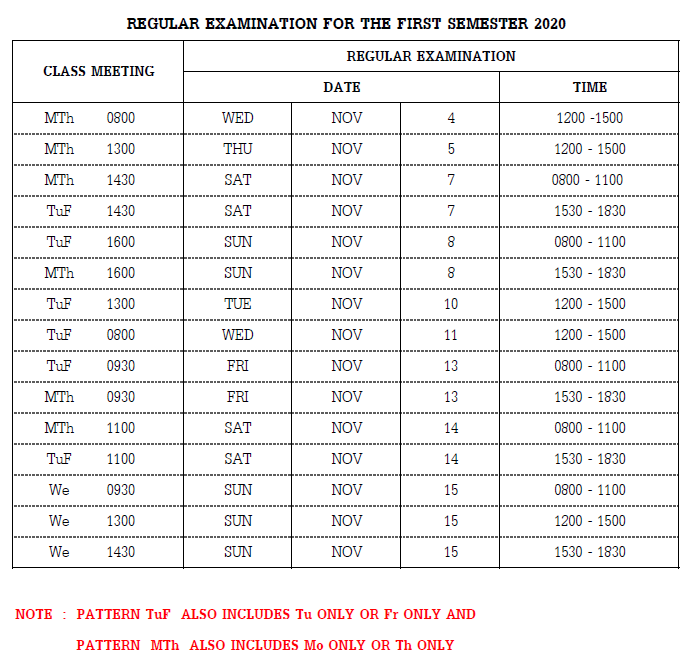
\includegraphics[width=\linewidth]{images/regular_exam.png}
    \end{center}
    \caption[ตัวอย่างตารางสอบ regular exam เทอม 1/2563]{ตัวอย่างตารางสอบ regular exam เทอม 1/2563}
    \label{fig:regular_exam}     
\end{figure}
\begin{figure}
    \begin{center}
      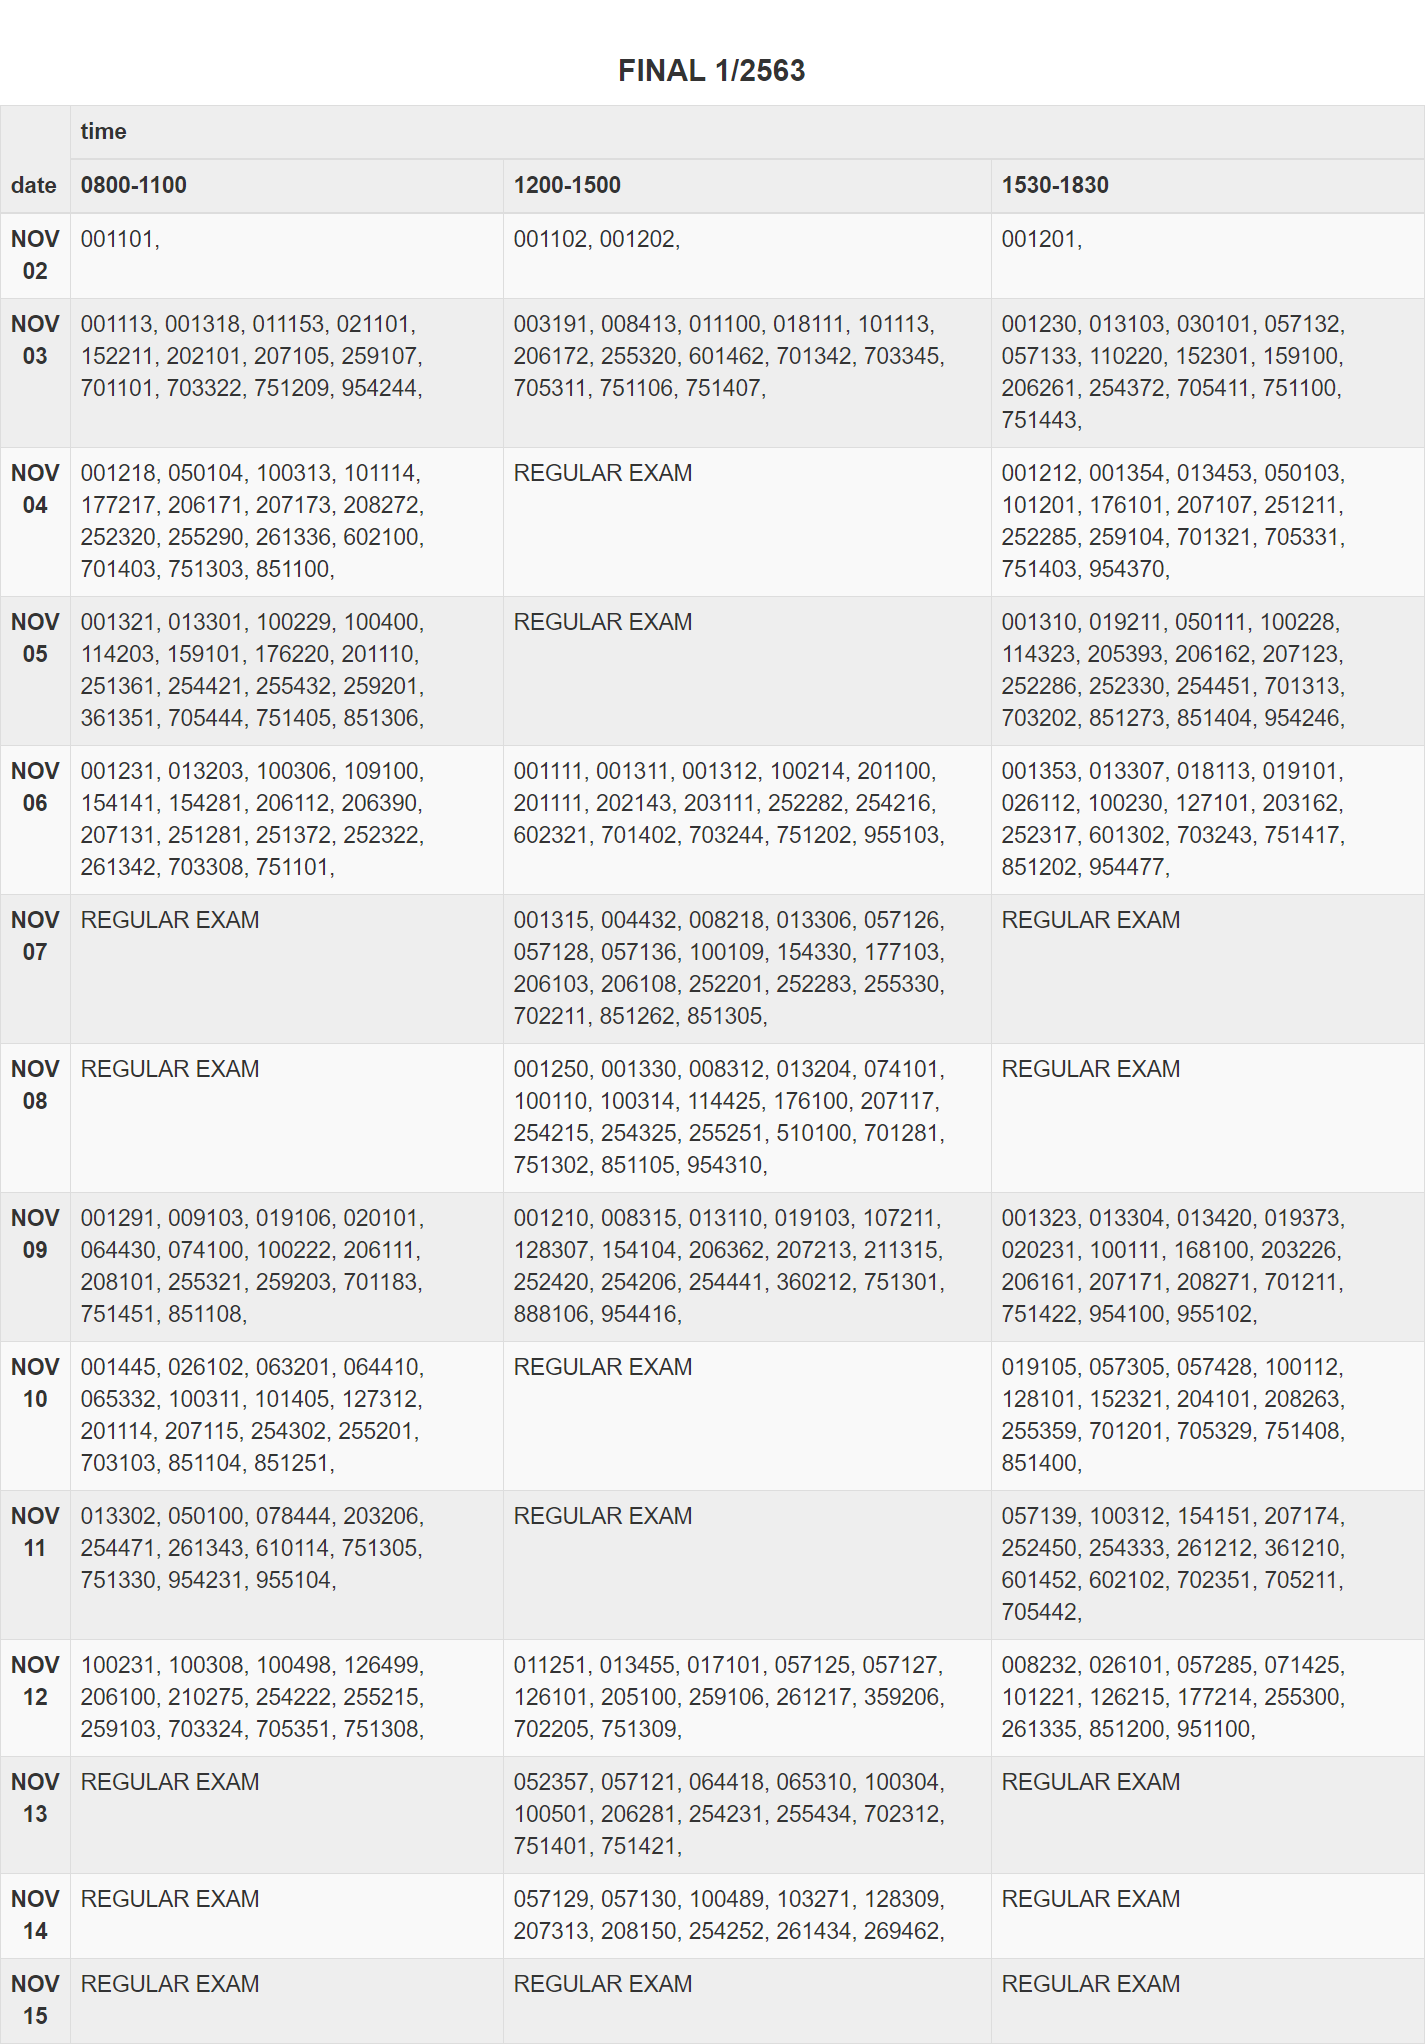
\includegraphics[width=\linewidth]{images/special_exam.png}
    \end{center}
    \caption[ตัวอย่างตารางสอบ special exam เทอม 1/2563]{ตัวอย่างตารางสอบ special exam เทอม 1/2563}
    \label{fig:special_exam}     
\end{figure}
\newpage
\section{\ifcpe วัตถุประสงค์ของโครงงาน\else Objectives\fi}
\label{sec:Objectives}
\begin{enumerate}
    \item เพื่อพัฒนาโปรแกรมสำหรับจัดตารางสอบปลายภาคในมหาวิทยาลัย จากข้อมูลการลงทะเบียนของนักศึกษา โดยตารางสอบที่ได้มีคุณสมบัติ ดังนี้
    \begin{itemize}
        \item ต้องไม่มีนักศึกษาคนใด ๆ ถูกกำหนดให้สอบสองวิชาในเวลาเดียวกัน
        \item จำนวนนักศึกษาที่มีสอบหลายวิชาติดกันในวันเดียว ลดลงจากตารางสอบดั้งเดิม
        \item จำนวนนักศึกษาที่มีช่วงวันที่เว้นจากการสอบวิชาก่อนหน้ามากกว่า 3 วัน ลดลงจากตารางสอบดั้งเดิม
        \item ในแต่ละช่วงเวลาที่จัดสอบ จำนวนนักศึกษาที่สอบจะต้องไม่เกินจำนวนที่นั่งสอบที่ทางมหาวิทยาลัยสามารถจัดให้ได้
    \end{itemize}
    \item เพื่อแก้ไขปัญหานักศึกษาไม่สามารถลงทะเบียนในรายวิชาที่ต้องการได้อย่างอิสระ เนื่องจากตารางสอบของรายวิชาที่ต้องการลงทะเบียนถูกจัดไว้ล่วงหน้าให้สอบในช่วงเวลาเดียวกัน
\end{enumerate}

\section{\ifcpe ขอบเขตของโครงงาน\else Project scope\fi}
เป้าหมายของโครงงานนี้ ต้องการพัฒนาโปรแกรมสำหรับจัดตารางสอบปลายภาคในระดับมหาวิทยาลัย
โดยโครงงานนี้จะพิจารณาความต้องการและข้อจำกัดต่าง ๆ ที่ใช้ในการจัดตารางสอบของมหาวิทยาลัยเชียงใหม่
และจะพิจารณาเฉพาะข้อจำกัดทางด้านเวลาเท่านั้น โดยมีขอบเขตของโครงงานดังนี้ 
\subsection{\ifcpe ขอบเขตด้านฮาร์ดแวร์\else Hardware scope\fi}
\begin{enumerate}
    \item ระบบที่จะพัฒนานั้นจะสามารถทำงานได้บนคอมพิวเตอร์ที่ใช้ระบบปฏิบัติการ Windows 7 / Windows 10 หรือระบบปฏิบัติการ Linux เท่านั้น
\end{enumerate}
\subsection{\ifcpe ขอบเขตด้านซอฟต์แวร์\else Software scope\fi}
\begin{enumerate}
    \item ระบบที่จะพัฒนานั้นจะสามารถทำงานได้หากติดตั้ง Python 3.6 ขึ้นไป เท่านั้น \TSNAreply{ไม่แน่ใจ ใส่ไว้ก่อน}
\end{enumerate}
\subsection{ข้อจำกัดที่นำมาพิจารณาในการจัดตารางสอบ}
\begin{enumerate}
    \item ระยะเวลาที่ใช้ในการจัดสอบปลายภาค คือ 2 สัปดาห์
    \item จำนวนช่วงเวลาที่จัดสอบในแต่ละวัน คือ 3 ช่วงเวลา ได้แก่ 8:00--11:00, 12:00--15:00 
    และ 15:30--18:30
    \item จำนวนที่นั่งสอบที่มหาวิทยาลัยสามารถจัดให้ได้ในตึกอาคารเรียนรวม
    \item จำนวนที่นั่งสอบในแต่ละห้องสอบของแต่ละคณะ
    \item รายชื่อวิชาเรียนที่มีการจัดสอบปลายภาค
    \item ข้อมูลจากการลงทะเบียนล่วงหน้าและลงทะเบียนรอบปกติ
    \item คู่วิชาเรียนที่มีนักศึกษาลงทะเบียนร่วมกันทั้งสองวิชา โดยคู้่วิชาที่มีจำนวนนักศึกษาลงทะเบียนมาก จะมีลำดับความสำคัญสูงกว่า
\end{enumerate}

\subsection{ข้อจำกัดที่ไม่นำมาพิจารณาในการจัดตารางสอบ}
\begin{enumerate}
    \item การจัดอาจารย์ผู้คุมสอบให้กับแต่ละรายวิชา
    \item เวลาที่จัดการเรียนการสอนของแต่ละรายวิชา
    \item การจัดตารางสอบแยกตามรายวิชาของแต่ละคณะ หรือแต่ละภาควิชา
    \item ข้อมูลจากการลงทะเบียนเพิ่มเติมหลังกำหนด
\end{enumerate}

\section{\ifcpe ประโยชน์ที่ได้รับ\else Expected outcomes\fi}
\begin{enumerate}
    \item นักศึกษาสามารถเลือกลงทะเบียนวิชาที่ต้องการได้อย่างอิสระ โดยไม่ต้องกังวลเรื่องตารางสอบจะถูกจัดให้สอบในช่วงเวลาเดียวกัน
    \item ช่วยให้ตารางสอบของนักศึกษาคนใด ๆ มีจำนวนรายวิชาที่ต้องสอบในแต่ละวันน้อยลง
    \item ช่วยลดวันเว้นว่างระหว่างช่วงเวลาสอบของนักศึกษาให้น้อยลง 
\end{enumerate}

\section{\ifcpe เทคโนโลยีและเครื่องมือที่ใช้\else Technology and tools\fi}

% \subsection{\ifcpe เทคโนโลยีด้านฮาร์ดแวร์\else Hardware technology\fi}
% \begin{enumerate}

% \end{enumerate}
\subsection{\ifcpe เทคโนโลยีด้านซอฟต์แวร์\else Software technology\fi}
\begin{enumerate}
\iffalse   
\item Google OR-Tools
\item Gurobi Optimizer
\fi
    \item Visual Studio Code
    \item Python
    \item Node.js
    \item Vue.js
\end{enumerate}

\section{\ifcpe แผนการดำเนินงาน\else Project plan\fi}

\begin{plan}{7}{2020}{3}{2021}
    \planitem{7}{2020}{10}{2020}{Literature Review}
    \planitem{9}{2020}{10}{2020}{เก็บข้อมูลความคิดเห็นนักศึกษา}
    \planitem{10}{2020}{10}{2020}{เขียนรายงาน}
    \planitem{11}{2020}{12}{2020}{เก็บข้อมูลรายวิชาที่ไม่จัดการสอบ}
    \planitem{11}{2020}{12}{2020}{ออกแบบอัลกอริทึม เวอร์ชัน 1}
    \planitem{12}{2020}{12}{2020}{ทดสอบและประเมินผลอัลกอริทึม}
    \planitem{12}{2020}{1}{2021}{เก็บข้อมูลความจุที่นั่งสอบของแต่ละคณะและอาคารส่วนกลาง}
    \planitem{12}{2020}{1}{2021}{ออกแบบอัลกอริทึม เวอร์ชัน 2}
    \planitem{1}{2021}{2}{2021}{ทดสอบและประเมินผลอัลกอริทึม}
    \planitem{2}{2021}{3}{2021}{เก็บข้อมูลความพึงพอใจและความคิดเห็นของนักศึกษา}
    \planitem{2}{2021}{3}{2021}{สรุปผลการพัฒนาโปรแกรม}
    \planitem{3}{2021}{3}{2021}{เขียนรายงานผลการพัฒนาโปรแกรม}
\end{plan}

\section{\ifcpe บทบาทและความรับผิดชอบ\else Roles and responsibilities\fi}
\begin{itemize}
\item นายกฤษฏิ์ อุปนันท์: รับผิดชอบหน้าที่ในการเก็บรวบรวมและสรุปผลความคิดเห็นและความต้องการของนักศึกษา
จากแบบสำรวจเพื่อนำมาใช้ในการจัดลำดับความสำคัญของตัวชี้วัดที่ใช้ในการประเมินระบบ
\item นายธนวงศ์ เสนีวงศ์ ณ อยุธยา: รับผิดชอบหน้าที่ในการศึกษาทฤษฎีที่เกี่ยวข้องและอัลกอริทึมที่จำเป็นต้องใช้ในการพัฒาระบบ
\end{itemize}

ในส่วนของการออกแบบอัลกอริทึมและเขียนโปรแกรมเพื่อพัฒนาระบบ ทั้งสองคนจะช่วยกันออกแบบและพัฒนาโดยแบ่งงานกันอย่างเท่าเทียม

\section{\ifcpe%
ผลกระทบด้านสังคม สุขภาพ ความปลอดภัย กฎหมาย และวัฒนธรรม
\else%
Impacts of this project on society, health, safety, legal, and cultural issues
\fi}

ผลกระทบทางด้านสังคม: ระบบที่เป็นผลลัพธ์ของโครงงานนี้จะสามารถใช้เป็นทางเลือกในการจัดการตารางสอบในระดับมหาวิทยาลัยได้
ซึ่งตารางสอบที่ได้จากโปรแกรมนี้จะช่วยให้นักศึกษาสามารถเลือกเรียนวิชาที่ตนเองต้องการได้อย่างอิสระ โดยไม่มีข้อจำกัดด้านตารางสอบ
เหมือนอย่างระบบเดิมที่ใช้อยู่ในปัจจุบัน อีกทั้งหากมีการนำไปประยุกต์ใช้กับการจัดตารางสอบที่อื่นที่คณาจารย์ยังคงต้องจัดตารางสอบด้วยตัวเองอยู่
จะเป็นการช่วยลดภาระการจัดตารางสอบของคณาจารย์ได้
\chapter{\ifcpe ทฤษฎีที่เกี่ยวข้อง\else Background Knowledge and Theory\fi}

การทำโครงงานนี้เริ่มต้นจากการที่เราเล็งเห็นปัญหาของตารางสอบปลายภาคของมหาวิทยาลัยเชียงใหม่ 
ซึ่งตารางสอบของนักศึกษาบางคนอาจจะมีตารางเวลาที่ติดกันมากเกินไป ซึ่งผู้จัดทำเห็นว่าปัญหาการจัดตารางสอบปลายภาค
สามารถแปลงเป็นปัญหาที่มีวิธีในการแก้ไขอยู่แล้วได้ ในบทนี้จะกล่าวถึงผลการศึกษาค้นคว้าทฤษฎีที่เกี่ยวข้อง งานวิจัย หรือโครงงาน ที่เคยมีผู้นำเสนอไว้แล้ว
เพื่อช่วยอธิบายถึงสิ่งต่าง ๆ ที่เกี่ยวข้องกับโครงงานนี้เพื่อให้ผู้อ่านเข้าใจเนื้อหาในบทถัด ๆ ไปได้ง่ายยิ่งขึ้น โดยในบทนี้จะมีเนื้อหาต่าง ๆ ได้แก่ Literature review 
ซึ่งจะกล่าวถึงงานวิจัยต่าง ๆ ที่ได้ศึกษามา และส่วนของอัลกอลิทึมที่เกี่ยวข้อง ซึ่งจะกล่าวถึงรูปแบบและวิธีการทำงานของอัลกอลิทึมต่าง ๆ 
\section{Literature review}
การกำหนดเวลาสอบปลายภาคเพื่อหลีกเลี่ยงปัญหานักศึกษาคนใด ๆ มีเวลาสอบในช่วงเวลาเดียวกันสามารถแปลงปัญหานี้ให้เป็นปัญหา graph coloring~\cite{mcs} ได้ 
โดยที่จุดแต่ละจุดในกราฟเป็นรายวิชาที่เปิดสอนในภาคการศึกษานั้น 
และเส้นที่เชื่อมแต่ละจุดสองจุดในกราฟแสดงถึงการมีนักศึกษาที่ลงทะเบียนเรียนทั้งสองรายวิชา โดยจุดสองจุดใด ๆ ในกราฟที่มีเส้นเชื่อมกันจะถูกกำหนดสีให้ต่างกัน
ซึ่งแสดงถึงวันและเวลาที่จัดสอบปลายภาคในวิชานั้น ๆ โดยจุดที่มีคนละสีก็จะถูกจัดให้สอบคนละช่วงเวลากัน

การแปลงปัญหาการจัดตารางสอบปลายภาคให้เป็นปัญหา graph coloring จะสามารถแก้ปัญหาการจัดตารางสอบแบบพื้นฐานได้เท่านั้น โดยไม่คำนึงถึงข้อจำกัดอย่างอื่น 
ตัวอย่างเช่น ไม่พิจารณาความจุที่นั่งสำหรับการสอบแต่ละช่วงเวลาของนักศึกษา จำนวนอาจารย์ที่คุมสอบแต่ละช่วงเวลา และการกระจายวิชาสอบสำหรับนักศึกษาแต่ละคน เป็นต้น
ถึงแม้จะไม่กำหนดข้อจำกัดใด ๆ ปัญหา graph coloring ก็เป็นปัญหา NP-complete ด้วยตัวมันเองอยู่แล้ว~\cite{alg-design} 
ซึ่งหมายความว่ายังไม่สามารถหาอัลกอริทึมที่ใช้เวลา polynomial-time ในการแก้ไขปัญหาให้ได้ผลลัพธ์ที่เหมาะสมที่สุด 
ทำให้ต้องใช้วิธีอื่นที่ให้ผลลัพธ์ที่ดีในระดับที่ยอมรับได้ แต่สามารถยืนยันได้ว่าจะได้วิธีการที่สามารถแก้ไขปัญหาได้อย่างแน่นอน 
ซึ่งวิธีการนั้นคือ metaheuristic ซึ่งสามารถหาวิธีการแก้ปัญหาที่ดีได้ในระยะเวลาที่เหมาะสม~\cite{meta-for-vertexcolor}
และสามารถกำหนดข้อจำกัดหรือเงื่อนไขอื่นเพิ่มเติมได้ ทำให้สามารถกำหนดขอบเขตของผลลัพธ์ได้ แต่อาจจะไม่ได้วิธีแก้ปัญหาที่ดีที่สุด

อีกวิธีการที่สามารถใช้แก้ไขปัญหาการจัดตารางสอบได้ก็คือการใช้ memetic algorithms (MA) ซึ่งเป็นวิธีการที่นำ local search มาประยุกต์ใช้กับ genetic algorithm 
เพื่อช่วยลดระยะเวลาให้คำตอบของปัญหานั้น converge ช้าลง \cite{pablo-memetic-algo} ซึ่ง Ender {\"O}zcan เคยได้นำวิธีการนี้มาประยุกต์ใช้ในการแก้ปัญหาการจัดตารางสอบ 
โดยได้สร้าง Framework สำหรับออกแบบตัวดำเนินการที่ใช้ในการ crossover และ mutation ของ genetic algorithm ด้วย~\cite{fes}
โดยในการทดลองนี้ได้มีการคำนึงถึงนักศึกษา โดยกำหนดข้อจำกัดของตารางสอบที่ได้ให้ไม่มีนักศึกษาที่ต้องสอบติดกันสองวิชาในแต่ละวัน แต่การจัดตารางสอบในแบบของ Ender 
นั้นเป็นการจัดตารางสอบของมหาวิทยาลัย Yeditepe โดยแบ่งตารางสอบเป็นของภาควิชาต่าง ๆ และแบ่งย่อยแยกตามสาขาวิชาอีกที วิธีการนี้ไม่สามารถนำมาใช้กับการจัดตารางสอบของมหาวิทยาลัยเชียงใหม่ได้
เนื่องจากมหาวิทยาลัยเชียงใหม่ มีวิชาศึกษาทั่วไปซึ่งเป็นวิชาที่เปิดให้นักศึกษาจากต่างคณะสามารถลงทะเบียนได้ทำให้มีนักศึกษาเป็นจำนวนมากกว่าที่ความจุที่นั่งสอบของคณะนั้นจะรับไหว
ซึ่งทำให้การจัดตารางสอบโดยใช้วิธีนี้นั้นเป็นไปได้ยากเพราะจำนวนนักศึกษาที่เกินความจุที่นั่งสอบนั้นจะละเมิดข้อจำกัดที่กำหนดไว้ 

\iffalse
\section{Tools}
\subsection{Gurobi Optimizer}
Gurobi Optimizer เป็น Solver ที่ใช้สำหรับแก้ปัญหา optimization โดยที่จะเน้นไปทางด้านของปัญหาต่าง ๆ ดังนี้ 
\begin{itemize}
  \item Linear programming (LP)
  \item Mixed-integer linear programming (MILP)
  \item Quadratic programming (QP)
  \item Mixed-integer quadratic programming (MIQP)
  \item Quadratically-constrained programming (QCP)
  \item Mixed-integer quadratically-constrained programming (MIQCP)
\end{itemize}
ผลลัพธ์ที่ได้จาก Gurobi Optimizer อาจนำมาใช้เป็นตัวเปรียบเทียบประสิทธิภาพกับผลลัพธ์การทำงานที่ได้จากอัลกอลิทึมของเรา
\fi
\section{หลักการ แนวคิด และทฤษฏีที่เกี่ยวข้องในการทำโครงงาน }
\subsection{Metaheuristic}
Meta­heuristic เป็นวิธีการแก้ไขปัญหาที่ใช้งานกันโดยทั่วไป ซึ่งเป็นวิธีการที่สามารถหาผลลัพธ์ของ optimization problems ได้ดีและเหมาะสมกับเวลาที่ใช้ในการประมวลผล~\cite{metaheuris}
โดยวิธีเหล่านี้นั้นส่วนใหญ่จะเป็นวิธีการที่มีแรงบันดาลใจมาจากการเรียนแบบหลักการของธรรมชาติและนำมาดัดแปลงเป็นอัลกอริทึมเพื่อใช้ในการแก้ปัญหาต่าง ๆ ตัวอย่างของ metaheuristic algorithms เช่น genetic algorithm, evolutionary computation, simulated annealing, tabu search เป็นต้น
\subsection{Genetic algorithms}
Genetic algorithm เป็นหนึ่งใน metaheuristic ซึ่งเป็นเทคนิคสำหรับค้นหาผลลัพธ์หรือคำตอบโดยประมาณของปัญหา โดยอาศัยหลักการจากทฤษฎีวิวัฒนาการทางชีววิทยาและหลักการคัดเลือกตามธรรมชาติ กล่าวคือ
สิ่งมีชีวิตที่เหมาะสมที่สุดจึงจะอยู่รอด โดยกระบวนการคัดเลือกได้เปลี่ยนแปลงสิ่งมีชีวิตให้เหมาะสมยิ่งขึ้นด้วยตัวดำเนินการทางพันธุกรรม เช่น การสืบพันธุ์ การแลกเปลี่ยนยีน การกลายพันธุ์ เป็นต้น โดยขั้นตอนการทำงานของ genetic algorithm มีดังนี้ 
\begin{enumerate}
  \item initial population เป็นขั้นตอนเริ่มต้นของอัลกอริทึมซึ่งจะทำการกำหนดชุดข้อมูลผลลัพธ์ เรียกชุดข้อมูลนี้ว่า population ซึ่งชุดข้อมูลนี้จะประกอบไปด้วยผลลัพธ์ที่ถูกเข้ารหัสในรูปแบบของสายอักขระที่แต่ละอักขระเป็นบิต 0 หรือ 1 เรียกแต่ละบิตนี้ว่า gene
  โดยที่แต่ละสายอักขระที่ประกอบจาก genes นี้เรียกว่า chromosome โดยชุดข้อมูลนี้อาจจะสุ่มแต่ละ gene ขึ้นมาเป็นค่าเริ่มต้น
  \item fitness function เป็น function สำหรับใช้ในการคัดเลือกชุดข้อมูลที่เหมาะสมให้สามารถอยู่ต่อไปได้ โดยจะมีการคำนวนค่า fitness scores ให้กับแต่ละ chromosome
  โดย fitness scores จะขึ้นอยู่กับความพอใจในผลลัพธ์ที่ได้ของผู้พัฒนา
  \item genetic operator คือวิธีการในการปรับเปลี่ยนรูปแบบโครงสร้างของ chromosome ที่เหมาะสมสำหรับรุ่นถัดไปของกระบวนการ ซึ่งมีวิธีการอยู่ 3 แบบหลัก ๆ ได้แก่
  \begin{itemize}
  \item selection เป็นการเลือกคู่ chromosome ของข้อมูลที่เหมาะสม เพื่อให้ chromosome คู่นี้ส่งต่อ gene ที่ดีแล้วไปยัง chromosome รุ่นถัดไป โดยจะเลือก chromosome ที่มีค่า fitness scores มากที่สุด
  \item crossover เป็นการสุ่มเลือกตำแหน่งระหว่าง genes จาก parent chromosome 1 คู่ โดย genes ด้านซ้ายหรือขวาของจุดแบ่งจะถูกสับเปลี่ยนกันระหว่าง parent chromosome คู่นั้น
  \item mutation เป็นการสุ่มกลับค่าของ gene ใน chromosome ให้มีค่าตรงกันข้ามโดยมีค่าความน่าจะเป็นต่ำ ๆ เพื่อป้องกันไม่ให้ผลลัพธ์ converge ก่อนที่ควรจะเป็น
\end{itemize}
\end{enumerate}
genetic algorithm สามารถจบการทำงานได้หลายวิธี โดยมีเงื่อนไขในการจบการทำงานดังนี้
\begin{itemize}
  \item จบการทำงานเมื่อ population เปลี่ยนผ่านไปถึงรุ่นที่ต้องการแล้ว 
  \item จบการทำงานหาก population ไม่มีการพัฒนาแล้ว หรือไม่มีการเปลี่ยนแปลงไปในทางที่ดีขึ้นเป็นระยะเวลาหนึ่ง
  \item จบการทำงานเมื่อ fitness scores ของ population มีค่าเท่าที่ต้องการแล้ว
\end{itemize}
\subsection{Graph coloring problem}
Graph coloring problem เป็นปัญหาที่เกี่ยวกับการพยายามระบายสีบนจุดของกราฟ โดยให้จุดที่อยู่ติดกันมีสีต่างกันและใช้สีให้น้อยที่สุด
การระบายสีกราฟอาจมีหลายรูปแบบ บางรูปสามารถใช้สีเพียงสองสีก็เพียงพอที่จะให้จุดที่อยู่ติดกันมีสีต่างกัน บางรูปจำเป็นต้องใช้หลายสีถึงจะเพียงพอที่จะให้จุดที่อยู่ติดกันมีสีต่างกัน 
ดังนั้นจะเรียกจำนวนสีอย่างน้อยที่สุดที่เพียงพอที่จะให้จุดที่อยู่ติดกันมีสีต่างกันว่า จำนวนสีของกราฟ
\section{\ifcpe%
ความรู้ตามหลักสูตรซึ่งถูกนำมาใช้หรือบูรณาการในโครงงาน
\else%
ISNE knowledge used, applied, or integrated in this project
\fi
}
\begin{itemize}
  \item 261218 algorithm for computer engineering ได้นำวิธีดำเนินงาน หลักการและทฤษฏี ดังนี้มาใช้เพื่อแก้ไขปัญหาในโครงงานนี้  
  \begin{itemize}
  \item วิธีการคิดและวิเคราะห์ปัญหา
  \item วิธีการแปลงปัญหาใหญ่ที่แก้ไขยากให้กลายเป็นปัญหาที่เล็กกว่าเพื่อใช้วิธีการที่มีอยู่แล้วในการแก้ไขปัญหานั้น
  \item ทฤษฏี graph coloring
  \item การแก้ปัญหา NP-complete และ NP-Hard
  \end{itemize}
\end{itemize}

\section{\ifcpe%
ความรู้นอกหลักสูตรซึ่งถูกนำมาใช้หรือบูรณาการในโครงงาน
\else%
Extracurricular knowledge used, applied, or integrated in this project
\fi
}
ความรู้นอกหลักสูตรที่ใช้สำหรับการแก้ไขปัญหาของโครงงานเพื่อให้ได้ผลลัพธ์ที่เหมาะสุดที่สุด เราได้ทำการศึกษา หลักการและทฤษฏี ดังนี้
\begin{itemize}
  \item Meta­heuristic 
  \item Genetic algorithm
  \item Local search
\end{itemize}

\chapter{\ifproject%
\ifcpe โครงสร้างและขั้นตอนการทำงาน\else Project Structure and Methodology\fi
\else%
\ifcpe โครงสร้างของโครงงาน\else Project Structure\fi
\fi
}


\makeatletter

% \renewcommand\section{\@startsection {section}{1}{\z@}%
%                                    {13.5ex \@plus -1ex \@minus -.2ex}%
%                                    {2.3ex \@plus.2ex}%
%                                    {\normalfont\large\bfseries}}

\makeatother
%\vspace{2ex}
% \titleformat{\section}{\normalfont\bfseries}{\thesection}{1em}{}
% \titlespacing*{\section}{0pt}{10ex}{0pt}
ในบทนี้จะกล่าวถึงผลสรุปจากการสํารวจความคิดเห็นของนักศึกษาเกี่ยวกับตารางสอบปลายภาค ข้อมูลที่จำเป็นต้องใช้สำหรับการพัฒนาโปรแกรม รวมถึงโครงสร้างข้อมูลรับเข้าและข้อมูลส่งออกของโปรแกรม
ซึ่งจากความต้องการพัฒนาระบบจัดตารางสอบปลายภาคเพื่อให้นักศึกษามีอิสระในการเลือกลงทะเบียนเรียนมากขึ้นดังที่กล่าวในตอนที่ \ref{sec:project_rationale} เราจึงต้องการทราบความคิดเห็นของนักศึกษาในมหาวิทยาลัยเชียงใหม่เกี่ยวกับตารางสอบปลายภาค 
ทำให้เราได้จัดทำแบบสอบถามขึ้นเพื่อสอบถามความคิดเห็นของนักศึกษามหาวิทยาลัยเชียงใหม่ ทั้งนักศึกษาปัจจุบันและนักศึกษาที่สำเร็จการศึกษาแล้ว ว่ามีความคิดเห็นอย่างไรกับตารางสอบปลายภาคในปัจจุบัน และหากเลือกได้อยากจะสอบในช่วงเวลาใดบ้าง ๆ ในตารางเวลาของสัปดาห์ที่จัดสอบ 
โดยจะพยายามนำข้อมูลที่ได้มาใช้ในการอ้างอิงเพื่อออกแบบอัลกอริทึมสำหรับประมวลผลหาวิธีการจัดตารางสอบที่เหมาะสมที่สุดที่เป็นไปได้สำหรับนักศึกษาทุกคน

\section{การเก็บข้อมูล}
\subsection{การสำรวจความคิดเห็นของนักศึกษาเกี่ยวกับตารางสอบปลายภาค}
\label{sec:collecting_data}
จากผลสำรวจของแบบสอบถามเกี่ยวกับตารางสอบปลายภาคของมหาวิทยาลัยเชียงใหม่ โดยขอความร่วมมือนักศึกษาในมหาวิทยาลัย
ทั้งนักศึกษาที่กำลังศึกษาอยู่และทั้งที่สำเร็จการศึกษาไปแล้ว เพื่อให้ช่วยตอบแบบสอบถามความคิดเห็นเกี่ยวกับ ข้อดี ข้อเสีย ความพึงพอใจในตารางสอบของตนเอง
รวมถึงปัญหาเกี่ยวกับตารางสอบปลายภาคที่เคยพบหรือได้รับผลกระทบโดยตรง โดยจากผลการสำรวจกลุ่มสำรวจจำนวน 95 คน สามารถแบ่งผู้ตอบแบบสอบถามตามระดับการศึกษาได้ 5 ระดับดังกราฟที่ \ref{fig:academic_year} โดยมีจำนวนดังนี้
\begin{multicols}{2}
\begin{itemize}
  \item ชั้นปีที่ 1 จำนวน 14 คน
  \item ชั้นปีที่ 2 จำนวน 27 คน
  \item ชั้นปีที่ 3 จำนวน 11 คน
  \item ชั้นปีที่ 4 จำนวน 38 คน
  \item มากกว่าชั้นปีที่ 4 จำนวน 2 คน
  \item สำเร็จการศึกษาแล้ว จำนวน 3 คน
\end{itemize}
\end{multicols}
\begin{figure}
  \begin{center}
    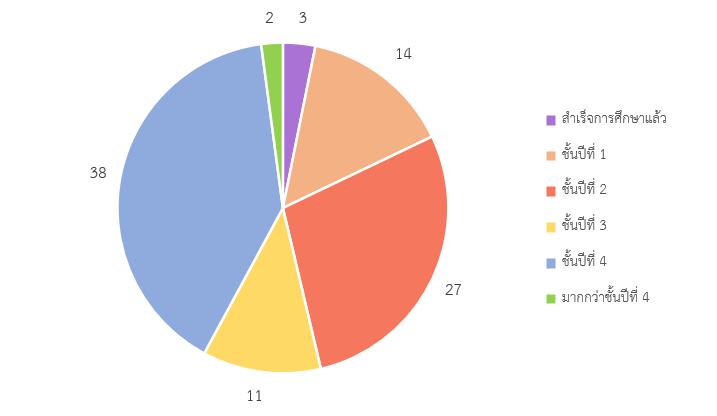
\includegraphics[width=4in]{images/group_by_academic_year.png}
  \end{center}
  \caption[จำนวนผู้ตอบแบบสอบถามแบ่งตามชั้นปีที่ศึกษา]{จำนวนผู้ตอบแบบสอบถามแบ่งตามชั้นปีที่ศึกษา}
  \label{fig:academic_year}     
\end{figure}
และหากแบ่งผู้ตอบแบบสอบถามตามคณะที่ศึกษาจะสามารถแบ่งได้ดังกราฟที่ \ref{fig:faculty} 
โดยคณะอื่น ๆ ประกอบไปด้วยนักศึกษาจากคณะต่าง ๆ ดังนี้
\begin{itemize}
  \item คณะสังคมศาสตร์ จำนวน 2 คน
  \item คณะเกษตรศาสตร์ จำนวน 2 คน
  \item คณะเภสัชศาสตร์ จำนวน 1 คน
  \item คณะเทคนิคการแพทย์ จำนวน 2 คน
  \item คณะพยาบาลศาสตร์ จำนวน 1 คน
  \item คณะสัตวแพทยศาสตร์ จำนวน 2 คน
  \item คณะรัฐศาสตร์และรัฐประศาสนศาสตร์ จำนวน 1 คน
  \item วิทยาลัยศิลปะ สื่อ และเทคโนโลยี จำนวน 1 คน
\end{itemize}
\begin{figure}
  \begin{center}
    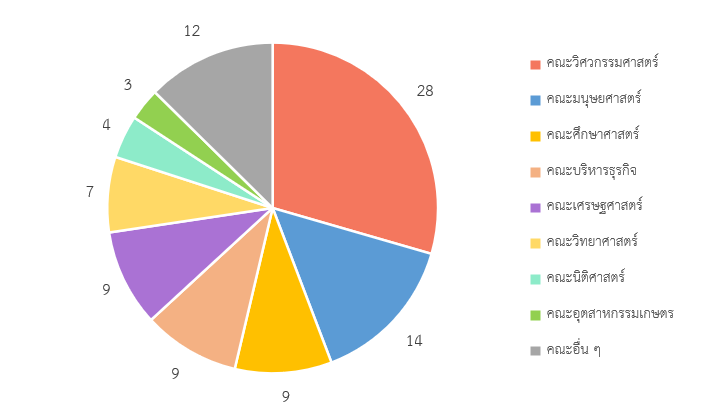
\includegraphics[width=\linewidth]{images/group_by_faculty.png}
  \end{center}
  \caption[จำนวนผู้ตอบแบบสอบถามแบ่งตามคณะที่ศึกษา]{จำนวนผู้ตอบแบบสอบถามแบ่งตามคณะที่ศึกษา}
  \label{fig:faculty}     
\end{figure}

จากการสรุปผลการสำรวจ กราฟที่ \ref{fig:check_before_enrollment} แสดงให้เห็นว่าผู้ตอบแบบสอบถามส่วนใหญ่นั้นตรวจสอบตารางสอบของทุกวิชาที่ต้องการจะลงทะเบียน
ก่อนที่จะลงทะเบียนเรียนอย่างสม่ำเสมอ แต่ยังมีผู้ตอบแบบสอบถามบางส่วนที่ตรวจสอบตารางสอบเพียงบางวิชาก่อนจะลงทะเบียนเรียน และยังมีมีผู้ตอบแบบสอบถามส่วนน้อยที่ตอบว่าไม่เคยตรวจสอบตารางสอบของตนเองเลย
จากกราฟที่ \ref{fig:registration_exam} เรายังพบอีกว่า กลุ่มสำรวจกว่า 80\% ไม่ทราบว่าสำนักทะเบียนและประมวลผล มหาลัยเชียงใหม่ จัดตารางสอบปลายภาคให้กับแต่ละวิชาอย่างไร
\begin{figure}
  \begin{center}
    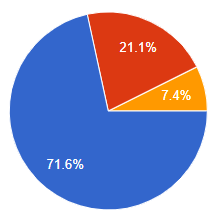
\includegraphics{images/checking_schedule_before_enrollment.png}\\[2ex]
    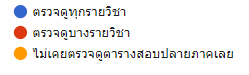
\includegraphics{images/legend_for_checking_schedule_before_enrollment.png}
  \end{center}
  \caption[จำนวนผู้ตอบแบบสอบถามที่ตรวจสอบตารางสอบปลายภาคก่อนการลงทะเบียน]{จำนวนผู้ตอบแบบสอบถามที่ตรวจสอบตารางสอบปลายภาคก่อนการลงทะเบียน}
  \label{fig:check_before_enrollment}     
\end{figure}
\begin{figure}
  \begin{center}
    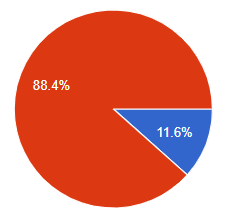
\includegraphics{images/registration_exam.png}\\[2ex]
    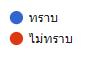
\includegraphics{images/legend_for_registration_exam.png}
  \end{center}
  \caption[จำนวนผู้ตอบแบบสอบถามที่ทราบวิธีการจัดตารางสอบปลายภาคของสำนักทะเบียน]{จำนวนผู้ตอบแบบสอบถามที่ทราบวิธีการจัดตารางสอบปลายภาคของสำนักทะเบียน}
  \label{fig:registration_exam}     
\end{figure}

จากกราฟที่ \ref{fig:time} เราสามารถบอกได้ว่าเวลาที่ผู้ตอบแบบสอบถามส่วนใหญ่ต้องการที่จะสอบในแต่ละวันคือ
ช่วงเวลา 12.00--15.00 ซึ่งผู้ตอบแบบสอบถามส่วนมากต้องการจะสอบช่วงเวลานี้มากกว่า 15.30--18.00 และ 08.00--11.00 ตามลำดับ
\begin{figure}
  \begin{center}
    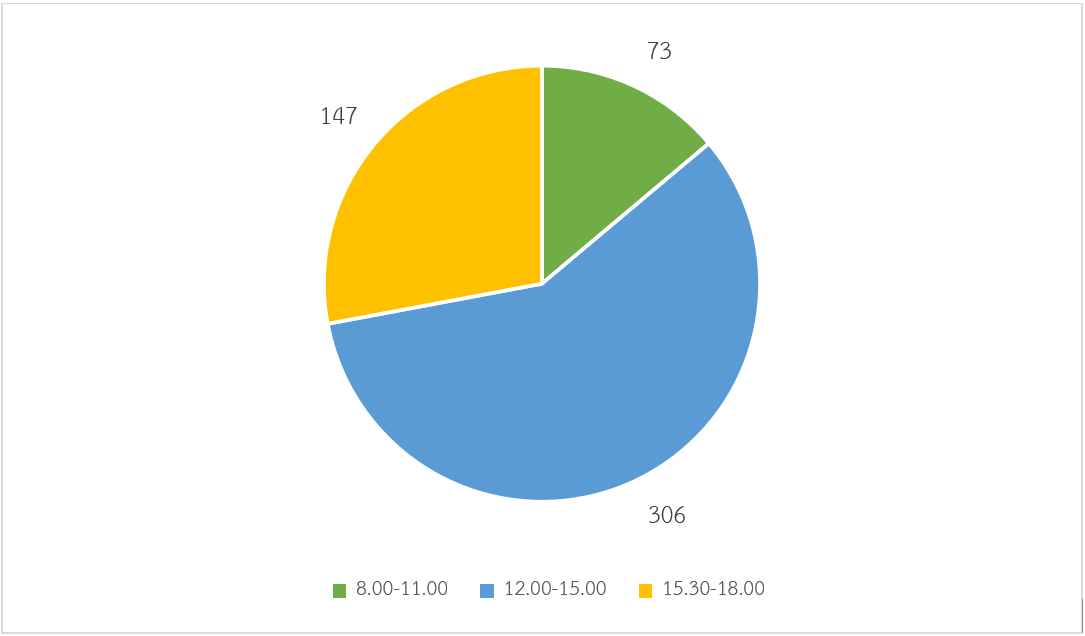
\includegraphics[width=\linewidth]{images/pie_chart_for_final_exam_time.png}
  \end{center}
  \caption{ความต้องการในการสอบของผู้ตอบแบบสอบถามในแต่ละเวลา}
  \label{fig:time}
\end{figure}
และจากกราฟที่ \ref{fig:time_slot} เราทำการรวมช่วงเวลาที่ผู้ตอบแบบสอบถามต้องการสอบกับวันที่ผู้ตอบแบบสอบถามต้องการสอบเข้าด้วยกัน ซึ่งจะสามารถสรุป slot ที่ผู้ตอบแบบสอบถามต้องการจะสอบมากที่สุด 7 อันดับแรก โดยเรียงลำดับจากมากไปน้อยได้ ดังนี้
\begin{figure}
  \begin{center}
    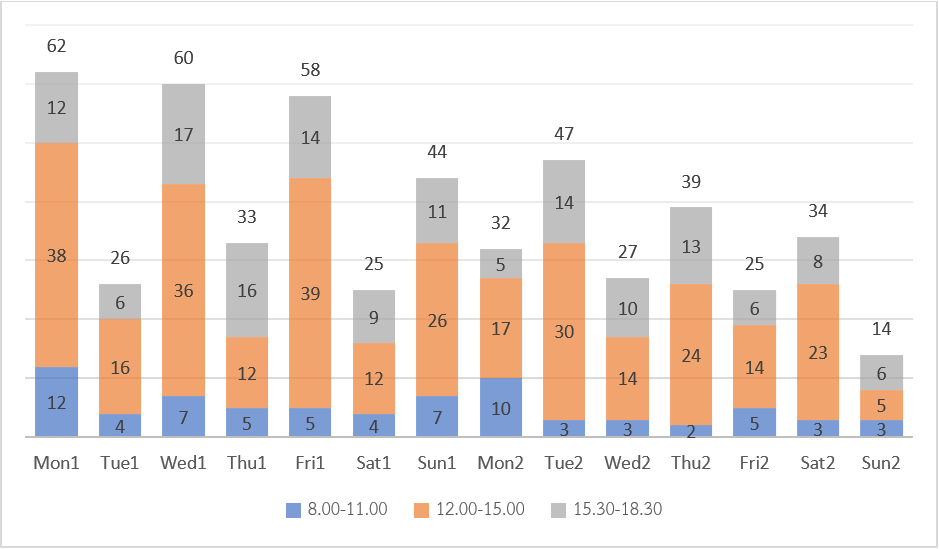
\includegraphics[width=\linewidth]{images/bar_chart_for_final_exam_slot.png}
  \end{center}
  \caption[ความต้องการในการสอบของผู้ตอบแบบสอบถามในแต่ละช่วงเวลาสอบ]{ความต้องการในการสอบของผู้ตอบแบบสอบถามในแต่ละช่วงเวลาสอบ}
  \label{fig:time_slot}     
\end{figure}
\begin{enumerate}
  \item สัปดาห์ที่หนึ่ง เวลา 12.00-15.00น. วันศุกร์ 
  \item สัปดาห์ที่หนึ่ง เวลา 12.00-15.00น. วันจันทร์
  \item สัปดาห์ที่หนึ่ง เวลา 12.00-15.00น. วันพุธ
  \item สัปดาห์ที่สอง เวลา 12.00-15.00น. วันอังคาร
  \item สัปดาห์ที่หนึ่ง เวลา 12.00-15.00น. วันอาทิตย์
  \item สัปดาห์ที่สอง เวลา 12.00-15.00น. วันพฤหัสบดี
  \item สัปดาห์ที่สอง เวลา 12.00-15.00น. วันเสาร์
\end{enumerate}

แต่หากเราตัดเรื่องเวลาที่สอบออก เรายังสามารถสรุปวันที่ผู้ทำแบบสอบถามต้องการจะสอบมากที่สุด 7 อันดับแรก โดยเรียงลำดับจากมากไปน้อย ดังนี้
\begin{enumerate}
  \item สัปดาห์ที่หนึ่ง วันจันทร์
  \item สัปดาห์ที่หนึ่ง วันพุธ
  \item สัปดาห์ที่หนึ่ง วันศุกร์ 
  \item สัปดาห์ที่หนึ่ง วันอาทิตย์
  \item สัปดาห์ที่สอง วันอังคาร
  \item สัปดาห์ที่สอง วันพฤหัสบดี
  \item สัปดาห์ที่สอง วันเสาร์
\end{enumerate}
ซึ่งจากกราฟ \ref{fig:time_slot} ยังสามารถสรุปได้ว่าผู้ตอบแบบสอบถามส่วนใหญ่ต้องการที่จะสอบหนึ่งวันเว้นหนึ่งวันเพื่อที่จะได้มีเวลาในการอ่านหนังสือเตรียมสอบสำหรับวิชาในวันถัดไปมากกว่าการสอบติดกัน 
เรายังสามารถบอกเพิ่มเติมได้อีกว่าผู้ตอบแบบสอบถามส่วนใหญ่ต้องการสอบในช่วงสัปดาห์แรกของช่วงการสอบมากกว่าช่วงสัปดาห์ที่สองเพื่อที่จะได้มีเวลาพักผ่อนหรือกลับบ้าน หลังจากที่สอบเสร็จแล้ว

\subsection{การเก็บข้อมูลตารางสอบ}
หลังจากได้ผลการสำรวจแล้วเราจึงได้ออกสำรวจเพื่อเก็บข้อมูลต่าง ๆ ที่จำเป็นต้องใช้ในการจัดตารางสอบปลายภาค และใช้ในการประเมินผลตารางสอบปลายภาค 
โดยในส่วนของการเก็บข้อมูลเราได้มีการเก็บข้อมูลโดยแบ่งเป็น 2 ส่วนใหญ่ ๆ คือ การเก็บข้อมูลตารางสอบของสำนักทะเบียน และ การเก็บข้อมูลรายวิชาที่มีการจัดสอบและห้องสอบของแต่ละคณะ


ในส่วนของการเก็บข้อมูลตารางสอบของสำนักทะเบียนนั้นเราจะต้องทำการเก็บข้อมูลวิชาที่จัดสอบแบบ special exam ซึ่งสามารถดูรายชื่อวิชาได้จากเว็บสำนักทะเบียนและประมวลผล มหาวิทยาลัยเชียงใหม่ โดยตรง
และเก็บข้อมูลวิชาที่จัดสอบแบบ Regular Exam โดยการส่ง request ผ่าน API เพื่อขอข้อมูลวันและเวลาที่จัดการเรียนการสอนเพื่อนำมาใช้ mapping กับตารางสอบแบบ Regular Exam เพื่อแปลงไปเป็นวันและเวลาสอบปลายภาค
ซึ่งในระหว่างการเก็บข้อมูลเราได้พบปัญหาที่ทำให้การนำข้อมูลไปใช้งานเลยตรง ๆ ทำได้ยาก โดยมีปัญหาอยู่ 2 ประการ (ก) เป็นปัญหาที่ระบบการเก็บข้อมูลของสำนักทะเบียนและประมวลผล มหาวิทยาลัยเชียงใหม่ 
ไม่ได้มีการตรวจสอบความถูกต้องของรูปแบบข้อมูล เมื่อมีการแก้ไขข้อมูลวันและเวลาเรียนของแต่ละวิชา ซึ่งอาจเป็นการแก้ไขด้วยการกรอกวันและเวลาเรียนโดยเจ้าหน้าที่ที่เกี่ยวข้อง ซึ่งบางวิชามีการแสดงผลเวลาเรียนผิดพลาดไปจากรูปแบบปกติ
เช่นในบางวิชาที่มีเวลาเรียนคือ 0930--1100 แต่เวลาที่เขียนกลับเป็น 9030--1100 หรือในบางวิชาเขียนเป็น 9.30-1100 (ข) ในบางวิชาที่เขียนว่าจัดสอบแบบ Regular Exam แต่มีวันและเวลาเรียนไม่ตรงกับรูปแบบใดเลยในตารางสอบแบบ Regular Exam
เช่นมีวันที่เรียนเป็นวันเสาร์--อาทิตย์ หรือ มีเวลาเริ่มเรียน 0900 เป็นต้น \TSNAreply{อาจจะแนบรูปวิชาเหล่านั้นได้ถ้าหาเจอ - -}


ในส่วนของเก็บข้อมูลรายวิชาต่าง ๆ ที่มีการจัดสอบจากแต่ละคณะ เราได้เขียนบันทึกข้อความคำร้องขอข้อมูลไปยังแต่ละคณะ ตัวอย่างดังรูปที่~\ref{fig:request-memo-scan} 
ซึ่งข้อมูลที่ต้องการใช้งาน ได้แก่ ข้อมูลห้องที่สามารถจัดสอบได้พร้อมจำนวนนักศึกษาที่จุได้ในแต่ละห้องของแต่ละคณะ และข้อมูลตารางสอบปลายภาคของแต่ละคณะ เป็นเวลา 3 ปีย้อนหลัง
ซึ่งทางเราได้ตั้งสมมติฐานว่า วิชาใดที่มีรายชื่อวิชาอยู่ในคำสั่งแต่งตั้งกรรมการคุมสอบของแต่ละคณะนั้น จะมีการจัดสอบปลายภาคขึ้นจริง ๆ โดยในแต่ละคณะมีระยะเวลาในการค้นหา รวบรวมและจัดส่งข้อมูลไม่เท่ากัน
ซึ่งเราได้ใช้เวลาร่วมเดือนในการเก็บข้อมูลให้ได้ครบทั้ง 20 คณะและวิทยาลัยศิลปะ สื่อ และเทคโนโลยี
\begin{figure}
  \begin{center}
    
\includegraphics[width=\linewidth]{images/request_memo_scan_crop.png}
  \end{center}
  \caption[ตัวอย่างใบบันทึกข้อความเพื่อขอข้อมูลตารางสอบ]{ตัวอย่างใบบันทึกข้อความเพื่อขอข้อมูลตารางสอบ}
  \label{fig:request-memo-scan}     
\end{figure}
\CIreply{ใส่รูปสแกนบันทึกข้อความของสักคณะ}

\section{โครงสร้างและการทำงานของโปรแกรม}

\subsection{รูปแบบของผลลัพธ์จากการจัดตารางสอบ}
ข้อมูลผลลัพธ์ของโปรแกรมจะเป็นไฟล์ CSV ที่ระบุรายวิชาคู่กับหมายเลข slot ที่สอบของรายวิชานั้น ๆ โดยจะมีข้อมูลใช้สำหรับ mapping หมายเลข slot เป็นวันและเวลาสอบ
โดยหมายเลข slot แต่ละหมายเลขจะบ่งบอกถึงวันและเวลาสอบที่ต่างกันในแต่ละภาคการศึกษา

\subsection{การออกแบบอัลกอริทึมและแผนผังการทำงานของโปรแกรม}
ในการออกแบบอัลกอริทึมสำหรับใช้ในการจัดตารางสอบ จะใช้วิธีการระบายสีกราฟ (graph coloring) 
โดยจะแปลงรายวิชาที่ต้องจัดสอบเป็นโหนดของกราฟ (node) 
และคู่วิชาที่มีนักศึกษาคนใด ๆ ลงทะเบียนพร้อมกันในภาคการศึกษานั้นจะถูกจัดให้สอบพร้อมกันไม่ได้ 
จึงจะถูกแปลงเป็นเส้นเชื่อมในกราฟ (edge) จำนวนนักศึกษาที่ลงทะเบียนในคู่วิชานั้น ๆ จะถูกแปลงเป็น edge weights
และช่วงเวลาที่แต่ละวิชาจัดสอบ (slot) จะถูกแปลงเป็นสีของโหนด
สำหรับแต่ละโหนด เราจะนิยาม \emph{degree of conflicts} เป็นผลรวมของ weights จากทุกๆ edge ที่ต่ออยู่กับโหนดนั้นๆ
และเรียกจำนวนเส้นเชื่อมทั้งหมดที่เข้า--ออก จากกราฟว่า\emph{ดีกรี} (degree) 
โดยอัลกอริทึมจะมีลำดับการทำงานตามรูปที่ \ref{fig:flowchart} 
โดยเมื่อจะรันโปรแกรมจะต้องเลือกอัลกอริทึมรูปแบบใดรูปแบบหนึ่ง จากทั้งหมด 4 รูปแบบ ดังขั้นตอนที่ 1
และอัลกอริทึมจะมีรูปแบบการทำงานทั้งหมด 4 รูปแบบ โดยแต่ละรูปแบบจะมีความแตกต่างกันที่ลำดับการเลือกโหนดมาเพื่อละบายสี
โดยแต่ละรูปแบบจะมีการเรียงลำดับ ดังตอนที่ \ref{subsec:sorting_type}

\subsection{รูปแบบของอัลกอริทึม}
\label{subsec:sorting_type}
\begin{enumerate}
  \item รูปแบบที่ 1 BFS-DEG: ทำ BFS จากแต่ละโหนดโดยมีการเรียงลำดับความสำคัญของโหนดที่จะจัดช่วงเวลาสอบก่อน โดยเรียงจาก
  ดีกรีของโหนด จำนวนนักศึกษาที่ลงทะเบียน จำนวน conflict ของโหนด และหากทุกอย่างเท่ากันจะเรียงตามรหัสวิชา โดยเรียงจากมากไปน้อยตามลำดับ
  เมื่อจัดช่วงเวลาสอบให้ครบทุกโหนดเพื่อนบ้านแล้วจะเริ่มกระบวนการนี้ซ้ำที่โหนดเพื่อนบ้านถัดไป จนกว่าจะจัดช่วงเวลาสอบได้ครบทุกโหนด
  \item รูปแบบที่ 2 DEG: จัดช่วงเวลาสอบให้แต่ละโหนดโดยมีการเรียงลำดับความสำคัญของโหนดที่จะจัดช่วงเวลาสอบก่อน โดยเรียงจาก
  ดีกรีของโหนด จำนวนนักศึกษาที่ลงทะเบียน จำนวน conflict ของโหนด และหากทุกอย่างเท่ากันจะเรียงตามรหัสวิชา โดยเรียงจากมากไปน้อยตามลำดับ
  \item รูปแบบที่ 3 BFS-STD: ทำ BFS จากแต่ละโหนดโดยมีการเรียงลำดับความสำคัญของโหนดที่จะจัดช่วงเวลาสอบก่อน โดยเรียงจาก
  จำนวนนักศึกษาที่ลงทะเบียน ดีกรีของโหนด จำนวน conflict ของโหนด และหากทุกอย่างเท่ากันจะเรียงตามรหัสวิชา โดยเรียงจากมากไปน้อยตามลำดับ
  เมื่อจัดช่วงเวลาสอบให้ครบทุกโหนดเพื่อนบ้านแล้วจะเริ่มกระบวนการนี้ซ้ำที่โหนดเพื่อนบ้านถัดไป จนกว่าจะจัดช่วงเวลาสอบได้ครบทุกโหนด
  \item รูปแบบที่ 4 STD: จัดช่วงเวลาสอบให้แต่ละโหนดโดยมีการเรียงลำดับความสำคัญของโหนดที่จะจัดช่วงเวลาสอบก่อน โดยเรียงจาก
  จำนวนนักศึกษาที่ลงทะเบียน ดีกรีของโหนด จำนวน conflict ของโหนด และหากทุกอย่างเท่ากันจะเรียงตามรหัสวิชา โดยเรียงจากมากไปน้อยตามลำดับ
\end{enumerate}

\begin{figure}
  \begin{center}
    \begin{tikzpicture}[flowchart]
      \node[startstop] (start) {start};
      \node[io] (a) [below=0.4cm of start] {{เลือกรูปแบบการทำงานของอัลกอริทึมจากทั้งหมด 4 รูปแบบ}};
      \node[io2] (b) [below=0.4cm of a] {{
        \begin{minipage}{4.25in}
        \begin{itemize}[nosep]
        \item อ่านข้อมูลลงทะเบียนของนักศึกษาแต่ละคน
        \item อ่านข้อมูลรายวิชาทั้งหมดที่มีนักศึกษาลงทะเบียน
        \item อ่านข้อมูลคู่รายวิชาที่มีนักศึกษาลงทะเบียนทั้งสองวิชาอย่างน้อย 1 คน (conflicts)
        \item อ่านข้อมูลรายวิชาทั้งหมดที่มีการจัดสอบ
        \item อ่านข้อมูลรายวิชาของแต่คณะ
        \item อ่านข้อมูลจำนวนความจุของที่นั่งสอบของแต่ละคณะ
      \end{itemize}        
      \end{minipage}    
      }};
      \node[process] (proa) [below=0.4cm of b ] {
        \begin{minipage}{3.6in}
          คัดกรองรายวิชาที่ต้องจัดสอบให้เหลือเพียงรายวิชาที่มีนักศึกษาลงทะเบียนและเป็นรายวิชาที่มีอยู่ในลิสต์ของรายวิชาที่มีการจัดสอบ
        \end{minipage}    
        };
      \node[process] (prob) [below=0.4cm of proa] {
      \begin{minipage}{3.7in}
        สร้างกราฟ
        \begin{itemize}[nosep]
        \item เพิ่ม nodes ของกราฟจากรายวิชาที่ได้จากขั้นตอนก่อนหน้า
        \item เพิ่ม edges ของแต่ละ nodes ตามคู่รายวิชาที่มี conflicts
      \end{itemize}        
      \end{minipage}                      
      };
      \node[connector] (con) [below=0.4cm of prob] {};
      \node[decision] (desa) [below=0.4cm of con] {visit ครบทุก node?};
      \node[process] (prod) [below=0.4cm of desa] {เลือก node ถัดไป};
      \node[process] (proe) [below=0.4cm of prod] {
        \begin{minipage}{4.3in}
          จัดตารางสอบให้ node ปัจจุบัน โดยทดลองทุก slot ที่จัดสอบได้และเลือก slot ที่ทำให้ค่า penalty น้อยที่สุดตาม penalty model 
        \end{minipage} 
      };
      \node[process] (prof) [below=0.2cm of proe] {คิดคำนวณค่า penalty ของตารางสอบ};
      \node[io] (c) [below=0.4cm of prof] {
        \begin{minipage}{3.7in}
          \begin{itemize}[nosep]
          \item แสดงค่า penalty ของตารางสอบ
          \item เขียนผลลัพธ์ของตารางสอบและค่า penalty ลงในไฟล์
        \end{itemize}        
        \end{minipage}  };
      \node[startstop] (end) [below=0.4cm of c] {end};
      
      \draw[arrow] (start) -- (a);
      \draw[arrow] (a) -- (b);
      \draw[arrow] (b) -- (proa);
      \draw[arrow] (proa) -- (prob);
      \draw[arrow] (prob) -- (con);
      \draw[arrow] (con) -- (desa);
      \draw[arrow] (desa) -- node[near start,right]{False} (prod);
      \draw[arrow] (desa.east) -- node[near start,above]{True} +(4cm,0) |- (prof);
      \draw[arrow] (prod) -- (proe);
      \draw[arrow] (proe.west) -- +(-0.5cm,0) |- (con);
      \draw[arrow] (prof) -- (c);
      \draw[arrow] (c) -- (end);
            
    \end{tikzpicture}
  \end{center}
  \caption[แผนผังการทำงานของโปรแกรม]{แผนผังการทำงานของโปรแกรม}
  \label{fig:flowchart}     
\end{figure}
\CIreply{เรายังต้องทำตาม component จริงหรือ? หรือแค่ทำจนครบทุก node เรียงลำดับตามวิธีที่เราเลือกใช้?}
\TSNAreply{ถ้าใช้ BFS ต้องแยก component เพราะไม่งั้นจะ visit ไม่ครบทุก node แต่ถ้าไม่ใช้ BFS น่าจะไม่ต้องตาม component ได้ครับ}

\chapter{\ifproject%
\ifcpe การทดลองและผลลัพธ์\else Experimentation and Results\fi
\else%
\ifcpe การประเมินระบบ\else System Evaluation\fi
\fi}

การประเมินระบบสำหรับโครงงานนี้จะเน้นไปที่การคำนวณค่าความเหมาะสมของตารางสอบที่ได้จากระบบ เพื่อเปรียบเทียบกับตารางสอบที่กำหนดโดยสำนักทะเบียนและประมวลผล 
\enskip การคำนวณค่าความเหมาะสมของตารางสอบที่ได้นั้นจะคำถึงนึงคุณสมบัติของตารางสอบตามวัตถุประสงค์ของโครงงาน ดังที่ได้ระบุไว้ในตอนที่~\ref{sec:Objectives} 
โดยสามารถประเมินความเหมาะสมได้ 2 วิธี กล่าวคือ การนับจำนวนครั้งที่ตารางสอบสำหรับนักศึกษาคนใดๆ ไม่เป็นไปตามที่พึงประสงค์ และการสอบถามความพึงพอใจของนักศึกษาที่มีต่อตารางสอบที่ได้จากระบบ เพื่อช่วยในการยืนยันว่าตัวชี้วัดที่โปรแกรมใช้คำนวณค่าความเหมาะสมของตารางสอบนั้นสอดคล้องกับความต้องการของผู้ใช้งานอย่างแท้จริง

\section{การประเมินระบบด้วย penalty}
การประเมินผลระบบจัดตารางสอบที่จะพัฒนาขึ้นมานั้นจะพิจารณาปัจจัยด้านความสมดุลและความเหมาะสมของตารางสอบที่ได้ โดยสามารถกำหนดค่าอันไม่พึงประสงค์ (penalty) ของตารางสอบแต่ละแบบที่เป็นผลลัพธ์จากระบบ
\enskip ตารางสอบที่มีความเหมาะสมมาก ควรจะมี penalty น้อย
\enskip นอกจากจะมีการคำนวณ penalty เพื่อเปรียบเทียบตารางสอบแบบต่างๆ ที่ได้จากระบบแล้ว การคำนวณในลักษณะเดียวกันนี้จะใช้กับตารางสอบดั้งเดิมดังที่ได้กำหนดโดยสำนักทะเบียนและประมวลผลอีกด้วย เพื่อยืนยืนว่าตารางสอบที่ได้จากระบบนั้นมีคุณภาพดีกว่าตารางสอบที่มีอยู่เดิม

\subsection{การคำนวณ penalty}
Penalty ของตารางสอบแต่ละแบบที่ได้จากระบบนั้น คำนวณได้จากค่า penalty ของการที่มีนักศึกษาที่สอบในช่วงเวลาใด ๆ ที่เกินกว่าจํานวนที่นั่งสอบที่ทางมหาวิทยาลัยสามารถจัดให้ได้
รวมกับค่า penalty ของตารางสอบสำหรับนักศึกษารายบุคคล ว่ามีความเหมาะสมกับนักศึกษารายนั้นๆ มากน้อยเพียงใด 
โดยการคิดค่า penalty ของนักศึกษาแต่ละคนนั้น จะใช้ตัวชี้วัดทั้งสิ้น 6 แบบ ตามลำดับที่ 2--7 ซึ่งมีน้ำหนักแตกต่างกันไปตามความไม่พึงประสงค์ที่สรุปได้จากผลสำรวจในตอนที่~\ref{sec:collecting_data} 
โดยคิดจากสัดส่วนนักศึกษาที่ไม่ชอบให้เกิดสถานการณ์ดังกล่าว ซึ่งได้กำหนดให้มีค่า Penalty ของสถานการณ์ต่าง ๆ ที่เกิดขึ้นในตารางสอบของนักศึกษาแต่ละคน เรียงตามน้ำหนักจากมากไปน้อยได้ดังนี้
  
\begin{enumerate}
    \item จํานวนนักศึกษาเกินความจุที่นั่งสอบของคณะ มีการคิดค่า penalty ตามสมการที่จะกล่าวต่อไป
    \item มีนักศึกษาคนใด ๆ ถูกกำหนดให้สอบสองวิชาในเวลาเดียวกัน ครั้งละ 10000 Points
    \item มีนักศึกษาคนใด ๆ ถูกกำหนดให้สอบเวลา 8.00--11.00\,น. และ 12.00--15.00\,น. ในวันเดียวกัน ครั้งละ 78 Points
    \item มีนักศึกษาคนใด ๆ ถูกกำหนดให้สอบเวลา 12.00--15.00\,น. และ 15.30--18.30\,น. ในวันเดียวกัน ครั้งละ 78 Points
    \item มีนักศึกษาคนใด ๆ ถูกกำหนดให้สอบเวลา 8.00--11.00\,น. และ 15.30--18.30\,น. ในวันเดียวกัน ครั้งละ 38 Points
    \item มีนักศึกษาคนใด ๆ ถูกกำหนดให้สอบเวลา 15.30--18.30\,น. และ 08.00--11.00\,น. ในวันรุ่งขึ้น ครั้งละ 29 Points
    \item นักศึกษามีวันเว้นว่างระหว่างการสอบสองวิชาที่ติดกันมากกว่า 3 วัน ครั้งละ 12 Points
\end{enumerate}
สำหรับค่า Penalty ที่เกิดจากจำนวนนักศึกษาเกินความจุที่นั่งสอบของคณะในแต่ละช่วงเวลาสอบนั้นจะมีการคิดคำนวณแยกตามคณะดังนี้
\begin{itemize}
    \item หากจัดให้นักศึกษาสอบที่คณะแล้วจำนวนนักศึกษารวมมากกว่า 100\% ของที่นั่งสอบในคณะสำหรับวิชาของคณะนั้น ๆ ในแต่ละช่วงเวลาที่สอบ จะจัดให้นักศึกษาสอบเต็ม 80\% ของที่นั่งคณะ
    หลังจากนั้นจัดให้นักศึกษาที่เกินความจุ 80\% สอบที่ตึกอาคารเรียนรวมเท่าที่จัดได้หากอาคารเรียนรวมยังมีที่นั่งเหลือ แต่หากจัดที่อาคารเรียนรวมแล้วยังมีที่นั่งไม่เพียงพอ จะทำการคิดค่า penalty ของนักศึกษาที่เหลือ
    โดยหากจำนวนนักศึกษาเกินความจุ 80\% ไป แต่ไม่เกิน 100 \% จะคิดตามสมการเส้นตรงดังนี้ 
    \begin{equation}
    \label{eqn:linear}
        f(x)=500(x-80)
    \end{equation}
    หากจำนวนนักศึกษาเกินความจุ 100 \% จะคิดตามสมการเอกซ์โพเนนเชียลดังนี้ 
    \begin{equation}
    \label{eqn:exponential}
        f(x)=500(x-80)+2^{2(\frac{x}{10}-1)}-2^{18}
    \end{equation}
    โดยที่ค่า x คือ เปอร์เซ็นต์ของความจุที่นั่งของคณะที่ใช้ไปแล้ว
    \item หากจัดให้นักศึกษาสอบที่คณะแล้วจำนวนนักศึกษารวมมากกว่า 80\% ของที่นั่งสอบในคณะสำหรับวิชาของคณะนั้น ๆ ในแต่ละช่วงเวลาที่สอบ แต่ไม่เกิน 100\% จะจัดให้นักศึกษาสอบเต็ม 80\% ของที่นั่งคณะ
    หลังจากนั้นจัดให้นักศึกษาที่เกินความจุ 80\% สอบที่ตึกอาคารเรียนรวมเท่าที่จัดได้หากอาคารเรียนรวมยังมีที่นั่งเหลือ แต่หากจัดที่อาคารเรียนรวมแล้วยังมีที่นั่งไม่เพียงพอ จะทำการคิดค่า penalty ของนักศึกษาที่เหลือแต่เกิน 80\% ไป
    โดยคิดตามสมการเส้นตรงที่~\ref{eqn:linear}
    \item หากจัดให้นักศึกษาสอบที่คณะแล้วจำนวนนักศึกษารวมไม่เกิน 80\% ของที่นั่งสอบในคณะสำหรับวิชาของคณะนั้น ๆ ในแต่ละช่วงเวลาที่สอบ จะไม่มีการคิด penalty
    \item สุดท้ายคิด penalty ของอาคารเรียนรวม หากจำนวนนักศึกษารวมที่ต้องสอบที่อาคารเรียนรวมเกิน 80\% แต่ไม่เกิน 100\% จะคิดตามสมการเส้นตรงที่~\ref{eqn:linear} แต่หากจำนวนนักศึกษารวมที่ต้องสอบที่อาคารเรียนรวมเกิน 100\% จะคิดตามสมการเอกซ์โพเนนเชียลที่~\ref{eqn:exponential}
\end{itemize}
ค่า penalty จะค่อย ๆ เพิ่มขึ้นหลังจากจำนวนนักศึกษารวมเกิน 80\% ของที่นั่งสอบขึ้นไป และเริ่มเพิ่มขึ้นอย่างรวดเร็วหากจำนวนนักศึกษาเกิน 100\% ของที่นั่งสอบดังกราฟที่ \ref{fig:penalty_graph}
\begin{figure}
    \begin{center}
      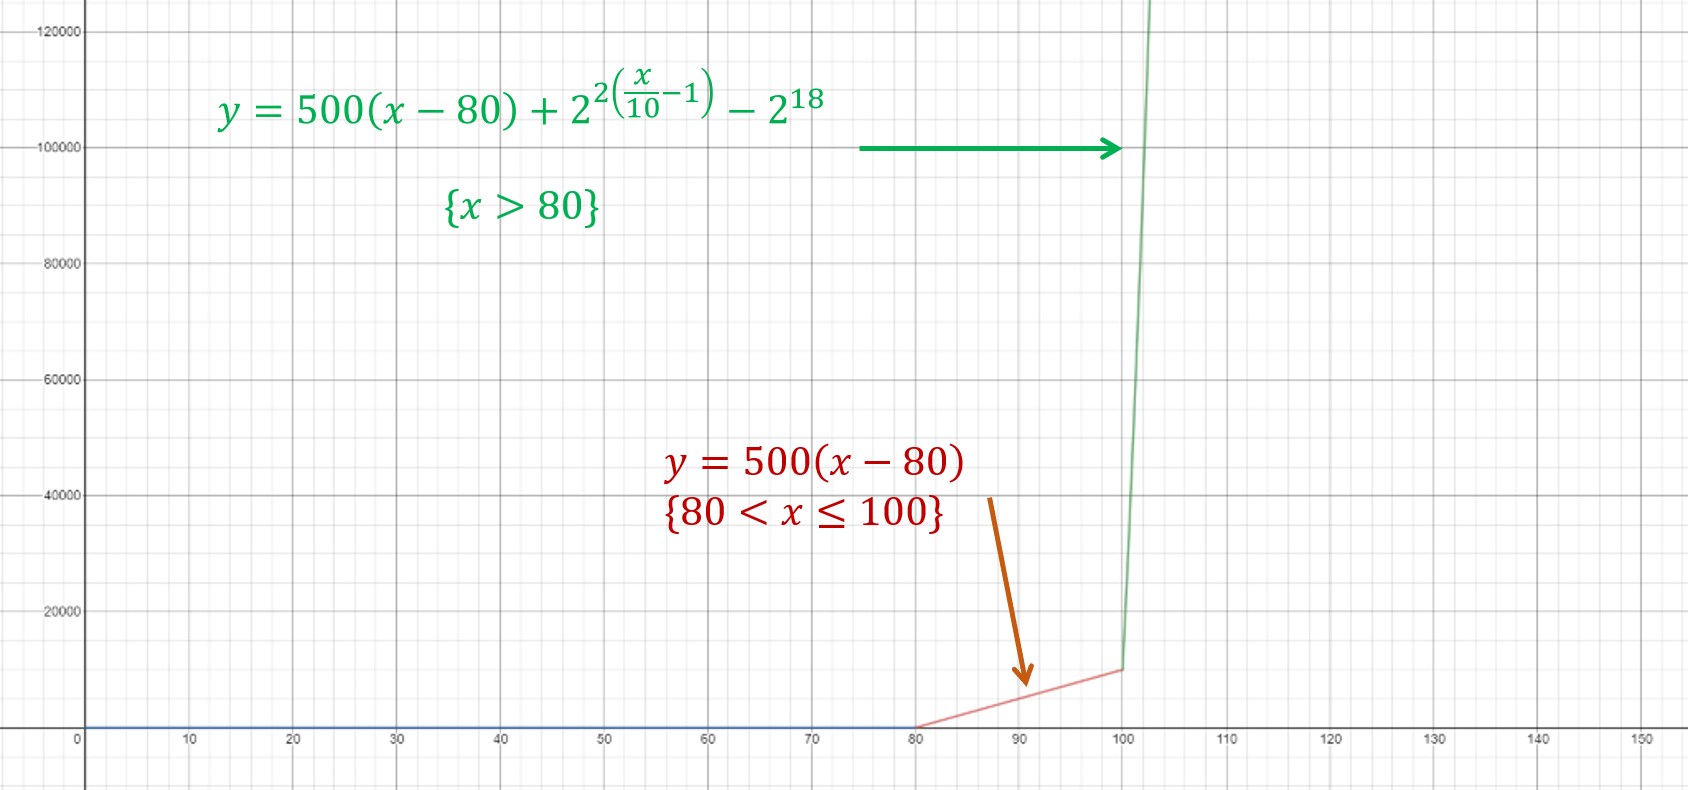
\includegraphics[width=\linewidth]{images/penalty_graph.png}
    \end{center}
    \caption[กราฟแสดงการเพิ่มขึ้นของค่า penalty]{กราฟแสดงการเพิ่มขึ้นของค่า penalty}
    \label{fig:penalty_graph}     
\end{figure}
\newpage
\section{การประเมินระบบโดยสอบถามความพึงพอใจของนักศึกษา}
ตัวชี้วัดที่ใช้ในการคำนวณ penalty ของตารางสอบที่ได้จากระบบนั้น อาจจะไม่ครอบคลุมความพึงประสงค์ทุกรูปแบบจากนักศึกษา หรือน้ำหนักของตัวชี้วัดที่ใช้ในการคำนวณ penalty นั้นอาจจะเป็นไปได้หลายรูปแบบ
\enskip การสอบถามความพึงพอใจของนักศึกษานั้นจะช่วยในการปรับปรุงอัลกอริทึมเพื่อให้สามารถเลือกใช้น้ำหนักของตัวชี้วัดที่เหมาะสมมากขึ้นในการจัดตารางสอบ
อีกทั้งยังช่วยยืนยันว่าตัวชี้วัดที่โปรแกรมใช้คํานวณค่าความเหมาะสมของตารางสอบนั้นสอดคล้องกับความต้องการของผู้ใช้งาน 
\enskip โดยการประเมินระบบด้วยวิธีการนี้ได้มีการทำ A/B Testing โดยได้ออกแบบและสร้างเว็บแอปพลิเคชันให้นักศึกษาผู้ตอบแบบสอบถาม
ล็อกอินผ่าน OAuth ด้วย CMU Account แล้วแสดงข้อมูลตารางสอบของนักศึกษาคนที่ล็อกอิน ภาคการศึกษาละ 2 แบบ เปรียบเทียบกัน 
โดยแบบหนึ่งจะเป็นตารางสอบที่กำหนดโดยสำนักทะเบียนและประมวลผล มหาวิทยาลัยเชียงใหม่ 
อีกแบบหนึ่งจะเป็นตารางสอบที่จัดโดยใช้รูปแบบการเรียงลำดับวิชาในการจัดสอบแบบ DEG จากโปรแกรมจัดตารางสอบ
โดยนักศึกษาจะไม่ทราบว่าตารางสอบที่เห็นแต่ละด้านนั้นเป็นแบบใด จากนั้นจะมีแบบฟอร์มให้นักศึกษาเลือกตารางสอบแบบที่ชอบที่สุด แบ่งเป็น 4 ระดับ ได้แก่ (-2) ชอบแบบ A มากที่สุด (-1) ชอบแบบ A มากกว่าเล็กน้อย (0) ชอบทั้งสองแบบเท่า ๆ กัน (1) ชอบแบบ B มากกว่าเล็กน้อย และ (2) ชอบแบบ B มากที่สุด 
โดยหลังจากนำข้อมูลมาประมวลผลแล้ว เราจะกำหนดให้คะแนนที่ติดลบ [-2,-1] บ่งชี้ความพึงพอใจมากกว่าต่อตารางสอบที่กำหนดโดยสำนักทะเบียนและประมวลผล มหาวิทยาลัยเชียงใหม่
คะแนนที่เป็นบวก [1,2] บ่งชี้ความพึงพอใจมากกว่าต่อตารางสอบจากโปรแกรมจัดตารางสอบ โดยนอกจากจะให้นักศึกษาเลือกระดับความพึงพอใจแล้ว นักศึกษายังต้องให้เหตุผลประกอบกับระดับความพึงพอใจที่ตนเองเลือกด้วย

\newpage
\section{ผลการประเมินระบบด้วย penalty}
การประเมินระบบด้วยค่า penalty นั้นได้มีการจัดตารางสอบทั้งหมด 6 ภาคการศึกษา ตั้งแต่ภาคการศึกษาที่ 1/2561 จนถึงภาคการศึกษาที่ 2/2563
โดยในแต่ละภาคการศึกษาได้มีการทดลองจัดตารางสอบด้วยอัลกอริทึมทั้งหมด 4 รูปแบบ และได้คิดคำนวณจำนวนครั้งที่เกิด penalty และค่า penalty ของตารางสอบแต่ละแบบ ดังตารางที่ \ref{tab:result_table_161} - \ref{tab:result_table_263}
\begin{table}[]
    \centering
    \textbf{Total courses: 1432} \quad \quad \textbf{Total students having an exam: 13171}
    \resizebox{\textwidth}{!}{%
    \begin{tabular}{@{}ccrrrrrrrr@{}}
    \toprule
    \textbf{รูปแบบ}                              & \textbf{Penalty}                      & \textbf{1}                & \textbf{2}               & \textbf{3}                   & \textbf{4}                  & \textbf{5}                  & \textbf{6}                  & \textbf{7}                    & \textbf{รวม}                  \\ \midrule
                                                 & \textbf{Count}                        & 0                         & 0                        & 354                          & 430                         & 1854                        & 171                         & 12930                         & 15739                         \\ \cmidrule(l){2-10} 
    \multirow{-2}{*}{BFS-DEG}                    & \textbf{Value}                        & 0                         & 0                        & 27612                        & 33540                       & 70452                       & 4959                        & 155160                        & 291723                        \\ \midrule
                                                 & \textbf{Count}                        & 1                         & 0                        & 480                          & 140                         & 207                         & 71                          & 12038                         & 12937                         \\ \cmidrule(l){2-10} 
    \multirow{-2}{*}{DEG}                        & \textbf{Value}                        & 21                        & 0                        & 37440                        & 10920                       & 7866                        & 2059                        & 144456                        & 202762                        \\ \midrule
                                                 & \textbf{Count}                        & 1                         & 0                        & 588                          & 210                         & 93                          & 69                          & 10465                         & 11426                         \\ \cmidrule(l){2-10} 
    \multirow{-2}{*}{BFS-STD}                    & \textbf{Value}                        & 2                         & 0                        & 45864                        & 16380                       & 3534                        & 2001                        & 125580                        & 193361                        \\ \midrule
    {\color[HTML]{FE0000} }                      & {\color[HTML]{FE0000} \textbf{Count}} & {\color[HTML]{FE0000} 1}  & {\color[HTML]{FE0000} 0} & {\color[HTML]{FE0000} 431}   & {\color[HTML]{FE0000} 116}  & {\color[HTML]{FE0000} 174}  & {\color[HTML]{FE0000} 60}   & {\color[HTML]{FE0000} 8334}   & {\color[HTML]{FE0000} 9116}   \\ \cmidrule(l){2-10} 
    \multirow{-2}{*}{{\color[HTML]{FE0000} STD}} & {\color[HTML]{FE0000} \textbf{Value}} & {\color[HTML]{FE0000} 64} & {\color[HTML]{FE0000} 0} & {\color[HTML]{FE0000} 33618} & {\color[HTML]{FE0000} 9048} & {\color[HTML]{FE0000} 6612} & {\color[HTML]{FE0000} 1740} & {\color[HTML]{FE0000} 100008} & {\color[HTML]{FE0000} 151090} \\ \bottomrule
    \end{tabular}%
    }
    \caption{ตารางแสดงค่า penalty ของตารางสอบเทอม 1/2561}
    \label{tab:result_table_161}
\end{table}
\begin{table}[]
    \centering
    \textbf{Total courses: 1551} \quad \quad \textbf{Total students having an exam: 13095}
    \resizebox{\textwidth}{!}{%
    \begin{tabular}{@{}ccrrrrrrrr@{}}
    \toprule
    \textbf{รูปแบบ}                              & \textbf{Penalty}                      & \textbf{1}                  & \textbf{2}               & \textbf{3}                   & \textbf{4}                   & \textbf{5}                   & \textbf{6}                  & \textbf{7}                    & \textbf{รวม}                  \\ \midrule
                                                 & \textbf{Count}                        & 1                           & 0                        & 1050                         & 583                          & 296                          & 314                         & 10977                         & 13221                         \\ \cmidrule(l){2-10} 
    \multirow{-2}{*}{BFS-DEG}                    & \textbf{Value}                        & 2467                        & 0                        & 81900                        & 45474                        & 11248                        & 9106                        & 131724                        & 281919                        \\ \midrule
                                                 & \textbf{Count}                        & 1                           & 0                        & 884                          & 264                          & 398                          & 242                         & 12158                         & 13947                         \\ \cmidrule(l){2-10} 
    \multirow{-2}{*}{DEG}                        & \textbf{Value}                        & 238                         & 0                        & 68952                        & 20592                        & 15124                        & 7018                        & 145896                        & 257820                        \\ \midrule
                                                 & \textbf{Count}                        & 1                           & 0                        & 1343                         & 374                          & 742                          & 208                         & 10342                         & 13010                         \\ \cmidrule(l){2-10} 
    \multirow{-2}{*}{BFS-STD}                    & \textbf{Value}                        & 2                           & 0                        & 104754                       & 29172                        & 28196                        & 6032                        & 124104                        & 292260                        \\ \midrule
    {\color[HTML]{FE0000} }                      & {\color[HTML]{FE0000} \textbf{Count}} & {\color[HTML]{FE0000} 1}    & {\color[HTML]{FE0000} 0} & {\color[HTML]{FE0000} 814}   & {\color[HTML]{FE0000} 247}   & {\color[HTML]{FE0000} 266}   & {\color[HTML]{FE0000} 203}  & {\color[HTML]{FE0000} 9649}   & {\color[HTML]{FE0000} 11180}  \\ \cmidrule(l){2-10} 
    \multirow{-2}{*}{{\color[HTML]{FE0000} STD}} & {\color[HTML]{FE0000} \textbf{Value}} & {\color[HTML]{FE0000} 2251} & {\color[HTML]{FE0000} 0} & {\color[HTML]{FE0000} 63492} & {\color[HTML]{FE0000} 19266} & {\color[HTML]{FE0000} 10108} & {\color[HTML]{FE0000} 5887} & {\color[HTML]{FE0000} 115788} & {\color[HTML]{FE0000} 216792} \\ \bottomrule
    \end{tabular}%
    }
    \caption{ตารางแสดงค่า penalty ของตารางสอบเทอม 2/2561}
    \label{tab:result_table_261}
\end{table}
\begin{table}[]
    \centering
    \textbf{Total courses: 1729} \quad \quad \textbf{Total students having an exam: 19786}
    \resizebox{\textwidth}{!}{%
    \begin{tabular}{@{}ccrrrrrrrr@{}}
    \toprule
    \textbf{รูปแบบ}                              & \textbf{Penalty}                      & \textbf{1}                  & \textbf{2}               & \textbf{3}                   & \textbf{4}                   & \textbf{5}                   & \textbf{6}                  & \textbf{7}                    & \textbf{รวม}                  \\ \midrule
                                                 & \textbf{Count}                        & 0                           & 0                        & 1110                         & 657                          & 1217                         & 639                         & 18036                         & 21659                         \\ \cmidrule(l){2-10} 
    \multirow{-2}{*}{BFS-DEG}                    & \textbf{Value}                        & 0                           & 0                        & 86580                        & 51246                        & 46246                        & 18531                       & 216432                        & 419035                        \\ \midrule
                                                 & \textbf{Count}                        & 1                           & 0                        & 1155                         & 242                          & 522                          & 147                         & 18859                         & 20926                         \\ \cmidrule(l){2-10} 
    \multirow{-2}{*}{DEG}                        & \textbf{Value}                        & 714                         & 0                        & 90090                        & 18876                        & 19836                        & 4263                        & 226308                        & 360087                        \\ \midrule
                                                 & \textbf{Count}                        & 1                           & 0                        & 1500                         & 595                          & 259                          & 159                         & 15990                         & 18504                         \\ \cmidrule(l){2-10} 
    \multirow{-2}{*}{BFS-STD}                    & \textbf{Value}                        & 2                           & 0                        & 117000                       & 46410                        & 9842                         & 4611                        & 191880                        & 369745                        \\ \midrule
    {\color[HTML]{FE0000} }                      & {\color[HTML]{FE0000} \textbf{Count}} & {\color[HTML]{FE0000} 3}    & {\color[HTML]{FE0000} 0} & {\color[HTML]{FE0000} 965}   & {\color[HTML]{FE0000} 334}   & {\color[HTML]{FE0000} 337}   & {\color[HTML]{FE0000} 231}  & {\color[HTML]{FE0000} 15535}  & {\color[HTML]{FE0000} 17405}  \\ \cmidrule(l){2-10} 
    \multirow{-2}{*}{{\color[HTML]{FE0000} STD}} & {\color[HTML]{FE0000} \textbf{Value}} & {\color[HTML]{FE0000} 4259} & {\color[HTML]{FE0000} 0} & {\color[HTML]{FE0000} 75270} & {\color[HTML]{FE0000} 26052} & {\color[HTML]{FE0000} 12806} & {\color[HTML]{FE0000} 6699} & {\color[HTML]{FE0000} 186420} & {\color[HTML]{FE0000} 311506} \\ \midrule
                                                 & \textbf{Count}                        & 0                           & 3247                     & 3406                         & 2333                         & 7663                         & 5863                        & 18667                         & 41179                         \\ \cmidrule(l){2-10} 
    \multirow{-2}{*}{สำนักทะเบียน}                  & \textbf{Value}                        & 0                           & 32470000                 & 265668                       & 181974                       & 291194                       & 170027                      & 224004                        & 33602867                      \\ \bottomrule
    \end{tabular}%
    }
    \caption{ตารางแสดงค่า penalty ของตารางสอบเทอม 1/2562}
    \label{tab:result_table_162}
\end{table}
\begin{table}[]
    \centering
    \textbf{Total courses: 1828} \quad \quad \textbf{Total students having an exam: 19505}
    \resizebox{\textwidth}{!}{%
    \begin{tabular}{@{}ccrrrrrrrr@{}}
    \toprule
    \textbf{รูปแบบ}                              & \textbf{Penalty}                      & \textbf{1}                 & \textbf{2}               & \textbf{3}                    & \textbf{4}                   & \textbf{5}                   & \textbf{6}                  & \textbf{7}                    & \textbf{รวม}                  \\ \midrule
                                                 & \textbf{Count}                        & 1                          & 0                        & 1624                          & 1072                         & 1460                         & 883                         & 16578                         & 21618                         \\ \cmidrule(l){2-10} 
    \multirow{-2}{*}{BFS-DEG}                    & \textbf{Value}                        & 11907                      & 0                        & 126672                        & 83616                        & 55480                        & 25607                       & 198936                        & 502218                        \\ \midrule
                                                 & \textbf{Count}                        & 1                          & 0                        & 1045                          & 374                          & 262                          & 138                         & 19168                         & 20988                         \\ \cmidrule(l){2-10} 
    \multirow{-2}{*}{DEG}                        & \textbf{Value}                        & 545                        & 0                        & 81510                         & 29172                        & 9956                         & 4002                        & 230016                        & 355201                        \\ \midrule
                                                 & \textbf{Count}                        & 0                          & 0                        & 1732                          & 864                          & 785                          & 448                         & 16085                         & 19914                         \\ \cmidrule(l){2-10} 
    \multirow{-2}{*}{BFS-STD}                    & \textbf{Value}                        & 0                          & 0                        & 135096                        & 67392                        & 29830                        & 12992                       & 193020                        & 438330                        \\ \midrule
    {\color[HTML]{FE0000} }                      & {\color[HTML]{FE0000} \textbf{Count}} & {\color[HTML]{FE0000} 1}   & {\color[HTML]{FE0000} 0} & {\color[HTML]{FE0000} 1303}   & {\color[HTML]{FE0000} 250}   & {\color[HTML]{FE0000} 343}   & {\color[HTML]{FE0000} 192}  & {\color[HTML]{FE0000} 14545}  & {\color[HTML]{FE0000} 16634}  \\ \cmidrule(l){2-10} 
    \multirow{-2}{*}{{\color[HTML]{FE0000} STD}} & {\color[HTML]{FE0000} \textbf{Value}} & {\color[HTML]{FE0000} 497} & {\color[HTML]{FE0000} 0} & {\color[HTML]{FE0000} 101634} & {\color[HTML]{FE0000} 19500} & {\color[HTML]{FE0000} 13034} & {\color[HTML]{FE0000} 5568} & {\color[HTML]{FE0000} 174540} & {\color[HTML]{FE0000} 314773} \\ \midrule
                                                 & \textbf{Count}                        & 1                          & 4732                     & 3908                          & 2608                         & 5757                         & 5157                        & 18698                         & 40861                         \\ \cmidrule(l){2-10} 
    \multirow{-2}{*}{สำนักทะเบียน}                  & \textbf{Value}                        & 24129                      & 47320000                 & 304824                        & 203424                       & 218766                       & 149553                      & 224376                        & 48445072                      \\ \bottomrule
    \end{tabular}%
    }
    \caption{ตารางแสดงค่า penalty ของตารางสอบเทอม 2/2562}
    \label{tab:result_table_262}
\end{table}
\begin{table}[]
    \centering
    \textbf{Total courses: 1894} \quad \quad \textbf{Total students having an exam: 26549}
    \resizebox{\textwidth}{!}{%
    \begin{tabular}{@{}ccrrrrrrrr@{}}
    \toprule
    \textbf{รูปแบบ}                              & \textbf{Penalty}                      & \textbf{1}                  & \textbf{2}               & \textbf{3}                    & \textbf{4}                   & \textbf{5}                   & \textbf{6}                  & \textbf{7}                    & \textbf{รวม}                  \\ \midrule
                                                 & \textbf{Count}                        & 2                           & 0                        & 1717                          & 681                          & 511                          & 524                         & 21515                         & 24950                         \\ \cmidrule(l){2-10} 
    \multirow{-2}{*}{BFS-DEG}                    & \textbf{Value}                        & 5633                        & 0                        & 133926                        & 53118                        & 19418                        & 15196                       & 258180                        & 485471                        \\ \midrule
                                                 & \textbf{Count}                        & 2                           & 0                        & 1722                          & 673                          & 506                          & 511                         & 22860                         & 26274                         \\ \cmidrule(l){2-10} 
    \multirow{-2}{*}{DEG}                        & \textbf{Value}                        & 6568                        & 0                        & 134316                        & 52494                        & 19228                        & 14819                       & 274320                        & 501745                        \\ \midrule
                                                 & \textbf{Count}                        & 2                           & 0                        & 1722                          & 654                          & 486                          & 293                         & 23154                         & 26311                         \\ \cmidrule(l){2-10} 
    \multirow{-2}{*}{BFS-STD}                    & \textbf{Value}                        & 3856                        & 0                        & 134316                        & 51012                        & 18468                        & 8497                        & 277848                        & 493997                        \\ \midrule
    {\color[HTML]{FE0000} }                      & {\color[HTML]{FE0000} \textbf{Count}} & {\color[HTML]{FE0000} 2}    & {\color[HTML]{FE0000} 0} & {\color[HTML]{FE0000} 1556}   & {\color[HTML]{FE0000} 681}   & {\color[HTML]{FE0000} 563}   & {\color[HTML]{FE0000} 286}  & {\color[HTML]{FE0000} 20888}  & {\color[HTML]{FE0000} 23976}  \\ \cmidrule(l){2-10} 
    \multirow{-2}{*}{{\color[HTML]{FE0000} STD}} & {\color[HTML]{FE0000} \textbf{Value}} & {\color[HTML]{FE0000} 1252} & {\color[HTML]{FE0000} 0} & {\color[HTML]{FE0000} 121368} & {\color[HTML]{FE0000} 53118} & {\color[HTML]{FE0000} 21394} & {\color[HTML]{FE0000} 8294} & {\color[HTML]{FE0000} 250656} & {\color[HTML]{FE0000} 456082} \\ \midrule
                                                 & \textbf{Count}                        & 0                           & 4983                     & 3786                           & 3498                           & 8676                           & 7784                   & 26703                         & 55430                         \\ \cmidrule(l){2-10} 
    \multirow{-2}{*}{สำนักทะเบียน}                  & \textbf{Value}                        & 0                           & 49830000                 & 295308                         & 272844                         & 329688                         & 225736                 & 320436                        & 51274012                      \\ \bottomrule
    \end{tabular}%
    }
    \caption{ตารางแสดงค่า penalty ของตารางสอบเทอม 1/2563}
    \label{tab:result_table_163}
\end{table}
\begin{table}[]
    \centering
    \textbf{Total courses: 1770} \quad \quad \textbf{Total students having an exam: 24392}
    \resizebox{\textwidth}{!}{%
    \begin{tabular}{@{}ccrrrrrrrr@{}}
    \toprule
    \textbf{รูปแบบ}                              & \textbf{Penalty}                      & \textbf{1}               & \textbf{2}               & \textbf{3}                    & \textbf{4}                   & \textbf{5}                   & \textbf{6}                   & \textbf{7}                    & \textbf{รวม}                  \\ \midrule
                                                 & \textbf{Count}                        & 1                        & 0                        & 2537                          & 747                          & 666                          & 616                          & 22015                         & 26582                         \\ \cmidrule(l){2-10} 
    \multirow{-2}{*}{BFS-DEG}                    & \textbf{Value}                        & 4                        & 0                        & 197886                        & 58266                        & 25308                        & 17864                        & 264180                        & 563508                        \\ \midrule
    {\color[HTML]{FE0000} }                      & {\color[HTML]{FE0000} \textbf{Count}} & {\color[HTML]{FE0000} 1} & {\color[HTML]{FE0000} 0} & {\color[HTML]{FE0000} 1709}   & {\color[HTML]{FE0000} 711}   & {\color[HTML]{FE0000} 693}   & {\color[HTML]{FE0000} 575}   & {\color[HTML]{FE0000} 21042}  & {\color[HTML]{FE0000} 24731}  \\ \cmidrule(l){2-10} 
    \multirow{-2}{*}{{\color[HTML]{FE0000} DEG}} & {\color[HTML]{FE0000} \textbf{Value}} & {\color[HTML]{FE0000} 1} & {\color[HTML]{FE0000} 0} & {\color[HTML]{FE0000} 133302} & {\color[HTML]{FE0000} 55458} & {\color[HTML]{FE0000} 26334} & {\color[HTML]{FE0000} 16675} & {\color[HTML]{FE0000} 252504} & {\color[HTML]{FE0000} 484274} \\ \midrule
                                                 & \textbf{Count}                        & 1                        & 0                        & 2011                          & 1612                         & 743                          & 474                          & 24440                         & 29281                         \\ \cmidrule(l){2-10} 
    \multirow{-2}{*}{BFS-STD}                    & \textbf{Value}                        & 4                        & 0                        & 156858                        & 125736                       & 28234                        & 13746                        & 293280                        & 617858                        \\ \midrule
                                                 & \textbf{Count}                        & 0                        & 1                        & 1862                          & 717                          & 515                          & 342                          & 21313                         & 24750                         \\ \cmidrule(l){2-10} 
    \multirow{-2}{*}{STD}                        & \textbf{Value}                        & 0                        & 10000                    & 145236                        & 55926                        & 19570                        & 9918                         & 255756                        & 496406                        \\ \midrule
                                                 & \textbf{Count}                        & 2                        & 4128                     & 3224                          & 6477                         & 7468                         & 4206                         & 25640                         & 51145                         \\ \cmidrule(l){2-10} 
    \multirow{-2}{*}{สำนักทะเบียน}               & \textbf{Value}                          & 333067582                 & 41280000                 & 251472                        & 505206                       & 283784                       & 121974                       & 307680                        & 375817698                     \\ \bottomrule
    \end{tabular}%
    }
    \caption{ตารางแสดงค่า penalty ของตารางสอบเทอม 2/2563}
    \label{tab:result_table_263}
\end{table}
\newpage
\section{ผลการประเมินระบบโดยสอบถามความพึงพอใจของนักศึกษา}
\subsection{การออกแบบส่วนแสดงผลผู้ใช้งาน}
ส่วนแสดงผลสำหรับผู้ใช้งานจะมีหน้าหลัก ๆ อยู่ทั้งหมด 2 หน้า โดยมีหน้าแรกสำหรับแจ้งคำอธิบายการใช้งานและล็อกอิน ดังรูปที่ \ref{fig:eval_ui_1}
และหน้าสำหรับแสดงตารางสอบพร้อมด้วยแบบฟอร์มสำหรับเลือกระดับความพึงพอใจและกรอกความคิดเห็นเพิ่มเติม ดังรูปที่ \ref{fig:eval_ui_2}
\begin{figure}
    \begin{center}
      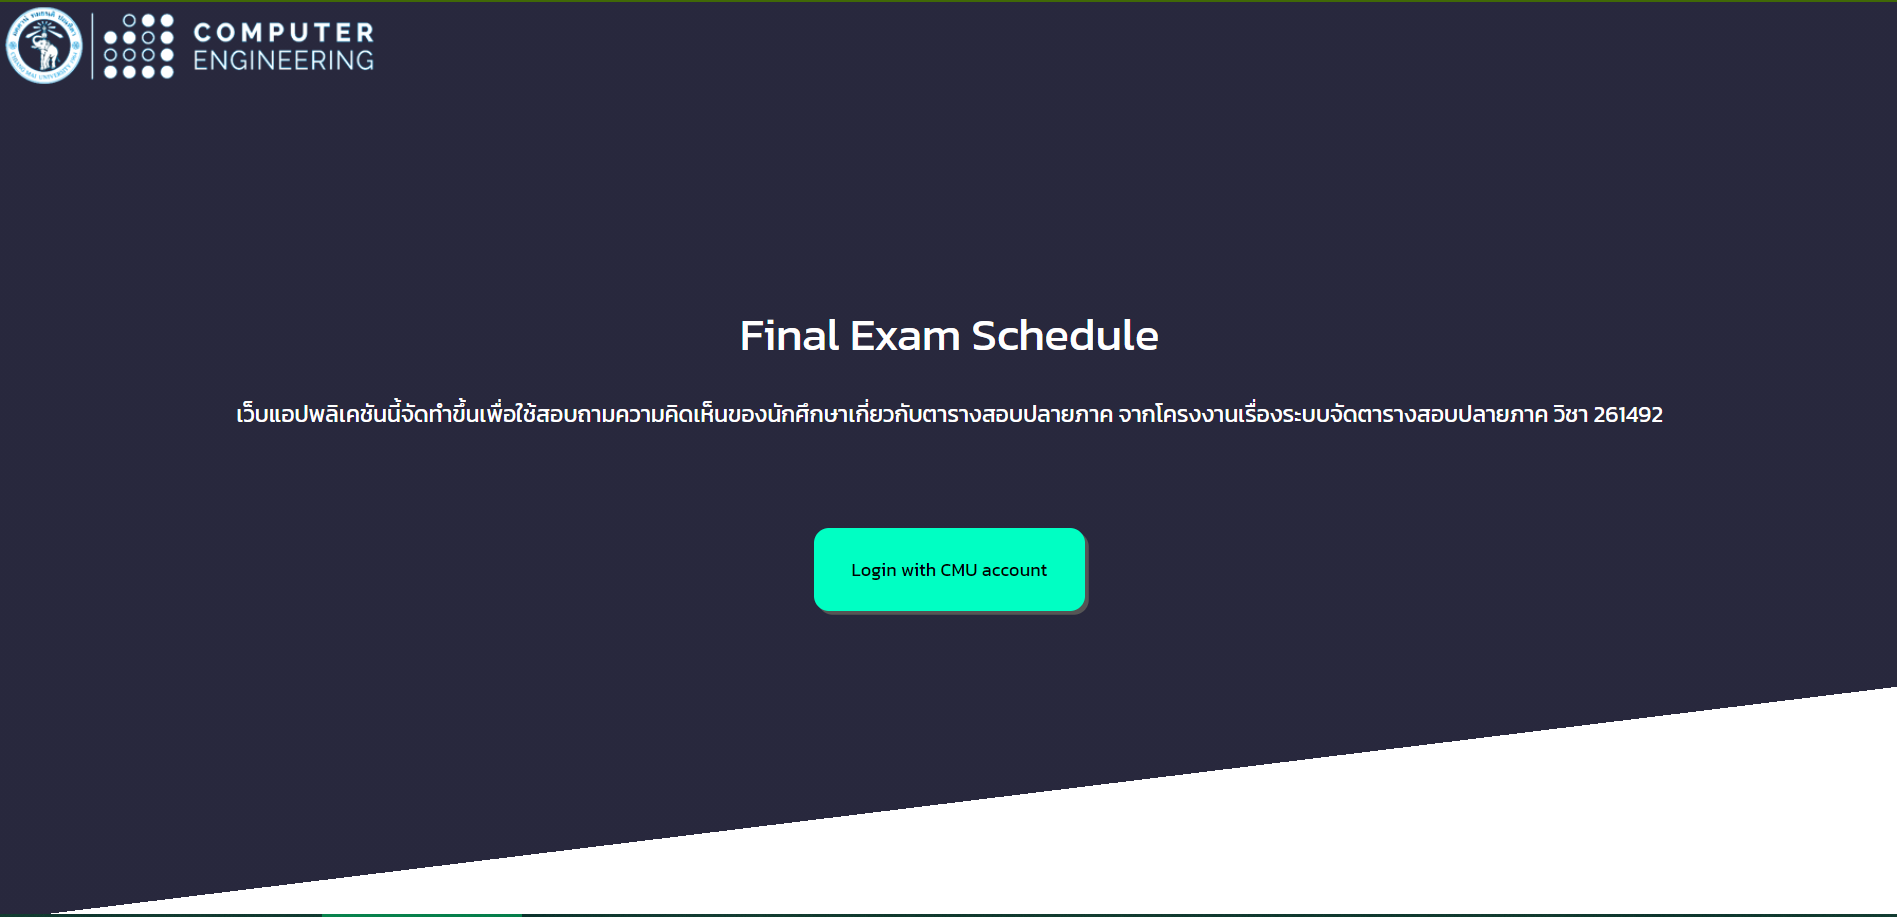
\includegraphics[width=\linewidth]{images/eval_ui_1.png}
    \end{center}
    \caption[UI หน้า Home ของเว็บแอปพลิเคชัน]{UI หน้า Home ของเว็บแอปพลิเคชัน}
    \label{fig:eval_ui_1}     
\end{figure}
\begin{figure}
    \begin{center}
      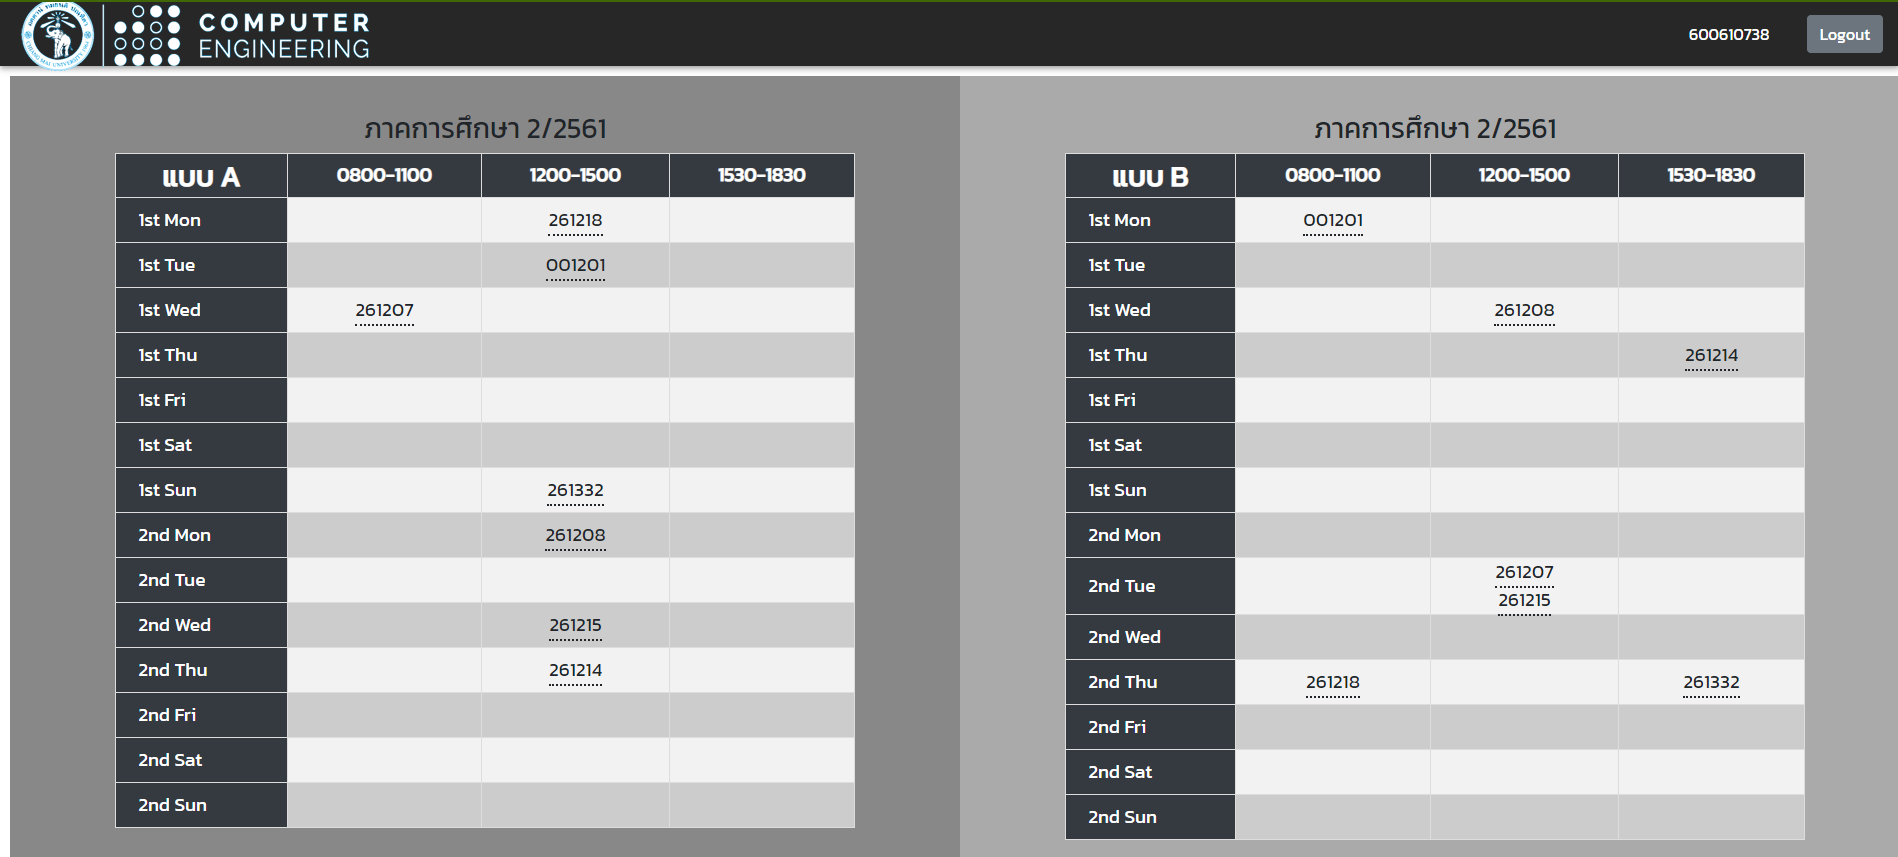
\includegraphics[width=\linewidth]{images/eval_ui_2.png}
    \end{center}
    \caption[UI หน้าแสดงตารางสอบสำหรับใช้ในการเปรียบเทียบ]{UI หน้าแสดงตารางสอบสำหรับใช้ในการเปรียบเทียบ}
    \label{fig:eval_ui_2}     
\end{figure}
\newpage
\subsection{ผลจากแบบสอบถามความพึงพอใจของนักศึกษา}
ผลการประเมินระบบโดยสอบถามความพึงพอใจของนักศึกษา ด้วยวิธีการทำ A/B Testing 
โดยให้นักศึกษาเปรียบเทียบและเลือกตารางสอบที่ตนเองชอบจากตารางสอบทั้งสองแบบโดยแบบหนึ่งเป็นตารางสอบจากสำนักทะเบียนและประมวลผล มหาวิทยาลัยเชียงใหม่ 
อีกแบบเป็นตารางสอบที่ดีที่สุดจากทุกรูปแบบที่จัดโดยโปรแกรม โดยนักศึกษาที่ทำแบบสำรวจจะไม่ทราบว่าตารางสอบที่ตนเองเห็นเป็นตารางสอบแบบใดนั้น 
ได้รับผลการตอบกลับแบบฟอร์มทั้งหมด 688 ครั้ง จากนักศึกษาจำนวน 180 คน
โดยพบว่า จากผลการสำรวจ นักศึกษามากกว่า 61\% ชอบตารางสอบที่จัดโดยโปรแกรมมากกว่าตารางสอบที่กำหนดโดยสำนักทะเบียนและประมวลผล มหาวิทยาลัยเชียงใหม่
โดยผลการนับจำนวนนักศึกษาที่เลือกระดับความพึงพอใจในตารางสอบแต่ละแบบ มีค่าเฉลี่ยความพึงพอใจเท่ากับ 0.59 และมีค่า standard deviation เท่ากับ 1.57 
โดยสามารถแจกแจงจำนวนครั้งสำหรับแต่ละระดับความพึงพอใจได้ดังรูปที่ \ref{fig:eval_result_1} และหากแจกแจงแยกตามภาคการศึกษาจะแสดงได้ดังตารางที่ \ref{tab:eval_result_2} 
\begin{figure}
    \begin{center}
      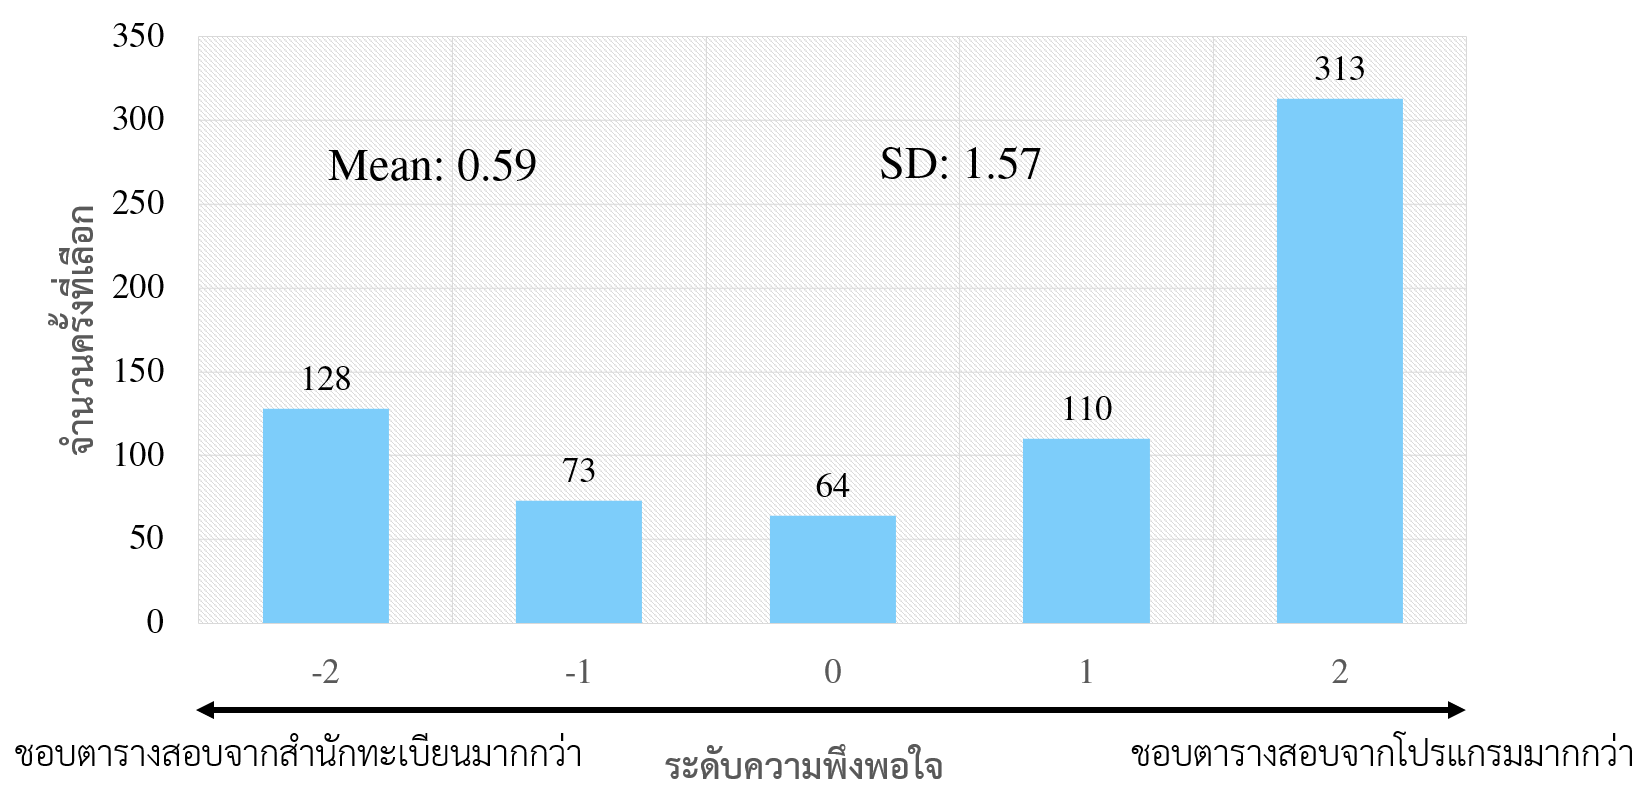
\includegraphics[width=\linewidth]{images/eval_result_1.png}
    \end{center}
    \caption[กราฟแสดงจำนวนครั้งในแต่ละระดับความพึงพอใจของนักศึกษาต่อตารางสอบ]{กราฟแสดงจำนวนครั้งในแต่ละระดับความพึงพอใจของนักศึกษาต่อตารางสอบ}
    \label{fig:eval_result_1}     
\end{figure}
\begin{table}[]
    \centering
    \resizebox{.6\textwidth}{!}{%
    \begin{tabular}{@{}cccccc@{}}
    \toprule
                               & \multicolumn{5}{c}{Total Counts of}                                                                                                         \\ \cmidrule(l){2-6} 
    \multirow{-2}{*}{Semester} & \cellcolor[HTML]{F8696B}-2 & \cellcolor[HTML]{FAB2B5}-1 & \cellcolor[HTML]{FCFCFF}0 & \cellcolor[HTML]{B0DDBD}1 & \cellcolor[HTML]{63BE7B}2 \\ \cmidrule(r){1-1}
    1/2561                     & 16                         & 15                         & 16                        & 23                        & 40                        \\
    2/2561                     & 20                         & 9                          & 5                         & 14                        & 34                        \\
    1/2562                     & 20                         & 12                         & 11                        & 10                        & 59                        \\
    2/2562                     & 15                         & 8                          & 5                         & 20                        & 65                        \\
    1/2563                     & 28                         & 15                         & 10                        & 28                        & 59                        \\
    2/2563                     & 29                         & 14                         & 17                        & 15                        & 56                        \\ \bottomrule
    \end{tabular}%
    }
    \caption{แสดงการแจกแจงจำนวนครั้งสำหรับแต่ละระดับความพึงพอใจแบ่งตามภาคการศึกษา}
    \label{tab:eval_result_2}
\end{table}

\section{การทดลองลดช่วงเวลาในการจัดสอบ}
นอกจากการทดลองจัดตารางสอบในแต่ละภาคการศึกษาที่ผ่านมา ด้วยจำนวนช่วงเวลาสอบ 42 slot หรือ 14 วัน วันละ 3 slot แล้ว
เรายังได้ทำการทดลองลดช่วงเวลาในการจัดสอบลงจาก 42 slot ให้เหลือ 36 33 และ 28 slot ตามลำดับ
เพื่อดูแนวโน้มในการเพิ่มขึ้นของ จำนวนครั้งที่มีนักศึกษาสอบสองวิชาในเวลาเดียวกันจากรูปแบบการจัดเรียงแบบต่าง ๆ เปรียบเทียบกัน
โดยได้ผลจำนวนครั้งที่มีนักศึกษาสอบสองวิชาในเวลาเดียวกันในแต่ละภาคการศึกษาและแต่ละรูปแบบการจัดเรียง ดังตารางที่ \ref{tab:overlap_count_result}
และได้ผลลัพธ์จากการคำนวนค่า penalty ของตารางสอบแต่ละภาคการศึกษา ที่จัดโดยกำหนดจำนวนช่วงเวลาในการจัดสอบต่าง ๆ กัน ดังนี้
\begin{itemize}
    \item กำหนดช่วงเวลาในการจัดสอบ 36 slot แสดงดังตารางที่ \ref{tab:result_table_161_36} -- \ref{tab:result_table_263_36}
    \item กำหนดช่วงเวลาในการจัดสอบ 33 slot แสดงดังตารางที่ \ref{tab:result_table_161_33} -- \ref{tab:result_table_263_33}
    \item กำหนดช่วงเวลาในการจัดสอบ 28 slot แสดงดังตารางที่ \ref{tab:result_table_161_28} -- \ref{tab:result_table_263_28}
\end{itemize}
ซึ่งจากผลลัพธ์จากตารางที่ \ref{tab:overlap_count_result} จะสามารถสรุปได้ว่ารูปแบบการเรียงลำดับความสำคัญในการจัดช่วงเวลาสอบให้กับวิชารูปแบบ DEG นั้น 
มีแนวโน้มที่จะจัดตารางสอบแล้วทำให้โอกาสการเกิดสถานการณ์ที่นักศึกษามีสอบสองวิชาในเวลาเดียวกันเกิดขึ้นได้น้อยที่สุด
\begin{table}[]
    \centering
    \begin{tabular}{@{}ccrrrr@{}}
    \toprule
                                  &                            & \multicolumn{4}{c}{จำนวน slot สอบ}                                                                         \\ \cmidrule(l){3-6} 
    \multirow{-2}{*}{ภาคการศึกษา} & \multirow{-2}{*}{รูปแบบ}   & 28                        & 33                       & 36                       & 42                       \\ \midrule
                                  & BFS-DEG                    & 3                         & 7                        & 3                        & 0                        \\ \cmidrule(l){2-6} 
                                  & {\color[HTML]{FE0000} DEG} & {\color[HTML]{FE0000} 0}  & {\color[HTML]{FE0000} 0} & {\color[HTML]{FE0000} 0} & {\color[HTML]{FE0000} 0} \\ \cmidrule(l){2-6} 
                                  & BFS-STD                    & 0                         & 0                        & 0                        & 0                        \\ \cmidrule(l){2-6} 
    \multirow{-4}{*}{1/2561}      & STD                        & 2                         & 0                        & 0                        & 0                        \\ \midrule
                                  & BFS-DEG                    & 24                        & 0                        & 1                        & 0                        \\ \cmidrule(l){2-6} 
                                  & {\color[HTML]{FE0000} DEG} & {\color[HTML]{FE0000} 2}  & {\color[HTML]{FE0000} 0} & {\color[HTML]{FE0000} 0} & {\color[HTML]{FE0000} 0} \\ \cmidrule(l){2-6} 
                                  & BFS-STD                    & 34                        & 8                        & 1                        & 0                        \\ \cmidrule(l){2-6} 
    \multirow{-4}{*}{2/2561}      & STD                        & 15                        & 4                        & 1                        & 0                        \\ \midrule
                                  & BFS-DEG                    & 74                        & 0                        & 5                        & 0                        \\ \cmidrule(l){2-6} 
                                  & {\color[HTML]{FE0000} DEG} & {\color[HTML]{FE0000} 2}  & {\color[HTML]{FE0000} 0} & {\color[HTML]{FE0000} 0} & {\color[HTML]{FE0000} 0} \\ \cmidrule(l){2-6} 
                                  & BFS-STD                    & 14                        & 0                        & 0                        & 0                        \\ \cmidrule(l){2-6} 
    \multirow{-4}{*}{1/2562}      & STD                        & 26                        & 5                        & 0                        & 0                        \\ \midrule
                                  & BFS-DEG                    & 286                       & 149                      & 42                       & 0                        \\ \cmidrule(l){2-6} 
                                  & {\color[HTML]{FE0000} DEG} & {\color[HTML]{FE0000} 6}  & {\color[HTML]{FE0000} 0} & {\color[HTML]{FE0000} 0} & {\color[HTML]{FE0000} 0} \\ \cmidrule(l){2-6} 
                                  & BFS-STD                    & 34                        & 1                        & 4                        & 0                        \\ \cmidrule(l){2-6} 
    \multirow{-4}{*}{2/2562}      & STD                        & 54                        & 7                        & 5                        & 0                        \\ \midrule
                                  & BFS-DEG                    & 25                        & 1                        & 0                        & 0                        \\ \cmidrule(l){2-6} 
                                  & {\color[HTML]{FE0000} DEG} & {\color[HTML]{FE0000} 25} & {\color[HTML]{FE0000} 1} & {\color[HTML]{FE0000} 0} & {\color[HTML]{FE0000} 0} \\ \cmidrule(l){2-6} 
                                  & BFS-STD                    & 65                        & 12                       & 2                        & 0                        \\ \cmidrule(l){2-6} 
    \multirow{-4}{*}{1/2563}      & STD                        & 50                        & 16                       & 8                        & 0                        \\ \midrule
                                  & BFS-DEG                    & 56                        & 19                       & 0                        & 0                        \\ \cmidrule(l){2-6} 
                                  & {\color[HTML]{FE0000} DEG} & {\color[HTML]{FE0000} 17} & {\color[HTML]{FE0000} 1} & {\color[HTML]{FE0000} 0} & {\color[HTML]{FE0000} 0} \\ \cmidrule(l){2-6} 
                                  & BFS-STD                    & 66                        & 9                        & 2                        & 0                        \\ \cmidrule(l){2-6} 
    \multirow{-4}{*}{2/2563}      & STD                        & 47                        & 10                       & 2                        & 1                        \\ \bottomrule
    \end{tabular}
    \caption{ตารางแสดงจำนวนครั้งที่มีนักศึกษาสอบสองวิชาในเวลาเดียวกัน}
    \label{tab:overlap_count_result}
    \end{table}
\begin{table}[]
    \centering
    \textbf{Total courses: 1432} \quad \quad \textbf{Total students having an exam: 13171}
    \resizebox{\textwidth}{!}{%
    \begin{tabular}{@{}ccrrrrrrrr@{}}
    \toprule
    \textbf{รูปแบบ}                              & \textbf{Penalty}                      & \textbf{1}                  & \textbf{2}                    & \textbf{3}                    & \textbf{4}                    & \textbf{5}                    & \textbf{6}                   & \textbf{7}                    & \textbf{รวม}                  \\ \midrule
                                                & \textbf{Count}                        & 0                              & 3                              & 822                            & 1009                           & 1090                           & 553                            & 6578                           & 10055                            \\ \cmidrule(l){2-10} 
    \multirow{-2}{*}{BFS-DEG}                   & \textbf{Value}                        & 0                              & 30000                          & 64116                          & 78702                          & 41420                          & 16037                          & 78936                          & 309211                           \\ \midrule
                                                & \textbf{Count}                        & 0                              &  0                             &  997                           &  202                           & 548                            &  136                           &  8029                          & 9912      \\ \cmidrule(l){2-10} 
    \multirow{-2}{*}{DEG}                       & \textbf{Value}                        & 0                              &  0                             &  77766                         &  15756                         & 20824                          &  3944                          & 96348                          & 214638    \\ \midrule
                                                 & \textbf{Count}                        & 1                              & 0                              & 1473                           & 353                            & 319                            & 202                            & 6423                           & 8771                             \\ \cmidrule(l){2-10} 
    \multirow{-2}{*}{BFS-STD}                    & \textbf{Value}                        & 2                              & 0                              & 114894                         & 27534                          & 12122                          & 5858                           & 77076                          & 237486                           \\ \midrule
    {\color[HTML]{FE0000} }                      & {\color[HTML]{FE0000} \textbf{Count}} & {\color[HTML]{FE0000} 0}       & {\color[HTML]{FE0000} 0}       & {\color[HTML]{FE0000} 808}     & {\color[HTML]{FE0000} 348}     & {\color[HTML]{FE0000} 349}     & {\color[HTML]{FE0000} 180}     & {\color[HTML]{FE0000} 6988}    & {\color[HTML]{FE0000} 8673}      \\ \cmidrule(l){2-10} 
    \multirow{-2}{*}{{\color[HTML]{FE0000} STD}} & {\color[HTML]{FE0000} \textbf{Value}} & {\color[HTML]{FE0000} 0}       & {\color[HTML]{FE0000} 0}       & {\color[HTML]{FE0000} 63024}   & {\color[HTML]{FE0000} 27144}   & {\color[HTML]{FE0000} 13262}   & {\color[HTML]{FE0000} 5220}    & {\color[HTML]{FE0000} 83856}   & {\color[HTML]{FE0000} 192506}    \\ \bottomrule
    \end{tabular}%
    }
    \caption{ตารางแสดงค่า penalty ของตารางสอบเทอม 1/2561 ที่จัดสอบ 36 slot}
    \label{tab:result_table_161_36}
\end{table}
\begin{table}[]
    \centering
    \textbf{Total courses: 1551} \quad \quad \textbf{Total students having an exam: 13095}
    \resizebox{\textwidth}{!}{%
    \begin{tabular}{@{}ccrrrrrrrr@{}}
    \toprule
    \textbf{รูปแบบ}                              & \textbf{Penalty}                      & \textbf{1}                  & \textbf{2}                    & \textbf{3}                    & \textbf{4}                    & \textbf{5}                    & \textbf{6}                   & \textbf{7}                    & \textbf{รวม}                  \\ \midrule
                                                 & \textbf{Count}                        & 1                              & 1                              & 2510                           & 1165                           & 979                            & 1063                           & 7736                           & 13455                            \\ \cmidrule(l){2-10} 
    \multirow{-2}{*}{BFS-DEG}                    & \textbf{Value}                        & 2                              & 10000                          & 195780                         & 90870                          & 37202                          & 30827                          & 92832                          & 457513                           \\ \midrule
    {\color[HTML]{FE0000} }                      & {\color[HTML]{FE0000} \textbf{Count}} & {\color[HTML]{FE0000} 1}       & {\color[HTML]{FE0000} 0}       & {\color[HTML]{FE0000} 1823}    & {\color[HTML]{FE0000} 708}     & {\color[HTML]{FE0000} 554}     & {\color[HTML]{FE0000} 555}     & {\color[HTML]{FE0000} 7449}    & {\color[HTML]{FE0000} 11090}     \\ \cmidrule(l){2-10} 
    \multirow{-2}{*}{{\color[HTML]{FE0000} DEG}} & {\color[HTML]{FE0000} \textbf{Value}} & {\color[HTML]{FE0000} 1103}    & {\color[HTML]{FE0000} 0}       & {\color[HTML]{FE0000} 142194}  & {\color[HTML]{FE0000} 55224}   & {\color[HTML]{FE0000} 21052}   & {\color[HTML]{FE0000} 16095}   & {\color[HTML]{FE0000} 89388}   & {\color[HTML]{FE0000} 325056}    \\ \midrule
                                                 & \textbf{Count}                        & 1                              & 1                              & 2240                           & 862                            & 745                            & 422                            & 6407                           & 10678                            \\ \cmidrule(l){2-10} 
    \multirow{-2}{*}{BFS-STD}                    & \textbf{Value}                        & 2                              & 10000                          & 174720                         & 67236                          & 28310                          & 12238                          & 76884                          & 369390                           \\ \midrule
                                                  & {\textbf{Count}} & {0}       & {1}       & {1585}    & {821}     & {619}     & {451}     & {5957}    & {9434}      \\ \cmidrule(l){2-10} 
    \multirow{-2}{*}{STD} & {\textbf{Value}} & {0}       & {10000}   & {123630}  & {64038}   & {23522}   & {13079}   & {71484}   & {305753}    \\ \bottomrule
    \end{tabular}%
    }
    \caption{ตารางแสดงค่า penalty ของตารางสอบเทอม 2/2561 ที่จัดสอบ 36 slot}
    \label{tab:result_table_261_36}
\end{table}
\begin{table}[]
    \centering
    \textbf{Total courses: 1729} \quad \quad \textbf{Total students having an exam: 19786}
    \resizebox{\textwidth}{!}{%
    \begin{tabular}{@{}ccrrrrrrrr@{}}
    \toprule
    \textbf{รูปแบบ}                              & \textbf{Penalty}                      & \textbf{1}                  & \textbf{2}                    & \textbf{3}                    & \textbf{4}                    & \textbf{5}                    & \textbf{6}                   & \textbf{7}                    & \textbf{รวม}                  \\ \midrule
                                                 & \textbf{Count}                        & 2                              & 5                              & 3393                           & 779                            & 798                            & 996                            & 11979                          & 17952                            \\ \cmidrule(l){2-10} 
    \multirow{-2}{*}{BFS-DEG}                    & \textbf{Value}                        & 17690                          & 50000                          & 264654                         & 60762                          & 30324                          & 28884                          & 143748                         & 596062                           \\ \midrule
                                                  & {\textbf{Count}} & {2}       & {0}       & {2817}    & {545}     & {979}     & {364}     & {10000}   & {14707}     \\ \cmidrule(l){2-10} 
    \multirow{-2}{*}{DEG} & {\textbf{Value}} & {7829}    & {0}       & {219726}  & {42510}   & {37202}   & {10556}   & {120000}  & {437823}    \\ \midrule
                                                 & \textbf{Count}                        & 1                              & 0                              & 2618                           & 1043                           & 534                            & 477                            & 10681                          & 15354                            \\ \cmidrule(l){2-10} 
    \multirow{-2}{*}{BFS-STD}                    & \textbf{Value}                        & 2                              & 0                              & 204204                         & 81354                          & 20292                          & 13833                          & 128172                         & 447857                           \\ \midrule
    {\color[HTML]{FE0000} }                      & {\color[HTML]{FE0000} \textbf{Count}} & {\color[HTML]{FE0000} 2}       & {\color[HTML]{FE0000} 0}       & {\color[HTML]{FE0000} 1557}    & {\color[HTML]{FE0000} 896}     & {\color[HTML]{FE0000} 819}     & {\color[HTML]{FE0000} 401}     & {\color[HTML]{FE0000} 10745}   & {\color[HTML]{FE0000} 14420}     \\ \cmidrule(l){2-10} 
    \multirow{-2}{*}{{\color[HTML]{FE0000} STD}} & {\color[HTML]{FE0000} \textbf{Value}} & {\color[HTML]{FE0000} 1399}    & {\color[HTML]{FE0000} 0}       & {\color[HTML]{FE0000} 121446}  & {\color[HTML]{FE0000} 69888}   & {\color[HTML]{FE0000} 31122}   & {\color[HTML]{FE0000} 11629}   & {\color[HTML]{FE0000} 128940}  & {\color[HTML]{FE0000} 364424}    \\ \bottomrule
    \end{tabular}%
    }
    \caption{ตารางแสดงค่า penalty ของตารางสอบเทอม 1/2562 ที่จัดสอบ 36 slot}
    \label{tab:result_table_162_36}
\end{table}
\begin{table}[]
    \centering
    \textbf{Total courses: 1828} \quad \quad \textbf{Total students having an exam: 19505}
    \resizebox{\textwidth}{!}{%
    \begin{tabular}{@{}ccrrrrrrrr@{}}
    \toprule
    \textbf{รูปแบบ}                              & \textbf{Penalty}                      & \textbf{1}                  & \textbf{2}                    & \textbf{3}                    & \textbf{4}                    & \textbf{5}                    & \textbf{6}                   & \textbf{7}                    & \textbf{รวม}                  \\ \midrule
                                                 & \textbf{Count}                        & 1                              & 42                             & 2584                           & 1856                           & 1796                           & 1924                           & 10106                          & 18309                            \\ \cmidrule(l){2-10} 
    \multirow{-2}{*}{BFS-DEG}                    & \textbf{Value}                        & 2445                           & 420000                         & 201552                         & 144768                         & 68248                          & 55796                          & 121272                         & 1014081                          \\ \midrule
    {\color[HTML]{FE0000} }                      & {\color[HTML]{FE0000} \textbf{Count}} & {\color[HTML]{FE0000} 2}       & {\color[HTML]{FE0000} 0}       & {\color[HTML]{FE0000} 2810}    & {\color[HTML]{FE0000} 814}     & {\color[HTML]{FE0000} 953}     & {\color[HTML]{FE0000} 648}     & {\color[HTML]{FE0000} 11006}   & {\color[HTML]{FE0000} 16233}     \\ \cmidrule(l){2-10} 
    \multirow{-2}{*}{{\color[HTML]{FE0000} DEG}} & {\color[HTML]{FE0000} \textbf{Value}} & {\color[HTML]{FE0000} 3110}    & {\color[HTML]{FE0000} 0}       & {\color[HTML]{FE0000} 219180}  & {\color[HTML]{FE0000} 63492}   & {\color[HTML]{FE0000} 36214}   & {\color[HTML]{FE0000} 18792}   & {\color[HTML]{FE0000} 132072}  & {\color[HTML]{FE0000} 472860}    \\ \midrule
                                                 & \textbf{Count}                        & 1                              & 4                              & 3682                           & 1447                           & 717                            & 595                            & 9760                           & 16206                            \\ \cmidrule(l){2-10} 
    \multirow{-2}{*}{BFS-STD}                    & \textbf{Value}                        & 1011393                        & 40000                          & 287196                         & 112866                         & 27246                          & 17255                          & 117120                         & 1613076                          \\ \midrule
                                                  & {\textbf{Count}} & {1}       & {5}       & {2850}    & {969}     & {731}     & {523}     & {9420}    & {14499}     \\ \cmidrule(l){2-10} 
    \multirow{-2}{*}{STD} & {\textbf{Value}} & {649}     & {50000}   & {222300}  & {75582}   & {27778}   & {15167}   & {113040}  & {504516}    \\ \bottomrule
    \end{tabular}%
    }
    \caption{ตารางแสดงค่า penalty ของตารางสอบเทอม 2/2562 ที่จัดสอบ 36 slot}
    \label{tab:result_table_262_36}
\end{table}
\begin{table}[]
    \centering
    \textbf{Total courses: 1894} \quad \quad \textbf{Total students having an exam: 26549}
    \resizebox{\textwidth}{!}{%
    \begin{tabular}{@{}ccrrrrrrrr@{}}
    \toprule
    \textbf{รูปแบบ}                              & \textbf{Penalty}                      & \textbf{1}                  & \textbf{2}                    & \textbf{3}                    & \textbf{4}                    & \textbf{5}                    & \textbf{6}                   & \textbf{7}                    & \textbf{รวม}                  \\ \midrule
                                                 & \textbf{Count}                        & 2                              & 0                              & 3931                           & 1772                           & 1828                           & 1831                           & 15541                          & 24905                            \\ \cmidrule(l){2-10} 
    \multirow{-2}{*}{BFS-DEG}                    & \textbf{Value}                        & 24759                          & 0                              & 306618                         & 138216                         & 69464                          & 53099                          & 186492                         & 778648                           \\ \midrule
    {\color[HTML]{FE0000} }                      & {\color[HTML]{FE0000} \textbf{Count}} & {\color[HTML]{FE0000} 1}       & {\color[HTML]{FE0000} 0}       & {\color[HTML]{FE0000} 4224}    & {\color[HTML]{FE0000} 1646}    & {\color[HTML]{FE0000} 1444}    & {\color[HTML]{FE0000} 1817}    & {\color[HTML]{FE0000} 15491}   & {\color[HTML]{FE0000} 24623}     \\ \cmidrule(l){2-10} 
    \multirow{-2}{*}{{\color[HTML]{FE0000} DEG}} & {\color[HTML]{FE0000} \textbf{Value}} & {\color[HTML]{FE0000} 18726}   & {\color[HTML]{FE0000} 0}       & {\color[HTML]{FE0000} 329472}  & {\color[HTML]{FE0000} 128388}  & {\color[HTML]{FE0000} 54872}   & {\color[HTML]{FE0000} 52693}   & {\color[HTML]{FE0000} 185892}  & {\color[HTML]{FE0000} 770043}    \\ \midrule
                                                 & \textbf{Count}                        & 3                              & 2                              & 3204                           & 1342                           & 953                            & 843                            & 13295                          & 19642                            \\ \cmidrule(l){2-10} 
    \multirow{-2}{*}{BFS-STD}                    & \textbf{Value}                        & 25398                          & 20000                          & 249912                         & 104676                         & 36214                          & 24447                          & 159540                         & 620187                           \\ \midrule
                                                  & {\textbf{Count}} & {2}       & {8}       & {3254}    & {1965}    & {1032}    & {854}     & {15233}   & {22348}     \\ \cmidrule(l){2-10} 
    \multirow{-2}{*}{STD} & {\textbf{Value}} & {8152}    & {80000}   & {253812}  & {153270}  & {39216}   & {24766}   & {182796}  & {742012}    \\ \bottomrule
    \end{tabular}%
    }
    \caption{ตารางแสดงค่า penalty ของตารางสอบเทอม 1/2563 ที่จัดสอบ 36 slot}
    \label{tab:result_table_163_36}
\end{table}
\begin{table}[]
    \centering
    \textbf{Total courses: 1770} \quad \quad \textbf{Total students having an exam: 24392}
    \resizebox{\textwidth}{!}{%
    \begin{tabular}{@{}ccrrrrrrrr@{}}
    \toprule
    \textbf{รูปแบบ}                              & \textbf{Penalty}                      & \textbf{1}                  & \textbf{2}                    & \textbf{3}                    & \textbf{4}                    & \textbf{5}                    & \textbf{6}                   & \textbf{7}                    & \textbf{รวม}                  \\ \midrule
                                                 & \textbf{Count}                        & 1                              & 0                              & 4051                           & 1706                           & 1747                           & 1434                           & 17147                          & 26086                            \\ \cmidrule(l){2-10} 
    \multirow{-2}{*}{BFS-DEG}                    & \textbf{Value}                        & 4                              & 0                              & 315978                         & 133068                         & 66386                          & 41586                          & 205764                         & 762786                           \\ \midrule
    {\color[HTML]{FE0000} }                      & {\color[HTML]{FE0000} \textbf{Count}} & {\color[HTML]{FE0000} 2}       & {\color[HTML]{FE0000} 0}       & {\color[HTML]{FE0000} 3449}    & {\color[HTML]{FE0000} 1624}    & {\color[HTML]{FE0000} 1454}    & {\color[HTML]{FE0000} 913}     & {\color[HTML]{FE0000} 15549}   & {\color[HTML]{FE0000} 22991}     \\ \cmidrule(l){2-10} 
    \multirow{-2}{*}{{\color[HTML]{FE0000} DEG}} & {\color[HTML]{FE0000} \textbf{Value}} & {\color[HTML]{FE0000} 758}     & {\color[HTML]{FE0000} 0}       & {\color[HTML]{FE0000} 269022}  & {\color[HTML]{FE0000} 126672}  & {\color[HTML]{FE0000} 55252}   & {\color[HTML]{FE0000} 26477}   & {\color[HTML]{FE0000} 186588}  & {\color[HTML]{FE0000} 664769}    \\ \midrule
                                                 & \textbf{Count}                        & 1                              & 2                              & 4113                           & 2617                           & 981                            & 1018                           & 16764                          & 25496                            \\ \cmidrule(l){2-10} 
    \multirow{-2}{*}{BFS-STD}                    & \textbf{Value}                        & 674                            & 20000                          & 320814                         & 204126                         & 37278                          & 29522                          & 201168                         & 813582                           \\ \midrule
                                                  & {\textbf{Count}} & {2}       & {2}       & {3235}    & {1543}    & {883}     & {707}     & {14640}   & {21012}     \\ \cmidrule(l){2-10} 
    \multirow{-2}{*}{STD} & {\textbf{Value}} & {1038}    & {20000}   & {252330}  & {120354}  & {33554}   & {20503}   & {175680}  & {623459}    \\ \bottomrule
    \end{tabular}%
    }
    \caption{ตารางแสดงค่า penalty ของตารางสอบเทอม 2/2563 ที่จัดสอบ 36 slot}
    \label{tab:result_table_263_36}
\end{table}
\begin{table}[]
    \centering
    \textbf{Total courses: 1432} \quad \quad \textbf{Total students having an exam: 13171}
    \resizebox{\textwidth}{!}{%
    \begin{tabular}{@{}ccrrrrrrrr@{}}
    \toprule
    \textbf{รูปแบบ}                              & \textbf{Penalty}                      & \textbf{1}                  & \textbf{2}                    & \textbf{3}                    & \textbf{4}                    & \textbf{5}                    & \textbf{6}                   & \textbf{7}                    & \textbf{รวม}                  \\ \midrule
                                                 & \textbf{Count}                        & 0                              & 7                              & 1567                           & 1151                           & 1387                           & 594                            & 4660                           & 9366                             \\ \cmidrule(l){2-10} 
    \multirow{-2}{*}{BFS-DEG}                    & \textbf{Value}                        & 0                              & 70000                          & 122226                         & 89778                          & 52706                          & 17226                          & 55920                          & 407856                           \\ \midrule
                                                  & {\textbf{Count}} & {2}       & {0}       & {1486}    & {392}     & {739}     & {544}     & {4610}    & {7773}      \\ \cmidrule(l){2-10} 
    \multirow{-2}{*}{DEG} & {\textbf{Value}} & {1363}    & {0}       & {115908}  & {30576}   & {28082}   & {15776}   & {55320}   & {247025}    \\ \midrule
                                                 & \textbf{Count}                        & 1                              & 0                              & 1900                           & 797                            & 499                            & 269                            & 5023                           & 8489                             \\ \cmidrule(l){2-10} 
    \multirow{-2}{*}{BFS-STD}                    & \textbf{Value}                        & 2                              & 0                              & 148200                         & 62166                          & 18962                          & 7801                           & 60276                          & 297407                           \\ \midrule
    {\color[HTML]{FE0000} }                      & {\color[HTML]{FE0000} \textbf{Count}} & {\color[HTML]{FE0000} 1}       & {\color[HTML]{FE0000} 0}       & {\color[HTML]{FE0000} 1267}    & {\color[HTML]{FE0000} 462}     & {\color[HTML]{FE0000} 527}     & {\color[HTML]{FE0000} 274}     & {\color[HTML]{FE0000} 4580}    & {\color[HTML]{FE0000} 7111}      \\ \cmidrule(l){2-10} 
    \multirow{-2}{*}{{\color[HTML]{FE0000} STD}} & {\color[HTML]{FE0000} \textbf{Value}} & {\color[HTML]{FE0000} 541}     & {\color[HTML]{FE0000} 0}       & {\color[HTML]{FE0000} 98826}   & {\color[HTML]{FE0000} 36036}   & {\color[HTML]{FE0000} 20026}   & {\color[HTML]{FE0000} 7946}    & {\color[HTML]{FE0000} 54960}   & {\color[HTML]{FE0000} 218335}    \\ \bottomrule
    \end{tabular}%
    }
    \caption{ตารางแสดงค่า penalty ของตารางสอบเทอม 1/2561 ที่จัดสอบ 33 slot}
    \label{tab:result_table_161_33}
\end{table}
\begin{table}[]
    \centering
    \textbf{Total courses: 1551} \quad \quad \textbf{Total students having an exam: 13095}
    \resizebox{\textwidth}{!}{%
    \begin{tabular}{@{}ccrrrrrrrr@{}}
    \toprule
    \textbf{รูปแบบ}                              & \textbf{Penalty}                      & \textbf{1}                  & \textbf{2}                    & \textbf{3}                    & \textbf{4}                    & \textbf{5}                    & \textbf{6}                   & \textbf{7}                    & \textbf{รวม}                  \\ \midrule
                                                 & \textbf{Count}                        & 1                              & 0                              & 3361                           & 1223                           & 2317                           & 1175                           & 5159                           & 13236                            \\ \cmidrule(l){2-10} 
    \multirow{-2}{*}{BFS-DEG}                    & \textbf{Value}                        & 2                              & 0                              & 262158                         & 95394                          & 88046                          & 34075                          & 61908                          & 541583                           \\ \midrule
    {\color[HTML]{FE0000} }                      & {\color[HTML]{FE0000} \textbf{Count}} & {\color[HTML]{FE0000} 0}       & {\color[HTML]{FE0000} 0}       & {\color[HTML]{FE0000} 2875}    & {\color[HTML]{FE0000} 1319}    & {\color[HTML]{FE0000} 1546}    & {\color[HTML]{FE0000} 774}     & {\color[HTML]{FE0000} 5120}    & {\color[HTML]{FE0000} 11634}     \\ \cmidrule(l){2-10} 
    \multirow{-2}{*}{{\color[HTML]{FE0000} DEG}} & {\color[HTML]{FE0000} \textbf{Value}} & {\color[HTML]{FE0000} 0}       & {\color[HTML]{FE0000} 0}       & {\color[HTML]{FE0000} 224250}  & {\color[HTML]{FE0000} 102882}  & {\color[HTML]{FE0000} 58748}   & {\color[HTML]{FE0000} 22446}   & {\color[HTML]{FE0000} 61440}   & {\color[HTML]{FE0000} 469766}    \\ \midrule
                                                 & \textbf{Count}                        & 1                              & 8                              & 2837                           & 1705                           & 862                            & 969                            & 5560                           & 11942                            \\ \cmidrule(l){2-10} 
    \multirow{-2}{*}{BFS-STD}                    & \textbf{Value}                        & 11808635                       & 80000                          & 221286                         & 132990                         & 32756                          & 28101                          & 66720                          & 12370488                         \\ \midrule
                                                  & {\textbf{Count}} & {1}       & {4}       & {2562}    & {1096}    & {828}     & {520}     & {5109}    & {10120}     \\ \cmidrule(l){2-10} 
    \multirow{-2}{*}{STD} & {\textbf{Value}} & {2467}    & {40000}   & {199836}  & {85488}   & {31464}   & {15080}   & {61308}   & {435643}    \\ \bottomrule
    \end{tabular}%
    }
    \caption{ตารางแสดงค่า penalty ของตารางสอบเทอม 2/2561 ที่จัดสอบ 33 slot}
    \label{tab:result_table_261_33}
\end{table}
\begin{table}[]
    \centering
    \textbf{Total courses: 1729} \quad \quad \textbf{Total students having an exam: 19786}
    \resizebox{\textwidth}{!}{%
    \begin{tabular}{@{}ccrrrrrrrr@{}}
    \toprule
    \textbf{รูปแบบ}                              & \textbf{Penalty}                      & \textbf{1}                  & \textbf{2}                    & \textbf{3}                    & \textbf{4}                    & \textbf{5}                    & \textbf{6}                   & \textbf{7}                    & \textbf{รวม}                  \\ \midrule
                                                 & \textbf{Count}                        & 0                              & 0                              & 3707                           & 1286                           & 3717                           & 1911                           & 9393                           & 20014                            \\ \cmidrule(l){2-10} 
    \multirow{-2}{*}{BFS-DEG}                    & \textbf{Value}                        & 0                              & 0                              & 289146                         & 100308                         & 141246                         & 55419                          & 112716                         & 698835                           \\ \midrule
    {\color[HTML]{FE0000} }                      & {\color[HTML]{FE0000} \textbf{Count}} & {\color[HTML]{FE0000} 1}       & {\color[HTML]{FE0000} 0}       & {\color[HTML]{FE0000} 3423}    & {\color[HTML]{FE0000} 805}     & {\color[HTML]{FE0000} 1168}    & {\color[HTML]{FE0000} 719}     & {\color[HTML]{FE0000} 7017}    & {\color[HTML]{FE0000} 13133}     \\ \cmidrule(l){2-10} 
    \multirow{-2}{*}{{\color[HTML]{FE0000} DEG}} & {\color[HTML]{FE0000} \textbf{Value}} & {\color[HTML]{FE0000} 15169}   & {\color[HTML]{FE0000} 0}       & {\color[HTML]{FE0000} 266994}  & {\color[HTML]{FE0000} 62790}   & {\color[HTML]{FE0000} 44384}   & {\color[HTML]{FE0000} 20851}   & {\color[HTML]{FE0000} 84204}   & {\color[HTML]{FE0000} 494392}    \\ \midrule
                                                 & \textbf{Count}                        & 1                              & 0                              & 3261                           & 1275                           & 853                            & 604                            & 8338                           & 14332                            \\ \cmidrule(l){2-10} 
    \multirow{-2}{*}{BFS-STD}                    & \textbf{Value}                        & 2                              & 0                              & 254358                         & 99450                          & 32414                          & 17516                          & 100056                         & 503796                           \\ \midrule
                                                  & {\textbf{Count}} & {2}       & {5}       & {2752}    & {1270}    & {1130}    & {821}     & {10692}   & {16672}     \\ \cmidrule(l){2-10} 
    \multirow{-2}{*}{STD} & {\textbf{Value}} & {3589}    & {50000}   & {214656}  & {99060}   & {42940}   & {23809}   & {128304}  & {562358}    \\ \bottomrule
    \end{tabular}%
    }
    \caption{ตารางแสดงค่า penalty ของตารางสอบเทอม 1/2562 ที่จัดสอบ 33 slot}
    \label{tab:result_table_162_33}
\end{table}
\begin{table}[]
    \centering
    \textbf{Total courses: 1828} \quad \quad \textbf{Total students having an exam: 19505}
    \resizebox{\textwidth}{!}{%
    \begin{tabular}{@{}ccrrrrrrrr@{}}
    \toprule
    \textbf{รูปแบบ}                              & \textbf{Penalty}                      & \textbf{1}                  & \textbf{2}                    & \textbf{3}                    & \textbf{4}                    & \textbf{5}                    & \textbf{6}                   & \textbf{7}                    & \textbf{รวม}                  \\ \midrule
                                                 & \textbf{Count}                        & 1                              & 149                            & 4350                           & 2334                           & 2942                           & 2136                           & 8759                           & 20671                            \\ \cmidrule(l){2-10} 
    \multirow{-2}{*}{BFS-DEG}                    & \textbf{Value}                        & 5064                           & 1490000                        & 339300                         & 182052                         & 111796                         & 61944                          & 105108                         & 2295264                          \\ \midrule
    {\color[HTML]{FE0000} }                      & {\color[HTML]{FE0000} \textbf{Count}} & {\color[HTML]{FE0000} 1}       & {\color[HTML]{FE0000} 0}       & {\color[HTML]{FE0000} 4603}    & {\color[HTML]{FE0000} 1680}    & {\color[HTML]{FE0000} 1593}    & {\color[HTML]{FE0000} 1057}    & {\color[HTML]{FE0000} 9107}    & {\color[HTML]{FE0000} 18041}     \\ \cmidrule(l){2-10} 
    \multirow{-2}{*}{{\color[HTML]{FE0000} DEG}} & {\color[HTML]{FE0000} \textbf{Value}} & {\color[HTML]{FE0000} 6143}    & {\color[HTML]{FE0000} 0}       & {\color[HTML]{FE0000} 359034}  & {\color[HTML]{FE0000} 131040}  & {\color[HTML]{FE0000} 60534}   & {\color[HTML]{FE0000} 30653}   & {\color[HTML]{FE0000} 109284}  & {\color[HTML]{FE0000} 696688}    \\ \midrule
                                                 & \textbf{Count}                        & 1                              & 1                              & 3510                           & 1802                           & 1093                           & 904                            & 7822                           & 15133                            \\ \cmidrule(l){2-10} 
    \multirow{-2}{*}{BFS-STD}                    & \textbf{Value}                        & 1321733                        & 10000                          & 273780                         & 140556                         & 41534                          & 26216                          & 93864                          & 1907683                          \\ \midrule
                                                  & {\textbf{Count}} & {1}       & {7}       & {3529}    & {1747}    & {751}     & {788}     & {7574}    & {14397}     \\ \cmidrule(l){2-10} 
    \multirow{-2}{*}{STD} & {\textbf{Value}} & {16411}   & {70000}   & {275262}  & {136266}  & {28538}   & {22852}   & {90888}   & {640217}    \\ \bottomrule
    \end{tabular}%
    }
    \caption{ตารางแสดงค่า penalty ของตารางสอบเทอม 2/2562 ที่จัดสอบ 33 slot}
    \label{tab:result_table_262_33}
\end{table}
\begin{table}[]
    \centering
    \textbf{Total courses: 1894} \quad \quad \textbf{Total students having an exam: 26549}
    \resizebox{\textwidth}{!}{%
    \begin{tabular}{@{}ccrrrrrrrr@{}}
    \toprule
    \textbf{รูปแบบ}                              & \textbf{Penalty}                      & \textbf{1}                  & \textbf{2}                    & \textbf{3}                    & \textbf{4}                    & \textbf{5}                    & \textbf{6}                   & \textbf{7}                    & \textbf{รวม}                  \\ \midrule
                                                 & \textbf{Count}                        & 2                              & 1                              & 4542                           & 2696                           & 2132                           & 1951                           & 11536                          & 22860                            \\ \cmidrule(l){2-10} 
    \multirow{-2}{*}{BFS-DEG}                    & \textbf{Value}                        & 39656                          & 10000                          & 354276                         & 210288                         & 81016                          & 56579                          & 138432                         & 890247                           \\ \midrule
    {\color[HTML]{FE0000} }                      & {\color[HTML]{FE0000} \textbf{Count}} & {\color[HTML]{FE0000} 1}       & {\color[HTML]{FE0000} 1}       & {\color[HTML]{FE0000} 4676}    & {\color[HTML]{FE0000} 2917}    & {\color[HTML]{FE0000} 1984}    & {\color[HTML]{FE0000} 1903}    & {\color[HTML]{FE0000} 10809}   & {\color[HTML]{FE0000} 22291}     \\ \cmidrule(l){2-10} 
    \multirow{-2}{*}{{\color[HTML]{FE0000} DEG}} & {\color[HTML]{FE0000} \textbf{Value}} & {\color[HTML]{FE0000} 21235}   & {\color[HTML]{FE0000} 10000}   & {\color[HTML]{FE0000} 364728}  & {\color[HTML]{FE0000} 227526}  & {\color[HTML]{FE0000} 75392}   & {\color[HTML]{FE0000} 55187}   & {\color[HTML]{FE0000} 129708}  & {\color[HTML]{FE0000} 883776}    \\ \midrule
                                                 & \textbf{Count}                        & 3                              & 12                             & 4789                           & 2779                           & 1610                           & 1311                           & 12519                          & 23023                            \\ \cmidrule(l){2-10} 
    \multirow{-2}{*}{BFS-STD}                    & \textbf{Value}                        & 38470                          & 120000                         & 373542                         & 216762                         & 61180                          & 38019                          & 150228                         & 998201                           \\ \midrule
                                                  & {\textbf{Count}} & {3}       & {16}      & {4355}    & {1886}    & {1903}    & {1033}    & {10011}   & {19207}     \\ \cmidrule(l){2-10} 
    \multirow{-2}{*}{STD} & {\textbf{Value}} & {41840}   & {160000}  & {339690}  & {147108}  & {72314}   & {29957}   & {120132}  & {911041}    \\ \bottomrule
    \end{tabular}%
    }
    \caption{ตารางแสดงค่า penalty ของตารางสอบเทอม 1/2563 ที่จัดสอบ 33 slot}
    \label{tab:result_table_163_33}
\end{table}
\begin{table}[]
    \centering
    \textbf{Total courses: 1770} \quad \quad \textbf{Total students having an exam: 24392}
    \resizebox{\textwidth}{!}{%
    \begin{tabular}{@{}ccrrrrrrrr@{}}
    \toprule
    \textbf{รูปแบบ}                              & \textbf{Penalty}                      & \textbf{1}                  & \textbf{2}                    & \textbf{3}                    & \textbf{4}                    & \textbf{5}                    & \textbf{6}                   & \textbf{7}                    & \textbf{รวม}                  \\ \midrule
                                                 & \textbf{Count}                        & 1                              & 19                             & 6991                           & 2506                           & 1949                           & 1449                           & 13498                          & 26413                            \\ \cmidrule(l){2-10} 
    \multirow{-2}{*}{BFS-DEG}                    & \textbf{Value}                        & 4                              & 190000                         & 545298                         & 195468                         & 74062                          & 42021                          & 161976                         & 1208829                          \\ \midrule
    {\color[HTML]{FE0000} }                      & {\color[HTML]{FE0000} \textbf{Count}} & {\color[HTML]{FE0000} 2}       & {\color[HTML]{FE0000} 1}       & {\color[HTML]{FE0000} 5077}    & {\color[HTML]{FE0000} 2720}    & {\color[HTML]{FE0000} 2704}    & {\color[HTML]{FE0000} 1770}    & {\color[HTML]{FE0000} 13581}   & {\color[HTML]{FE0000} 25855}     \\ \cmidrule(l){2-10} 
    \multirow{-2}{*}{{\color[HTML]{FE0000} DEG}} & {\color[HTML]{FE0000} \textbf{Value}} & {\color[HTML]{FE0000} 5390}    & {\color[HTML]{FE0000} 10000}   & {\color[HTML]{FE0000} 396006}  & {\color[HTML]{FE0000} 212160}  & {\color[HTML]{FE0000} 102752}  & {\color[HTML]{FE0000} 51330}   & {\color[HTML]{FE0000} 162972}  & {\color[HTML]{FE0000} 940610}    \\ \midrule
                                                 & \textbf{Count}                        & 1                              & 9                              & 5120                           & 2881                           & 1756                           & 1052                           & 12969                          & 23788                            \\ \cmidrule(l){2-10} 
    \multirow{-2}{*}{BFS-STD}                    & \textbf{Value}                        & 16654                          & 90000                          & 399360                         & 224718                         & 66728                          & 30508                          & 155628                         & 983596                           \\ \midrule
                                                  & {\textbf{Count}} & {1}       & {10}      & {4339}    & {2405}    & {1237}    & {1089}    & {11221}   & {20302}     \\ \cmidrule(l){2-10} 
    \multirow{-2}{*}{STD} & {\textbf{Value}} & {2272}    & {100000}  & {338442}  & {187590}  & {47006}   & {31581}   & {134652}  & {841543}    \\ \bottomrule
    \end{tabular}%
    }
    \caption{ตารางแสดงค่า penalty ของตารางสอบเทอม 2/2563 ที่จัดสอบ 33 slot}
    \label{tab:result_table_263_33}
\end{table}
\begin{table}[]
    \centering
    \textbf{Total courses: 1432} \quad \quad \textbf{Total students having an exam: 13171}
    \resizebox{\textwidth}{!}{%
    \begin{tabular}{@{}ccrrrrrrrr@{}}
    \toprule
    \textbf{รูปแบบ}                                  & \textbf{Penalty}                      & \textbf{1}                  & \textbf{2}                   & \textbf{3}                    & \textbf{4}                    & \textbf{5}                   & \textbf{6}                   & \textbf{7}                   & \textbf{รวม}                  \\ \midrule
                                                     & \textbf{Count}                        & 0                           & 3                            & 3289                          & 1996                          & 2446                         & 2341                         & 4415                         & 14490                         \\ \cmidrule(l){2-10} 
    \multirow{-2}{*}{BFS-DEG}                        & \textbf{Value}                        & 0                           & 30000                        & 256542                        & 155688                        & 92948                        & 67889                        & 52980                        & 656047                        \\ \midrule
                                                      & {\textbf{Count}} & {1}    & {0}     & {3649}   & {2047}   & {1145}  & {2029}  & {3959}  & {12830}  \\ \cmidrule(l){2-10} 
    \multirow{-2}{*}{DEG}     & {\textbf{Value}} & {216}  & {0}     & {284622} & {159666} & {43510} & {58841} & {47508} & {594363} \\ \midrule
    {\color[HTML]{FE0000} }                          & {\color[HTML]{FE0000} \textbf{Count}} & {\color[HTML]{FE0000} 1}    & {\color[HTML]{FE0000} 0}     & {\color[HTML]{FE0000} 3148}   & {\color[HTML]{FE0000} 1502}   & {\color[HTML]{FE0000} 776}   & {\color[HTML]{FE0000} 1145}  & {\color[HTML]{FE0000} 4050}  & {\color[HTML]{FE0000} 10622}  \\ \cmidrule(l){2-10} 
    \multirow{-2}{*}{{\color[HTML]{FE0000} BFS-STD}} & {\color[HTML]{FE0000} \textbf{Value}} & {\color[HTML]{FE0000} 2}    & {\color[HTML]{FE0000} 0}     & {\color[HTML]{FE0000} 245544} & {\color[HTML]{FE0000} 117156} & {\color[HTML]{FE0000} 29488} & {\color[HTML]{FE0000} 33205} & {\color[HTML]{FE0000} 48600} & {\color[HTML]{FE0000} 473995} \\ \midrule
                                                      & {\textbf{Count}} & {2}    & {2}     & {2180}   & {741}    & {630}   & {1016}  & {3220}  & {7791}   \\ \cmidrule(l){2-10} 
    \multirow{-2}{*}{STD}     & {\textbf{Value}} & {1212} & {20000} & {170040} & {57798}  & {23940} & {29464} & {38640} & {341094} \\ \bottomrule
    \end{tabular}%
    }
    \caption{ตารางแสดงค่า penalty ของตารางสอบเทอม 1/2561 ที่จัดสอบ 28 slot}
    \label{tab:result_table_161_28}
\end{table}
\begin{table}[]
    \centering
    \textbf{Total courses: 1551} \quad \quad \textbf{Total students having an exam: 13095}
    \resizebox{\textwidth}{!}{%
    \begin{tabular}{@{}ccrrrrrrrr@{}}
    \toprule
    \textbf{รูปแบบ}                                  & \textbf{Penalty}                      & \textbf{1}                      & \textbf{2}                    & \textbf{3}                    & \textbf{4}                    & \textbf{5}                   & \textbf{6}                   & \textbf{7}                   & \textbf{รวม}                    \\ \midrule
                                                     & \textbf{Count}                        & 1                               & 24                            & 5932                          & 2748                          & 3111                         & 4247                         & 4625                         & 20688                           \\ \cmidrule(l){2-10} 
    \multirow{-2}{*}{BFS-DEG}                        & \textbf{Value}                        & 327982                          & 240000                        & 462696                        & 214344                        & 118218                       & 123163                       & 55500                        & 1541903                         \\ \midrule
    {\color[HTML]{FE0000} }                          & {\color[HTML]{FE0000} \textbf{Count}} & {\color[HTML]{FE0000} 0}        & {\color[HTML]{FE0000} 2}      & {\color[HTML]{FE0000} 5541}   & {\color[HTML]{FE0000} 1833}   & {\color[HTML]{FE0000} 2060}  & {\color[HTML]{FE0000} 2209}  & {\color[HTML]{FE0000} 3577}  & {\color[HTML]{FE0000} 15222}    \\ \cmidrule(l){2-10} 
    \multirow{-2}{*}{{\color[HTML]{FE0000} DEG}}     & {\color[HTML]{FE0000} \textbf{Value}} & {\color[HTML]{FE0000} 0}        & {\color[HTML]{FE0000} 20000}  & {\color[HTML]{FE0000} 432198} & {\color[HTML]{FE0000} 142974} & {\color[HTML]{FE0000} 78280} & {\color[HTML]{FE0000} 64061} & {\color[HTML]{FE0000} 42924} & {\color[HTML]{FE0000} 780437}   \\ \midrule
                                                      & {\textbf{Count}} & {1}        & {34}     & {4834}   & {2120}   & {1205}  & {2120}  & {4274}  & {14588}    \\ \cmidrule(l){2-10} 
    \multirow{-2}{*}{{BFS-STD}} & {\textbf{Value}} & {11808635} & {340000} & {377052} & {165360} & {45790} & {61480} & {51288} & {12849605} \\ \midrule
                                                      & {\textbf{Count}} & {1}        & {15}     & {4239}   & {1437}   & {1011}  & {1700}  & {3711}  & {12114}    \\ \cmidrule(l){2-10} 
    \multirow{-2}{*}{STD}     & {\textbf{Value}} & {1861}     & {150000} & {330642} & {112086} & {38418} & {49300} & {44532} & {726839}   \\ \bottomrule
    \end{tabular}%
    }
    \caption{ตารางแสดงค่า penalty ของตารางสอบเทอม 2/2561 ที่จัดสอบ 28 slot}
    \label{tab:result_table_261_28}
\end{table}
\begin{table}[]
    \centering
    \textbf{Total courses: 1729} \quad \quad \textbf{Total students having an exam: 19786}
    \resizebox{\textwidth}{!}{%
    \begin{tabular}{@{}ccrrrrrrrr@{}}
    \toprule
    \textbf{รูปแบบ}                                  & \textbf{Penalty}                      & \textbf{1}                   & \textbf{2}                    & \textbf{3}                    & \textbf{4}                    & \textbf{5}                    & \textbf{6}                   & \textbf{7}                   & \textbf{รวม}                   \\ \midrule
                                                     & \textbf{Count}                        & 2                            & 74                            & 5882                          & 4799                          & 4012                          & 4176                         & 7055                         & 26000                          \\ \cmidrule(l){2-10} 
    \multirow{-2}{*}{BFS-DEG}                        & \textbf{Value}                        & 21948                        & 740000                        & 458796                        & 374322                        & 152456                        & 121104                       & 84660                        & 1953286                        \\ \midrule
    {\color[HTML]{FE0000} }                          & {\color[HTML]{FE0000} \textbf{Count}} & {\color[HTML]{FE0000} 2}     & {\color[HTML]{FE0000} 2}      & {\color[HTML]{FE0000} 6186}   & {\color[HTML]{FE0000} 2747}   & {\color[HTML]{FE0000} 2887}   & {\color[HTML]{FE0000} 2954}  & {\color[HTML]{FE0000} 5687}  & {\color[HTML]{FE0000} 20465}   \\ \cmidrule(l){2-10} 
    \multirow{-2}{*}{{\color[HTML]{FE0000} DEG}}     & {\color[HTML]{FE0000} \textbf{Value}} & {\color[HTML]{FE0000} 23066} & {\color[HTML]{FE0000} 20000}  & {\color[HTML]{FE0000} 482508} & {\color[HTML]{FE0000} 214266} & {\color[HTML]{FE0000} 109706} & {\color[HTML]{FE0000} 85666} & {\color[HTML]{FE0000} 68244} & {\color[HTML]{FE0000} 1003456} \\ \midrule
                                                      & {\textbf{Count}} & {1}     & {14}     & {6413}   & {2521}   & {1534}   & {2078}  & {5496}  & {18057}   \\ \cmidrule(l){2-10} 
    \multirow{-2}{*}{{BFS-STD}} & {\textbf{Value}} & {2}     & {140000} & {500214} & {196638} & {58292}  & {60262} & {65952} & {1021360} \\ \midrule
                                                      & {\textbf{Count}} & {2}     & {26}     & {4738}   & {2024}   & {1276}   & {2023}  & {6651}  & {16740}   \\ \cmidrule(l){2-10} 
    \multirow{-2}{*}{STD}     & {\textbf{Value}} & {19191} & {260000} & {369564} & {157872} & {48488}  & {58667} & {79812} & {993594}  \\ \bottomrule
    \end{tabular}%
    }
    \caption{ตารางแสดงค่า penalty ของตารางสอบเทอม 1/2562 ที่จัดสอบ 28 slot}
    \label{tab:result_table_162_28}
\end{table}
\begin{table}[]
    \centering
    \textbf{Total courses: 1828} \quad \quad \textbf{Total students having an exam: 19505}
    \resizebox{\textwidth}{!}{%
    \begin{tabular}{@{}ccrrrrrrrr@{}}
    \toprule
    \textbf{รูปแบบ}                                  & \textbf{Penalty}                      & \textbf{1}                       & \textbf{2}                    & \textbf{3}                    & \textbf{4}                    & \textbf{5}                   & \textbf{6}                   & \textbf{7}                   & \textbf{รวม}                     \\ \midrule
                                                     & \textbf{Count}                        & 1                                & 286                           & 8977                          & 2690                          & 2826                         & 3752                         & 5902                         & 24434                            \\ \cmidrule(l){2-10} 
    \multirow{-2}{*}{BFS-DEG}                        & \textbf{Value}                        & 9239                             & 2860000                       & 700206                        & 209820                        & 107388                       & 108808                       & 70824                        & 4066285                          \\ \midrule
    {\color[HTML]{FE0000} }                          & {\color[HTML]{FE0000} \textbf{Count}} & {\color[HTML]{FE0000} 1}         & {\color[HTML]{FE0000} 6}      & {\color[HTML]{FE0000} 7696}   & {\color[HTML]{FE0000} 3380}   & {\color[HTML]{FE0000} 2143}  & {\color[HTML]{FE0000} 3053}  & {\color[HTML]{FE0000} 6089}  & {\color[HTML]{FE0000} 22368}     \\ \cmidrule(l){2-10} 
    \multirow{-2}{*}{{\color[HTML]{FE0000} DEG}}     & {\color[HTML]{FE0000} \textbf{Value}} & {\color[HTML]{FE0000} 2}         & {\color[HTML]{FE0000} 60000}  & {\color[HTML]{FE0000} 600288} & {\color[HTML]{FE0000} 263640} & {\color[HTML]{FE0000} 81434} & {\color[HTML]{FE0000} 88537} & {\color[HTML]{FE0000} 73068} & {\color[HTML]{FE0000} 1166969}   \\ \midrule
                                                      & {\textbf{Count}} & {1}         & {34}     & {6260}   & {3492}   & {1622}  & {2104}  & {7675}  & {21188}     \\ \cmidrule(l){2-10} 
    \multirow{-2}{*}{{BFS-STD}} & {\textbf{Value}} & {750686886} & {340000} & {488280} & {272376} & {61636} & {61016} & {92100} & {752002294} \\ \midrule
                                                      & {\textbf{Count}} & {1}         & {54}     & {6334}   & {2820}   & {1506}  & {2832}  & {7181}  & {20728}     \\ \cmidrule(l){2-10} 
    \multirow{-2}{*}{STD}     & {\textbf{Value}} & {8874}      & {540000} & {494052} & {219960} & {57228} & {82128} & {86172} & {1488414}   \\ \bottomrule
    \end{tabular}%
    }
    \caption{ตารางแสดงค่า penalty ของตารางสอบเทอม 2/2562 ที่จัดสอบ 28 slot}
    \label{tab:result_table_262_28}
\end{table}
\begin{table}[]
    \centering
    \textbf{Total courses: 1894} \quad \quad \textbf{Total students having an exam: 26549}
    \resizebox{\textwidth}{!}{%
    \begin{tabular}{@{}ccrrrrrrrr@{}}
    \toprule
    \textbf{รูปแบบ}                                  & \textbf{Penalty}                      & \textbf{1}                     & \textbf{2}                    & \textbf{3}                    & \textbf{4}                    & \textbf{5}                    & \textbf{6}                    & \textbf{7}                    & \textbf{รวม}                    \\ \midrule
    {\color[HTML]{FE0000} }                          & {\color[HTML]{FE0000} \textbf{Count}} & {\color[HTML]{FE0000} 2}       & {\color[HTML]{FE0000} 25}     & {\color[HTML]{FE0000} 7879}   & {\color[HTML]{FE0000} 6295}   & {\color[HTML]{FE0000} 3889}   & {\color[HTML]{FE0000} 4347}   & {\color[HTML]{FE0000} 10035}  & {\color[HTML]{FE0000} 32472}    \\ \cmidrule(l){2-10} 
    \multirow{-2}{*}{{\color[HTML]{FE0000} BFS-DEG}} & {\color[HTML]{FE0000} \textbf{Value}} & {\color[HTML]{FE0000} 204832}  & {\color[HTML]{FE0000} 250000} & {\color[HTML]{FE0000} 614562} & {\color[HTML]{FE0000} 491010} & {\color[HTML]{FE0000} 147782} & {\color[HTML]{FE0000} 126063} & {\color[HTML]{FE0000} 120420} & {\color[HTML]{FE0000} 1954669}  \\ \midrule
                                                      & {\textbf{Count}} & {2}       & {25}     & {7757}   & {6172}   & {4380}   & {4391}   & {9334}   & {32061}    \\ \cmidrule(l){2-10} 
    \multirow{-2}{*}{DEG}     & {\textbf{Value}} & {310363}  & {250000} & {605046} & {481416} & {166440} & {127339} & {112008} & {2052612}  \\ \midrule
                                                      & {\textbf{Count}} & {3}       & {65}     & {7589}   & {3714}   & {2016}   & {2459}   & {9002}   & {24848}    \\ \cmidrule(l){2-10} 
    \multirow{-2}{*}{{BFS-STD}} & {\textbf{Value}} & {221680}  & {650000} & {591942} & {289692} & {76608}  & {71311}  & {108024} & {2009257}  \\ \midrule
                                                      & {\textbf{Count}} & {3}       & {50}     & {7179}   & {3725}   & {2223}   & {2795}   & {8896}   & {24871}    \\ \cmidrule(l){2-10} 
    \multirow{-2}{*}{STD}     & {\textbf{Value}} & {8602286} & {500000} & {559962} & {290550} & {84474}  & {81055}  & {106752} & {10225079} \\ \bottomrule
    \end{tabular}%
    }
    \caption{ตารางแสดงค่า penalty ของตารางสอบเทอม 1/2563 ที่จัดสอบ 28 slot}
    \label{tab:result_table_163_28}
\end{table}
\begin{table}[]
    \centering
    \textbf{Total courses: 1770} \quad \quad \textbf{Total students having an exam: 24392}
    \resizebox{\textwidth}{!}{%
    \begin{tabular}{@{}ccrrrrrrrr@{}}
    \toprule
    \textbf{รูปแบบ}                              & \textbf{Penalty}                      & \textbf{1}                  & \textbf{2}                    & \textbf{3}                    & \textbf{4}                    & \textbf{5}                    & \textbf{6}                    & \textbf{7}                    & \textbf{รวม}                   \\ \midrule
                                                 & \textbf{Count}                        & 1                           & 56                            & 10930                         & 4104                          & 3524                          & 4185                          & 10764                         & 33564                          \\ \cmidrule(l){2-10} 
    \multirow{-2}{*}{BFS-DEG}                    & \textbf{Value}                        & 15808                       & 560000                        & 852540                        & 320112                        & 133912                        & 121365                        & 129168                        & 2132905                        \\ \midrule
    {\color[HTML]{FE0000} }                      & {\color[HTML]{FE0000} \textbf{Count}} & {\color[HTML]{FE0000} 2}    & {\color[HTML]{FE0000} 17}     & {\color[HTML]{FE0000} 9275}   & {\color[HTML]{FE0000} 4527}   & {\color[HTML]{FE0000} 2969}   & {\color[HTML]{FE0000} 4189}   & {\color[HTML]{FE0000} 9307}   & {\color[HTML]{FE0000} 30286}   \\ \cmidrule(l){2-10} 
    \multirow{-2}{*}{{\color[HTML]{FE0000} DEG}} & {\color[HTML]{FE0000} \textbf{Value}} & {\color[HTML]{FE0000} 1970} & {\color[HTML]{FE0000} 170000} & {\color[HTML]{FE0000} 723450} & {\color[HTML]{FE0000} 353106} & {\color[HTML]{FE0000} 112822} & {\color[HTML]{FE0000} 121481} & {\color[HTML]{FE0000} 111684} & {\color[HTML]{FE0000} 1594513} \\ \midrule
                                                 & \textbf{Count}                        & 1                           & 66                            & 9691                          & 3608                          & 2445                          & 2033                          & 8403                          & 26247                          \\ \cmidrule(l){2-10} 
    \multirow{-2}{*}{BFS-STD}                    & \textbf{Value}                        & 16654                       & 660000                        & 755898                        & 281424                        & 92910                         & 58957                         & 100836                        & 1966679                        \\ \midrule
                                                 & \textbf{Count}                        & 2                           & 47                            & 6825                          & 2830                          & 2171                          & 2681                          & 11790                         & 26346                          \\ \cmidrule(l){2-10} 
    \multirow{-2}{*}{STD}                        & \textbf{Value}                        & 90981                       & 470000                        & 532350                        & 220740                        & 82498                         & 77749                         & 141480                        & 1615798                        \\ \bottomrule
    \end{tabular}%
    }
    \caption{ตารางแสดงค่า penalty ของตารางสอบเทอม 2/2563 ที่จัดสอบ 28 slot}
    \label{tab:result_table_263_28}
\end{table}
\ifproject
\chapter{\ifcpe บทสรุปและข้อเสนอแนะ\else Conclusions and Discussion\fi}

\section{\ifcpe สรุปผล\else Conclusions\fi}

จากการทำโครงงานนี้ทำให้ได้รับรู้ปัญหาเกี่ยวกับตารางสอบปลายภาคของนักศึกษาภายในมหาวิทยาลัย
ทั้งปัญหาการสอบสองวิชาในเวลาเดียวกันที่เกิดจากระบบลงทะเบียนไม่ได้ป้องกันไม่ให้นักศึกษาลงทะเบียนวิชาเหล่านั้น
ปัญหาการจัดเก็บข้อมูลของสำนักทะเบียนที่มีการแก้ไขข้อมูลด้วยมือโดยไม่มีการตรวจสอบความถูกของรูปแบบของข้อมูลก่อนการแก้ไขหรือเพิ่มข้อมูลใหม่
และปัญหานักศึกษาไม่สามารถลงทะเบียนเรียนวิชาเลือกที่อยากเรียนได้เนื่องจากตารางสอบของบางวิชาที่ถูกจัดไว้ก่อนล่วงหน้าแล้วนั้นสอบเวลาเดียวกันกับวิชาบังคับที่นักศึกษาต้องลงทะเบียน
ถึงแม้ในโครงงานนี้จะไม่สามารถแก้ไขปัญหาด้านการจัดเก็บข้อมูลได้ แต่จากผลการทดลองนั้นแสดงให้เห็นว่าตารางสอบที่จัดโดยโปรแกรมนั้นดีกว่าตารางสอบที่กำหนดโดยสำนักทะเบียนและประมวลผล มหาวิทยาลัยเชียงใหม่
ทั้งเวลาที่ใช้ในการจัดตารางสอบของโปรแกรมที่รวดเร็ว สามารถจัดตารางสอบให้เสร็จได้ใน 1 -- 2 นาที ทั้งการที่สามารถจัดสอบให้ไม่มีนักศึกษาสอบสองวิชาในเวลาเดียวกันได้
และจำนวนนักศึกษาที่สอบหลายวิชาติดต่อกันยังมีจำนวนน้อยกว่าด้วย อีกทั้งจากผลการสำรวจความพึงพอใจของนักศึกษาต่อตารางสอบทั้งสองแบบ ยังพบว่านักศึกษามากกว่า 59\%
ชอบตารางสอบที่จัดโดยโปรแกรมมากกว่าตารางสอบจากสำนักทะเบียนและประมวลผล มหาวิทยาลัยเชียงใหม่ ซึ่งเป็นการยืนยันว่าผลของการออกแบบ penalty model
หรือตัวชี้วัดที่โปรแกรมใช้คำนวณค่าความเหมาะสมของตารางสอบนั้นสอดคล้องกับความต้องการของนักศึกษาที่เป็นผู้ใช้งานจริง ๆ นั่นจึงเป็นข้อยืนยันที่เพียงพอจะบอกได้ว่าสำนักทะเบียนและประมวลผล มหาวิทยาลัยเชียงใหม่
ควรปรับเปลี่ยนวิธีการที่ใช้ในการจัดตารางสอบปลายภาคในปัจจุบันโดยเร็ว เพื่อประโยชน์ของนักศึกษาทุก ๆ คน

\section{\ifcpe ปัญหาที่พบและแนวทางการแก้ไข\else Challenges\fi}

ในการทำโครงงานนี้ พบว่าเกิดปัญหาหลักๆ ดังนี้
\subsection{ความถูกต้องของข้อมูล}
ด้วยความที่ระบบนั้นมีการใช้ข้อมูลการลงทะเบียนของนักศึกษาจำนวนมาก และข้อมูลรายวิชาที่มีการจัดสอบซึ่งได้รวบรวมมาจากตารางสอบในระยะเวลา 3 ปี ย้อนหลัง ของแต่ละคณะ มาใช้เพื่อคัดกรองรายวิชาที่ต้องนำมาจัดตารางสอบและใช้เป็นข้อมูลนำเข้าของโปรแกรม ข้อมูลส่วนนี้จึงต้องมีความถูกต้องสูงมากเพื่อให้ตารางสอบที่ออกมาสามารถนำไปใช้งานได้จริง ข้อมูลเหล่านี้จึงค่อนข้างเป็นอุปสรรค หากในอนาคตมีการเพิ่มรายวิชาใหม่ ๆ หรือมีการเปลี่ยนแปลงรายวิชาต่าง ๆ จากการปรับปรุงหลักสูตร ก็จะต้องได้รับข้อมูลในส่วนนั้นเพิ่มเติมด้วย เพื่อให้โปรแกรมทำงานได้ถูกต้องตามที่ต้องการ 
ทางมหาวิทยาลัยจึงควรมีการเก็บข้อมูลเหล่านี้อย่างเป็นระบบและมีแอปพลิเคชันที่ออกแบบไว้เพื่อให้บุคลากรที่เกี่ยวข้องกับการทำงานด้านนี้ใช้งานสำหรับอัพเดตข้อมูลเหล่านี้ได้ง่ายขึ้น

\subsection{ความซับซ้อนและปริมาณของข้อมูล}
เนื่องจากการจะจัดตารางสอบขึ้นมาได้เราจะต้องทราบว่ารายวิชาใดบ้างที่มีการจัดสอบในแต่ละเทอม 
แต่บางรายวิชาในข้อมูลของสำนักทะเบียนมีการระบุว่ามีสอบแต่จริง ๆ แล้ววิชานั้นผู้สอนไม่ได้จัดสอบหรือมีการจัดสอบนอกตาราง
จึงต้องมีการส่งคำร้องเพื่อขอข้อมูลเหล่านั้นจากแต่ละคณะภายในมหาวิทยาลัย ซึ่งแต่ละคณะก็ใช้เวลาดำเนินการรวบรวมและส่งข้อมูลกลับมาไม่เท่ากัน
อีกทั้งเนื่องจากในแต่ละคณะมีการจัดเก็บข้อมูลไว้ในรูปแบบที่แตกต่างกัน และในแต่ละเทอมมหาวิทยาลัยเชียงใหม่ 
มีนักศึกษาลงทะเบียนมากกว่า 30000 คน และมีรายวิชามากกว่า 3500 วิชาที่ต้องตรวจสอบข้อมูลให้ถูกต้อง
ทำให้การประมวลผลและจัดการทำความสะอาดข้อมูลที่ไม่จำเป็นก่อนที่จะนำข้อมูลมาใช้งานได้ มีความล่าช้าขึ้นไปอีก 
แนวทางการแก้ไขปัญหานี้สามารถทำได้หากสำนักทะเบียนมีการจัดเก็บและรวบรวมข้อมูลรายละเอียดแยกย่อยของแต่ละวิชาจากแต่ละคณะรวมเข้าไว้ด้วยกันอย่างมีระเบียบ
และจัดทำ API สำหรับให้เรียกใช้งานข้อมูลเหล่านั้นได้


\section{\ifcpe%
ข้อเสนอแนะและแนวทางการพัฒนาต่อ
\else%
Suggestions and further improvements
\fi
}

ข้อเสนอแนะเพื่อพัฒนาโครงงานนี้ต่อไป มีดังนี้
ในโครงงานนี้มีการมุ่งเน้นพัฒนาโปรแกรมเพื่อใช้ในการจัดตารางสอบให้กับแต่ละรายวิชา กล่าวคือ ในโครงงานนี้จะทำการจัดเพียงช่วงเวลาสอบ (slot)
ให้กับแต่ละรายวิชาที่อยู่ในหลักสูตรปริญญาตรีเป็นหลัก ซึ่งหากมีข้อมูลของรายวิชาอื่น ๆ ที่ต้องจัดสอบเพิ่มเติมก็สามารถนำข้อมูลมาใช้เพื่อจัดสอบให้กับรายวิชาเหล่านั้นได้ไม่ยาก
สำหรับแนวทางในการพัฒนาและประยุกต์ใช้ร่วมกับงานอื่น ๆ นั้น หากมีข้อมูลสถานที่ห้องสอบและความจุนักศึกษาที่แต่ละห้องสอบสามารถรับได้อย่างละเอียดและถูกต้องครบถ้วน
ก็จะสามารถนำโปรแกรมไปพัฒนาต่อเพื่อขยายความสามารถของโปรแกรมให้สามารถจัดห้องสอบให้กับแต่ละรายวิชาได้ด้วย ซึ่งเป็นสิ่งที่บุลคลากรที่ทำงานในด้านนี้ต้องการ จากผลการสอบถามและเก็บข้อมูลจากแต่ละคณะ
\fi

\bibliography{sampleReport}

\ifproject
\appendix
\chapter{The first appendix}

Text for the first appendix goes here.

\section{Appendix section}

Text for a section in the first appendix goes here.

\verb+test ทดสอบฟอนต์ teletype ภาษาไทย+

\texttt{test ทดสอบฟอนต์ teletype ภาษาไทย}

\chapter{\ifcpe คู่มือการใช้งานระบบ\else Manual\fi}
\section{การติดตั้ง python ก่อนการใช้งานโปรแกรม}

วิธีติดตั้ง python และการลง package networkx

\section{โครงสร้างไดเรกทอรีสำหรับข้อมูลนำเข้าของโปรแกรม}
\label{apd:snd_apd}
ข้อมูลนำเข้าของโปรแกรมต้องมีการจัดเก็บตามโครงสร้างไดเรกทอรี่และมีการตั้งชื่อไฟล์ดังที่แสดงด้านล่าง

\begin{forest}
  for tree={
    font=\ttfamily,
    grow'=0,
    child anchor=west,
    parent anchor=south,
    anchor=west,
    calign=first,
    inner xsep=7pt,
    edge path={
      \noexpand\path [draw, \forestoption{edge}]
      (!u.south west) +(7.5pt,0) |- (.child anchor) pic {folder} \forestoption{edge label};
    },
    % style for your file node 
    file/.style={edge path={\noexpand\path [draw, \forestoption{edge}]
      (!u.south west) +(7.5pt,0) |- (.child anchor) \forestoption{edge label};},
      inner xsep=2pt,font=\small\ttfamily
                 },
    before typesetting nodes={
      if n=1
        {insert before={[,phantom]}}
        {}
    },
    fit=band,
    before computing xy={l=15pt},
  } 
[root-folder
  [data
    [exam-courses-faculty
        [01.in,file]
        [02.in,file]
        [03.in,file]
        [...,file]
        [19.in,file]
        [20.in,file]
        [21.in,file]
    ]
    [all-exam-courses.in,file]
    [conflicts.in,file]
    [enrolled-courses.in,file] 
    [faculty-capacity.in,file]
    [regist.in,file]
    [regist-studentid.in,file]
  ]
  [final\_exam\_graph\_coloring.py,file]
  [penalty\_calc.py,file]
  [start\_penalty\_report.py,file]
  [start\_scheduler.py,file]
  [std\_data\_to\_json.py,file]
]
\end{forest}
\begin{figure}
    \begin{center}
      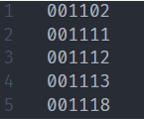
\includegraphics[]{images/all-exam1.png}
    \end{center}
    \caption[ตัวอย่างไฟล์รายวิชาที่มีสอบ]{ตัวอย่างไฟล์รายวิชาที่มีสอบ}
    \label{fig:all_courses}     
\end{figure}
\begin{figure}
    \begin{center}
    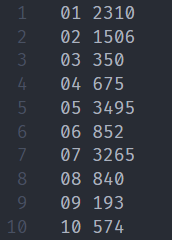
\includegraphics[]{images/capacity1.png}
    \end{center}
    \caption[ตัวอย่างไฟล์ความจุห้องสอบ]{ตัวอย่างไฟล์ความจุห้องสอบ}
    \label{fig:capacity}     
\end{figure}
\begin{figure}
    \begin{center}
      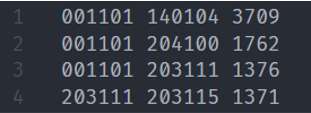
\includegraphics[]{images/conflicts1.png}
    \end{center}
    \caption[ตัวอย่างไฟล์คู่วิชาที่มีนักศึกษาลงทะเบียนพร้อมกัน]{ตัวอย่างไฟล์คู่วิชาที่มีนักศึกษาลงทะเบียนพร้อมกัน}
    \label{fig:conflicts}     
\end{figure}
\begin{figure}
    \begin{center}
      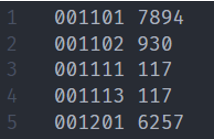
\includegraphics[]{images/courses1.png}
    \end{center}
    \caption[ตัวอย่างไฟล์วิชาที่มีนักศึกษาลงทะเบียน]{ตัวอย่างไฟล์วิชาที่มีนักศึกษาลงทะเบียน}
    \label{fig:courses}     
\end{figure}
\begin{figure}
    \begin{center}
      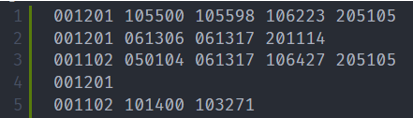
\includegraphics[]{images/regist1.png}
    \end{center}
    \caption[ตัวอย่างไฟล์ลงทะเบียนของนักศึกษา]{ตัวอย่างไฟล์ลงทะเบียนของนักศึกษา}
    \label{fig:regist}     
\end{figure}
\begin{figure}
    \begin{center}
      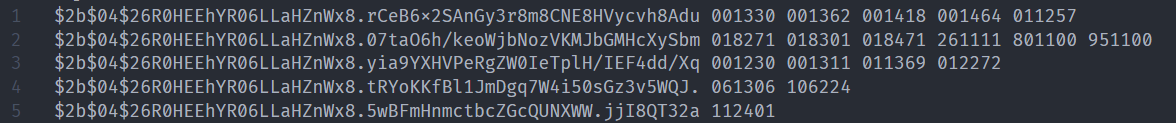
\includegraphics[width=\linewidth]{images/regist_hashed.png}
    \end{center}
    \caption[ตัวอย่างไฟล์ลงทะเบียนของนักศึกษาที่มีรหัสนักศึกษา]{ตัวอย่างไฟล์ลงทะเบียนของนักศึกษาที่มีรหัสนักศึกษา}
    \label{fig:regist_hashed}     
\end{figure}

\begin{itemize}
  \item ในโฟลเดอร์ data ประกอบไปด้วยไฟล์ all-exam-course.in, faculty-capacity.in, conflicts.in,
  enrolled-courses.in, regist.in, regist-studentid.in รวมทั้งหมดจำนวน 6 ไฟล์ แต่ละไฟล์ เป็นไฟล์ text 
  \item ในไฟล์ all-exam-course.in แต่ละบรรทัดประกอบด้วย <รหัสวิชาที่มีการจัดสอบ> หนึ่งบรรทัดต่อหนึ่งรหัสวิชา ตัวอย่างดังภาพที่~\ref{fig:all_courses}
  \item ในไฟล์ faculty-capacity.in แต่ละบรรทัดประกอบด้วย รหัสคณะและจำนวนความจุรวมของห้องสอบของคณะนั้น ๆ มีรูปแบบดังนี้ <รหัสคณะ> <ความจุห้องสอบคณะ> แต่ละส่วนคั่นด้วย เว้นวรรค (space) หนึ่งบรรทัดต่อหนึ่งคณะ ตัวอย่างดังภาพที่~\ref{fig:capacity}
  \item ในไฟล์ conflicts.in แต่ละบรรทัดประกอบด้วย รหัสวิชาสองวิชาที่มีนักศึกษาลงทะเบียนพร้อมกันในภาคการศึกษานั้น ๆ และ จำนวนนักศึกษาที่ลงทะเบียนคู่วิชานี้ มีรูปแบบดังนี้ <รหัสวิชา> <รหัสวิชา> <จำนวนนักศึกษา> แต่ละส่วนคั่นด้วย เว้นวรรค (space) ตัวอย่างดังภาพที่~\ref{fig:conflicts}
  \item ในไฟล์ enrolled-courses.in แต่ละบรรทัดประกอบด้วย รหัสวิชาและจำนวนนักศึกษาที่ลงทะเบียนในวิชานั้น ๆ มีรูปแบบดังนี้ <รหัสวิชา> <จำนวนนักศึกษา> แต่ละส่วนคั่นด้วย เว้นวรรค (space) ตัวอย่างดังภาพที่~\ref{fig:courses}
  \item ในโฟลเดอร์ data/exam-courses-faculty ประกอบไปด้วยไฟล์ 01.in ถึง 21.in ซึ่งเป็นไฟล์ text โดยตั้งชื่อไฟล์ตามรหัสคณะ ในแต่ละไฟล์ประกอบด้วย รหัสวิชาที่มีการจัดสอบ หนึ่งบรรทัดต่อหนึ่งรหัสวิชา ตัวอย่างดังภาพที่~\ref{fig:all_courses} 
  \item ในไฟล์ regist.in แต่ละบรรทัดประกอบด้วย ข้อมูลลงทะเบียนของนักศึกษาหนึ่งคน ประกอบด้วยด้วยรหัสวิชาทั้งหมดที่นักศึกษาคนนั้นลงทะเบียน มีรูปแบบดังนี้ <รหัสวิชา> <รหัสวิชา> <รหัสวิชา> ... แต่ละวิชาคั่นด้วย เว้นวรรค (space) ตัวอย่างดังภาพที่~\ref{fig:regist}
  \item ในไฟล์ regist-studentid.in แต่ละบรรทัดประกอบด้วย ข้อมูลลงทะเบียนของนักศึกษาหนึ่งคน \\ ประกอบด้วยด้วยรหัสนักศึกษาและวิชาทั้งหมดที่นักศึกษาคนนั้นลงทะเบียน มีรูปแบบดังนี้ \\ <รหัสนักศึกษา> <รหัสวิชา> <รหัสวิชา> <รหัสวิชา> ... แต่ละส่วนคั่นด้วย เว้นวรรค (space) \\ ตัวอย่างดังภาพที่~\ref{fig:regist_hashed}
  โดยในตัวอย่างได้มีการ แฮช (hash) รหัสนักศึกษา เพื่อปกป้องข้อมูลส่วนตัวของนักศึกษา
\end{itemize}


\section{วิธีการใช้งานโปรแกรม}
\begin{enumerate}
    \item จัดเตรียมไฟล์ข้อมูลนำเข้าต่าง ๆ ตามที่ได้ระบุไว้ใน \ref{apd:snd_apd} ให้เรียบร้อย
    \item เปิดไฟล์ final\_exam\_graph\_coloring.py
    \item ทำการแก้ไข path ของไฟล์ข้อมูลนำเข้าต่าง ๆ ให้ตรงตามที่กำหนด หากได้ตั้งชื่อไฟล์ และจัดแยกไฟล์ต่าง ๆ ไว้ตามโฟลเดอร์ที่กำหนดแล้วไม่จำเป็นต้องแก้ไขตัวแปร path ใด ๆ
    \item ทำการแก้ไขจำนวน slot ที่ใช้สอบ โดยแก้ไขที่ตัวแปร TOTAL\_SLOTS
\end{enumerate}
ในกรณีที่ต้องการจัดตารางสอบด้วยอัลกอริทึมเพียงวิธีเดียว สามารถเรียกใช้งานโปรแกรมผ่าน console หรือ terminal เช่น cmd หรือ powershell ได้ด้วยคำสั่ง 
\begin{verbatim}
    python final_exam_graph_coloring.py [-OPTION]
\end{verbatim}
ซึ่ง OPTION มีทั้งหมด 4 OPTION ได้แก่ [-deg, -std, -deg-bfs, -std-bfs]

\begin{verbatim}
    ตัวอย่างการเรียกใช้งานโปรแกรม
    python final_exam_graph_coloring.py -deg
\end{verbatim}

\noindent ในกรณีที่ต้องการจัดตารางสอบทั้งหมด 4 วิธี สามารถเรียกใช้งานโปรแกรมผ่าน console หรือ terminal เช่น cmd หรือ powershell ได้ด้วยคำสั่ง
\begin{verbatim}
    python start_scheduler.py
\end{verbatim}
\section{วิธีการใช้งานโปรแกรมคำนวณค่า penalty}
\begin{enumerate}
    \item จัดเตรียมไฟล์ข้อมูลนำเข้าต่าง ๆ ตามที่ได้ระบุไว้ใน \ref{apd:snd_apd} ให้เรียบร้อย
    \item เปิดไฟล์ penalty\_calc.py
    \item ทำการแก้ไข path ของไฟล์ข้อมูลนำเข้าต่าง ๆ ให้ตรงตามที่กำหนด หากได้ตั้งชื่อไฟล์ และจัดแยกไฟล์ต่าง ๆ ไว้ตามโฟลเดอร์ที่กำหนดแล้วไม่จำเป็นต้องแก้ไขตัวแปร path ใด ๆ
    \item ทำการแก้ไขจำนวน slot ที่ใช้สอบให้ตรงกับ solution ของตารางสอบที่จัดโดยโปรแกรม โดยแก้ไขที่ตัวแปร TOTAL\_SLOTS
\end{enumerate}
ในกรณีที่ต้องการคิดคำนวณค่า penalty ของตารางสอบเพียง 1 solution สามารถเรียกใช้งานโปรแกรมผ่าน console หรือ terminal เช่น cmd หรือ powershell ได้ด้วยคำสั่ง 
\begin{verbatim}
    python penalty_calc.py <solution_file>
\end{verbatim}
โดยที่ <solution\_file> คือ path ของไฟล์ solution ตารางสอบที่ได้จากโปรแกรมจัดตารางสอบ

\begin{verbatim}
    ตัวอย่างการเรียกใช้งานโปรแกรมคำนวณค่า penalty
    python penalty_calc.py solution/graph-coloring-solution-deg.txt
\end{verbatim}

\noindent ในกรณีที่ต้องการคิดคำนวณค่า penalty ของตารางสอบทั้งหมด 4 วิธี สามารถเรียกใช้งานโปรแกรมคำนวณค่า penalty ผ่าน console หรือ terminal เช่น cmd หรือ powershell ได้ด้วยคำสั่ง
\begin{verbatim}
    python start_penalty_report.py
\end{verbatim}
โดยให้เปิดไฟล์ start\_penalty\_report.py เพื่อแก้ไขตัวแปร solution\_folder ให้ชี้ไปยังโฟลเดอร์ที่เก็บ solution ตารางสอบทั้งหมดที่เป็น output ของโปรแกรมจัดตารางสอบให้ถูกต้องก่อนการเรียกใช้งานคำสั่งด้านบน

%% Display glossary (optional) -- need glossary option.
\ifglossary\glossarypage\fi

%% Display index (optional) -- need idx option.
\ifindex\indexpage\fi

\begin{biosketch}
\begin{center}
  
\includegraphics[width=1.5in]{mugshot.jpg}
\end{center}
\begin{itemize}[label={},leftmargin=*]
  \item ชื่อ-นามสกุล: นาย ธนวงศ์ เสนีวงศ์ ณ อยุธยา
  \item ระดับการศึกษา: ปริญญาตรี สาขา วิศวกรรมคอมพิวเตอร์ ภาควิชา วิศวกรรมคอมพิวเตอร์
  \item คณะ วิศวกรรมศาสตร์ มหาวิทยาลัยเชียงใหม่
  \item มือถือ: 0899577355 
  \item E-mail: thanawong.saneewong@gmail.com
\end{itemize}


\noindent \textbf{ผลงานและกิจกรรมต่าง ๆ ที่ได้เข้าร่วม}
\begin{itemize}
  \item เข้าร่วมฝึกอบรมค่ายโอลิมปิกวิชาการ สอวน. สาขาคอมพิวเตอร์ ค่าย 1 ปีการศึกษา 2557
  \item เข้าร่วมฝึกอบรมค่ายโอลิมปิกวิชาการ สอวน. สาขาคอมพิวเตอร์ ค่าย 2 ปีการศึกษา 2557
  \item เข้าร่วมฝึกอบรมค่ายโอลิมปิกวิชาการ สอวน. สาขาคอมพิวเตอร์ ค่าย 1 ปีการศึกษา 2558
  \item เป็น staff และผู้ช่วยกรรมการตัดสินในงานแข่งขัน iCode Programming Contest 2018
  \item ผ่านเข้ารอบนำเสนอผลงานและได้รับเงินสนับสนุนการทำโครงงาน ในการแข่งขัน NSC 2021\\
  ที่จัดขึ้นโดย ศูนย์เทคโนโลยีอิเล็กทรอนิกส์และคอมพิวเตอร์แห่งชาติ (NECTEC)
\end{itemize}
\newpage
\begin{center}
  
\includegraphics[width=1.5in]{mugshot.jpg}
\end{center}
\begin{itemize}[label={},leftmargin=*]
  \item ชื่อ-นามสกุล: นาย กฤษฏิ์ อุปนันท์
  \item ระดับการศึกษา: ปริญญาตรี สาขา วิศวกรรมคอมพิวเตอร์ ภาควิชา วิศวกรรมคอมพิวเตอร์
  \item คณะ วิศวกรรมศาสตร์ มหาวิทยาลัยเชียงใหม่
  \item มือถือ: 0954535187
  \item E-mail: krit.upanun@gmail.com
\end{itemize}


\noindent \textbf{ผลงานและกิจกรรมต่าง ๆ ที่ได้เข้าร่วม}
\begin{itemize}
  \item เข้าร่วมแข่งขันการเขียนโปรแกรมคอมพิวเตอร์ระดับมัธยมศึกษา iCode 2014
  \item รางวัลชมเชย การแข่งขันการเขียนโปรแกรมคอมพิวเตอร์ระดับมัธยมศึกษา iCode 2015
  \item เข้าร่วมฝึกอบรมค่ายโอลิมปิกวิชาการ สอวน. สาขาคอมพิวเตอร์ ค่าย 1 ปีการศึกษา 2558
  \item เข้าร่วมฝึกอบรมค่ายโอลิมปิกวิชาการ สอวน. สาขาคอมพิวเตอร์ ค่าย 2 ปีการศึกษา 2558
  \item ผ่านเข้ารอบนำเสนอผลงานและได้รับเงินสนับสนุนการทำโครงงาน ในการแข่งขัน NSC 2021\\
  ที่จัดขึ้นโดย ศูนย์เทคโนโลยีอิเล็กทรอนิกส์และคอมพิวเตอร์แห่งชาติ (NECTEC)
\end{itemize}

\end{biosketch}
\fi % \ifproject
\end{document}
